\documentclass{article}

\usepackage{amsmath,geometry,graphicx,array,makecell,enumitem,bm,booktabs,multirow,pgfplots,bm,amssymb,mathtools,randomwalk,ifthen}
\usepackage[amsmath]{ntheorem}
\usepackage[hidelinks,naturalnames]{hyperref}
\usepackage[nameinlink,noabbrev]{cleveref}
\usepackage{fancyhdr}
\pagestyle{fancy}
\fancyhead[L]{\itshape\nouppercase{\leftmark}}
\fancyhead[R]{B7 Statistical Mechanics}


\title{Statistical Mechanics}
\author{Yue Wu}

\geometry{a4paper,hmargin=1.1in,vmargin=1.2in}

\setlength{\parskip}{1em}
\tolerance=1000
\emergencystretch=1em
\hyphenpenalty=1000
\exhyphenpenalty=100
\righthyphenmin=3

\theoremstyle{plain}\theoremheaderfont{\normalfont\bfseries}\theorembodyfont{\rmfamily}\theoremseparator{.}\newtheorem*{thm}{Theorem}\newtheorem*{law}{Law}\newtheorem*{pos}{Postulate}

\crefname{pos}{Postulate}{Postulates}\crefname{thm}{Theorem}{Theorems}\crefname{law}{Law}{Laws}

\setcounter{tocdepth}{2}
\numberwithin{equation}{section}
\counterwithin{figure}{section}

\newcommand{\qed}{\hfill\ensuremath{\Box}}
\newcommand{\unit}[1]{\ \mathrm{#1}}
\newcommand{\ii}{\mathrm{i}}
\newcommand{\ee}{\mathrm{e}}
\newcommand{\tp}{^\mathrm{T}}
\newcommand{\dbar}{\mathrm{d}\hspace*{-0.14em}\bar{}\hspace*{0.12em}}
\newcommand{\dd}[2][]{\mathrm{d}^{#1} #2\,}
\renewcommand{\d}[2][]{\mathrm{d}^{#1} #2}
\newcommand{\dv}[3][]{\frac{\mathrm{d}^{#1} #2}{{\mathrm{d} #3}^{#1}}}
\newcommand{\pdv}[3][]{\frac{\partial^{#1} #2}{{\partial #3}^{#1}}}
\newcommand{\bra}[1]{\left\langle #1 \right|}
\newcommand{\ket}[1]{\left| #1 \right\rangle}
\newcommand{\braket}[2]{\left\langle #1 \middle| #2 \right\rangle}
\newcommand{\eval}[1]{\left\langle #1 \right\rangle}
\newcommand{\mel}[3]{\left\langle #1 \middle| #2 \middle| #3 \right\rangle}
\newcommand{\expval}[2]{\left\langle #2 \middle| #1 \middle| #2 \right\rangle}
\newcommand{\vb}[1]{\bm{\mathrm{#1}}}
\newcommand{\vdot}{\,\bm{\mathrm{\cdot}}\,}
\newcommand{\abs}[1]{\left| #1 \right|}
\newcommand{\norm}[1]{\left\| #1 \right\|}
\newcommand{\grad}{\vb{\nabla}}
\renewcommand{\div}{\vb{\nabla}\cdot}
\newcommand{\curl}{\vb{\nabla}\times}
\newcommand{\laplacian}{\nabla^2}
\newcommand{\sys}{\text{sys}}
\newcommand{\bath}{\text{bath}}
\newcommand{\tot}{\text{tot}}
\newcommand{\up}{\tikz{\draw[->,very thick,green](0,-0.3)--(0,0.3);}}
\newcommand{\down}{\tikz{\draw[<-,very thick,purple](0,-0.3)--(0,0.3);}}
\DeclareMathOperator{\tr}{tr}
\DeclareMathOperator{\Prob}{Prob}
\newcommand{\fourpoints}{
    \draw[fill = black] (0,0) circle (0.05)node[left]{\small 1};
    \draw[fill = black] (1,0) circle (0.05)node[right]{\small 2};
    \draw[fill = black] (0,1) circle (0.05)node[left]{\small 3};
    \draw[fill = black] (1,1) circle (0.05)node[right]{\small 4};
}
\newcommand{\threepointslb}{
    \draw[fill = black] (0,0) circle (0.05)node[left]{\small 1};
    \draw[fill = black] (1,0) circle (0.05)node[right]{\small 2};
    \draw[fill = black] (0.5,1) circle (0.05)node[left]{\small 3};
}
\newcommand{\threepointsnolb}{
    \draw[fill = black] (0,0) circle (0.07);
    \draw[fill = black] (1,0) circle (0.07);
    \draw[fill = black] (0.5,1) circle (0.07);
}

\newcolumntype{C}[1]{>{\centering\let\newline\\\arraybackslash\hspace{0pt}}m{#1}}

\pgfplotsset{compat=1.18}

\usetikzlibrary{math}

\begin{document}
    \setlength{\parindent}{0pt}
	\Huge\textsf{\textbf{Statistical Mechanics}}
		
	\Large\textsf{\textbf{University of Cambridge Part II Natural Sciences Tripos}}

	\noindent\makebox[\linewidth]{\rule{\textwidth}{2pt}}

	\large\textsf{\textbf{Yue Wu}}
	\begin{itemize}[topsep=0pt,leftmargin=15pt]
		\item[] \textit{Yusuf Hamied Department of Chemistry\\
		Lensfield Road,\\
		Cambridge, CB2 1EW}\\

		\textit{yw628@cam.ac.uk}
	\end{itemize}
    \thispagestyle{empty}
    \pagenumbering{roman}
    \setlength{\parindent}{15pt}

    \newpage
    \begin{center}
		\textbf{\Large{Acknowledgements}}
	\end{center}
	\large
	Nothing in these lecture notes is original. They are largely based on the notes by Dr. Aleks Reinhardt, who lectured this course in 2024. They are nowhere near accurate representations of what was actually lectured, and in particular, all errors are almost surely mine.

    \vskip 30pt

    \begin{center}
		\textbf{\Large{Preface}}
	\end{center}
	\large
    This course assumes a foundational level of understanding in thermodynamics and statistical mechanics --- in particular, the contents that have been lectured in NST Part IA Chemistry \textit{Thermodynamics and Equilibria} and Part IB Chemistry A \textit{Molecular Energy Levels and Thermodynamics}. It may be a little fast for readers without that background. If you are new to thermodynamics/statistical mechanics, but have studied elementary quantum mechanics, an extremely good resource is the course notes on Mathematical Tripos Part II: \textit{Statistical Physics} by Prof. David Tong. You can find it \href{https://www.damtp.cam.ac.uk/user/tong/statphys.html}{\color{blue}here}.

    \normalsize
    \newpage
	\tableofcontents
	\newpage
    \pagenumbering{arabic}

    \section{Introduction}
    \begin{quote}
        \textit{``Anyone who wants to analyze the properties of matter in a real problem might want to start by writing down the fundamental equations and then try to solve them mathematically. Although there are people who try to use such an approach, these people are the failures in this field...''}

        \hfill Richard Feynman
    \end{quote}

    Suppose you know all the fundamental laws of physics, if I give you a box containing \(10^{23}\) particles and tell you their mass, their charge, their interactions, and so on, what can you tell me about the stuff in the box?

    There's one strategy that definitely won't work: writing down the Schr\"{o}dinger equation for \(10^{23}\) particles and solving it. That's typically not trivial to do for 2 or 3 particles, and generally impossible for 23 particles, let alone \(10^{23}\). What's more, even if you could find the wavefunction of the system, what would you do with it? The positions of individual particles are of little interest to anyone. We want answers to much more basic, almost childish, questions about the contents of the box. Is it wet? Is it hot? What colour is it? Is the box in danger of exploding? What happens if we squeeze it, pull it, heat it up? How can we begin to answer these kinds of questions starting from the fundamental laws of physics?

    The purpose of this course is to introduce the dictionary that allows you to translate from the microscopic world where the laws of Nature are written to the everyday macroscopic world that we're familiar with. 

    A large part of this course will be devoted to figuring out the interesting things that happen when you throw \(10^{23}\) particles together. One of the recurring themes will be that
    \begin{equation}
        10^{23}\ne 1\,.
    \end{equation}
    More is different\footnote{Anderson, P. W. (1972). More Is Different: Broken symmetry and the nature of the hierarchical structure of science. Science, 177(4047), 393-396.}: there are key concepts that are not visible in the underlying laws of physics but emerge only when we consider a large collection of particles. One very simple example is temperature. This is not a fundamental concept: it doesn't make sense to talk about the temperature of a single electron. But it would be impossible to talk about physics of the everyday world around us without mentioning temperature. This illustrates the fact that the language needed to describe physics on one scale is very different from that needed on other scales. We'll see several similar emergent quantities in this course, including the phenomenon of phase transitions where the smooth continuous laws of physics conspire to give abrupt, discontinuous changes in the structure of matter.

    Statistical mechanics is the art of turning the microscopic laws of physics into a description of Nature on a macroscopic scale.\footnote{This well-written introduction is from Prof. David Tong.}

    \newpage
    \section{Fundamentals of Statistical Mechanics}
    \subsection{The Microcanonical Ensemble}
    We will start by stating the most fundamental assumption in statistical mechanics. It is the idea that we should take the simplest-minded approach possible and treat all microstates the same --- since we know nothing else about the system, such a democratic approach seems eminently reasonable.
    \begin{pos}[Principle of equal \textit{a priori} probabilities]
        A system with fixed \(N\), \(V\) and \(E\) is equally likely to be found in any of its \(\Omega(E)\) energy eigenstates\footnote{This is not provable. It is the fundamental assumption that the entire Statistical Mechanics is derived upon. Some justifications of this assumption include Boltzmann's H-theorem and Liouville's theorem.}.
    \end{pos}

    Then the probability that the system with fixed energy \(E\) is in a given state \(\ket{n}\) with energy \(E\) is simply
    \begin{equation}
        \Prob(\ket{n})=\frac{1}{\Omega(E)}\,.
    \end{equation}
    The probability that the system is in a state with some different energy \(E'\ne E\) is zero. This type of system with a fixed energy is known as a \textit{microcanonical ensemble}.

    \subsection{Entropy and the Second Law}
    Consider a system with total energy \(E\) that consists of two weakly interacting subsystems, which means that they can only exchange energy, as shown in \cref{Fig:WeaklyCoupledSystems}. The energy is distributed over the two subsystems such that
    \begin{equation}
        E_1+E_2=E\,.
    \end{equation}
    For a given \(E_1\), the total number of degenerate states of the system is \(\Omega_1(E_1)\times\Omega_2(E_2)\). We choose to take the logarithm of the degeneracy so that the value is extensive. This gives
    \begin{equation}
        \ln\Omega(E_1,E-E_1)=\ln\Omega_1(E_1)+\ln\Omega_2(E_2)\,.
    \end{equation}

    \begin{figure}[ht!]
        \centering
        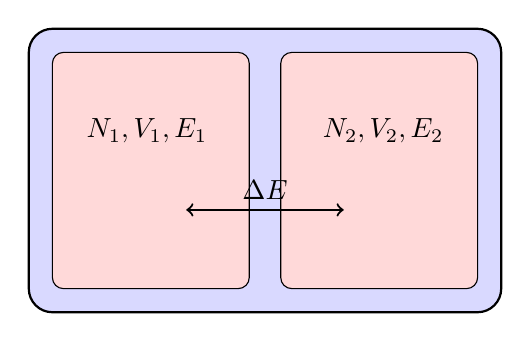
\begin{tikzpicture}
            \draw[thick,rounded corners=0.3 cm,fill=blue!15] (-3,-1.8) rectangle (3,1.8);
            \draw[rounded corners,fill=red!15] (-2.7,-1.5) rectangle (-0.2,1.5);
            \draw[rounded corners,fill=red!15] (2.7,1.5) rectangle (0.2,-1.5);
            \node at (-1.5,0.5) {\(N_1,V_1,E_1\)};
            \node at (1.5,0.5) {\(N_2,V_2,E_2\)};
            \draw[<->,thick] (-1,-0.5)--node[above]{\(\Delta E\)}(1,-0.5);
        \end{tikzpicture}
        \caption{Two weakly coupled systems that can exchange energy such that the total energy of the universe is conserved to be \(E\).}
        \label{Fig:WeaklyCoupledSystems}
    \end{figure}

    By the principle of equal \textit{a priori} probabilities, the most likely value of \(E_1\) is the one that maximises \(\ln\Omega(E_1,E-E_1)\), i.e.
    \begin{equation}
        \left(\pdv{\ln\Omega(E_1,E-E_1)}{E_1}\right)_{N_1,V_1}=0\,.
    \end{equation}
    Using the fact that \(\d{E}_1=-\d{E}_2\), we obtain the condition
    \begin{equation}
        \left(\pdv{\ln\Omega_1(E_1)}{E_1}\right)_{N_1,V_1}=\left(\pdv{\ln\Omega_2(E_2)}{E_2}\right)_{N_2,V_2}\,.
    \end{equation}
    We define
    \begin{equation}
        \beta(E,V,N)\coloneqq\left(\pdv{\ln\Omega(E,V,N)}{E}\right)_{N,V}\,,
    \end{equation}
    then the equilibrium condition becomes
    \begin{equation}
        \beta(E_1,V_1,N_1)=\beta(E_2,V_2,N_2)\,.
    \end{equation}
    Let's examine how this condition is linked to the three laws in thermodynamics.

    \subsubsection{Boltzmann Entropy and the Second Law}
    The thermal equilibrium condition of equal \(\beta\) must be equivalent to the condition that the two subsystems have the same temperature (from classical thermodynamics). Also, just like the thermodynamic entropy \(S\), \(\ln\Omega\) is a state function of \(E\), \(V\) and \(N\). Moreover, when the thermal equilibrium is reached, \(\ln\Omega\) of the total system is maximised, just like the entropy \(S\) should be maximised at equilibrium by the second law of thermodynamics. This suggests that \(\ln\Omega\) is a monotonically increasing function of entropy \(S\). Since both \(S\) and \(\ln\Omega\) are extensive, \(S\) must be proportional to \(\ln\Omega\):
    \begin{equation}
        S(N,V,E)=k_B\ln\Omega(N,V,E)
    \end{equation}
    for some constant \(k_B\) known as \textit{Boltzmann's constant}.

    In the statistical picture, the second law of thermodynamics states that, at thermal equilibrium, the system is most likely to be found in the state that has the largest number of degenerate energy states.

    \subsubsection{Temperature and the First Law}
    The thermodynamic definition of temperature is
    \begin{equation}
        \frac{1}{T}\coloneqq\left(\pdv{S}{E}\right)_{V,N}\,,
    \end{equation}
    which is obtained from the fundamental equation for the internal energy (the first law of thermodynamics)
    \begin{equation}
        \d{E}=T\d{S}-P\d{V}+\mu\d{N}\,.
    \end{equation}
    Hence \(\beta\) and temperature \(T\) is related by
    \begin{equation}
        \beta=\frac{1}{k_B T}\,.
    \end{equation}
    The condition of equal \(\beta\) in statistical mechanics translates to the condition of equal temperature in thermodynamics. 

    \subsubsection{The Third Law}
    The third law of thermodynamics states that at \(T=0\), the entropy of a pure, perfectly crystalline substance is zero, or equally the number of accessible states is equal to one (i.e. \(\Omega=1\), so that \(S=k_B\ln\Omega=0\)). In other words: at absolute zero, the system is in its ground state --- and this ground state is non-degenerate. However, in reality, residual entropy can exist, meaning that as \(T\to 0\), one often observes \(S\) approaching a constant.

    \subsection{The Canonical Ensemble}
    Now let's consider a system that is at thermal equilibrium with a large heat bath. The total system is isolated so that \(E_{\tot}=E_{\bath}+E_{\sys}\) is fixed. The system is weakly coupled to the bath so they can exchange energy. This configuration is commonly called the \textit{canonical ensemble}. Suppose the system is prepared in a specific state \(\ket{i}\) with energy \(E_i\), then the bath has an energy \(E_{\bath}=E_{\tot}-E_i\) with degeneracy \(\Omega_{\bath}(E_{\tot}-E_i)\). The degeneracy of the whole system is \(\Omega=\Omega_{\sys}\Omega_{\bath}=\Omega_{\bath}\). The principle of equal \textit{a priori} probabilities applies only to an isolated system, which is the system plus the bath (the universe) in our case, so all the states of the universe with total energy \(E_{\tot}\) are equally likely to occur. Hence, the probability of finding the system in state \(\ket{i}\) is given by
    \begin{equation}
        \Prob(\ket{i})=\frac{\Omega_{\bath}(E_{\tot}-E_i)}{\sum_{\ket{j}}\Omega_{\bath}(E_{\tot}-E_j)}\,.
    \end{equation}

    \begin{figure}[ht!]
        \centering
        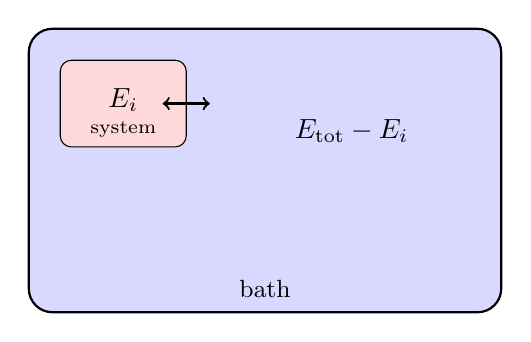
\begin{tikzpicture}
            \draw[thick,rounded corners=0.3 cm, fill=blue!15] (-3,-1.8) rectangle (3,1.8);
            \draw[rounded corners, fill=red!15] (-2.6,0.3) rectangle (-1,1.4);
            \node at (-1.8,0.9) {\(E_i\)};
            \node at (-1.8,0.3)[above]{\scriptsize system};
            \node at (1.1,0.5) {\(E_{\tot}-E_i\)};
            \node at (0,-1.5) {\small bath};
            \draw[<->,thick] (-1.3,0.85)--(-0.7,0.85);
        \end{tikzpicture}
        \caption{The system can exchange energy with the surrounding bath, such that the overall universe has fixed total energy \(E_{\tot}\).}
        \label{Fig:CanonicalEnsemble}
    \end{figure}

    Since the bath is very much larger than the system of interest, most of the energy of the universe will be in the bath. To compute \(\Omega_{\bath}(E_{\tot}-E_i)\), we expand \(\ln\Omega_{\bath}(E_{\tot}-E_i)\) about \(E_{\bath}=E_{\tot}\)
    \begin{equation}\label{canonical_distribution_taylor}
        \ln\Omega_{\bath}(E_{\tot}-E_i)=\ln\Omega_{\bath}(E_{\tot})-E_i\left(\pdv{\ln\Omega_{\bath}(E)}{E}\right)_{E=E_{\tot}}+\mathcal{O}\left(\frac{1}{E_{\bath}}\right)\,,
    \end{equation}
    or,
    \begin{equation}
        \ln\Omega_{\bath}(E_{\tot}-E_i)=\ln\Omega_{\bath}(E_{\tot})-\beta E_i+\mathcal{O}\left(\frac{1}{E_{\bath}}\right)\,.
    \end{equation}
    Hence,
    \begin{equation}\label{canonical_distribution}
        \Prob(\ket{i})=\frac{\exp(-\beta E_i)}{\sum_{\ket{j}}\exp(-\beta E_j)}=\frac{\exp(-\beta E_i)}{Q}\,.
    \end{equation}
    This is the \textit{canonical distribution}, or \textit{Boltzmann Distribution}. It describes the probability of the whole system being found in a particular microstate. The Boltzmann distribution should not be confused with the Maxwell--Boltzmann distribution (the distribution of the particle speeds in ideal gases) or Maxwell--Boltzmann statistics (the distribution of classical particles over energy states in thermal equilibrium).

    In \cref{canonical_distribution_taylor}, we have ignored higher order terms in the Taylor expansion and claimed that it is \(\mathcal{O}(1/E_{\bath})\). This is straightforward to prove. The next term in the expansion is
    \begin{equation}
        \frac{E_i^2}{2}\left(\pdv[2]{\ln\Omega_{\bath}(E)}{E}\right)_{E=E_{\tot}}=\frac{E_i^2}{2}\left(\pdv{\beta}{E}\right)_{E=E_{\tot}}=-\frac{E_i^2}{2k_BT^2C_{V,\bath}}\,,
    \end{equation}
    where we have used
    \begin{equation}
        C_V=\left(\pdv{E}{T}\right)_{N,V}=\left(\pdv{E}{\beta}\right)_{N,V}\left(\pdv{\beta}{T}\right)_{N,V}\,.
    \end{equation}
    Since both heat capacity and total energy are extensive, we can conclude that this term is \(\mathcal{O}(1/E_{\bath})\) as claimed.
    \subsubsection{Link to Thermodynamics}
    Knowing the energy distribution (\ref{canonical_distribution}) allows us to compute the average energy of the system at a given temperature
    \begin{equation}
        \eval{E_{\sys}}=\sum_{\ket{i}}\Prob(\ket{i})E_i=\frac{\sum_{\ket{i}}E_i\exp(-\beta E_i)}{Q}\,.
    \end{equation}
    Next we note that the numerator looks very similar to the definition of \(Q\). If we differentiate \(Q\) with respect to \(\beta\), we obtain the negative of the numerator, and so we can write
    \begin{equation}
        \eval{E_{\sys}}=-\frac{1}{Q}\left(\pdv{Q}{\beta}\right)_{N,V}=-\left(\pdv{\ln{Q}}{\beta}\right)_{N,V}\,.
    \end{equation}
    We can change the differential variable to \(T\) instead
    \begin{equation}
        \eval{E_{\sys}}=-\left(\pdv{\ln Q}{T}\right)_{N,V}\pdv{T}{\beta}=k_B T^2\left(\pdv{\ln Q}{T}\right)_{N,V}\,.
    \end{equation}
    We can compare this to the thermodynamic relation
    \begin{equation}
        E=-T^2\left(\pdv{(A/T)}{T}\right)_{N,V}\,,
    \end{equation}
    which can be easily derived by differentiating \(A/T\), we can see that the Helmholtz free energy \(A\) is related to the partition function through the bridge relation
    \begin{equation}
        A=-k_BT\ln Q\,.
    \end{equation}

    \subsubsection{Fluctuations}
    Back to our canonical ensemble --- a system of \(N\) particles with volume \(V\) in the large thermal bath. The probability of finding the system in any one of the \(\Omega(N,V,E)\) states with energy \(E\) is
    \begin{equation}
        \Prob(E)=\frac{\Omega(N,V,E)\exp(-\beta E)}{\sum_{\ket{i}}\exp(-\beta E_i)}\,.
    \end{equation}
    Using the definition of entropy, we may rewrite this as
    \begin{equation}\label{canonical_energy_probability}
        \Prob(E)\sim\exp(-\beta E)\exp\left[\frac{S(N,V,E)}{k_B}\right]\,.
    \end{equation}
    The most likely energy of the system, \(E^*\), is the one for which
    \begin{equation}
        \left.\pdv{\Prob(E)}{E}\right|_{E=E^*}=0\quad\Rightarrow\quad\left(\pdv{S}{E}\right)_{E=E^*}=\frac{1}{T}\,.
    \end{equation}
    We can expand \(S\) in a Taylor series about \(E^*\) and define \(\Delta E\coloneqq E-E^*\), we obtain
    \begin{equation}\label{canonical_entropy_expansion}
        \frac{S(N,V,E)}{k_B}=\frac{S(N,V,E^*)}{k_B}+\frac{1}{k_BT}\Delta E+\frac{1}{2k_B}\left(\pdv[2]{S}{E}\right)(\Delta E)^2+\mathcal{O}((\Delta E)^3)\,.
    \end{equation}
    Take the logarithm of expression (\ref{canonical_energy_probability}) and use the expansion (\ref{canonical_entropy_expansion}), we can see that
    \begin{equation}
        \ln \Prob(E^*+\Delta E)=c+\frac{1}{2k_B}\left(\pdv[2]{S}{E}\right)(\Delta E)^2+\mathcal{O}((\Delta E)^3)\,,
    \end{equation}
    where \(c\) is some constant independent of \(\Delta E\). The term linear in \(\Delta E\) vanishes. In the limit of large \(N\), we can ignore terms of order \((\Delta E)^3\) or above and find that
    \begin{equation}
        \Prob(E^*+\Delta E)=c'\exp\left[\frac{1}{2k_B}\left(\pdv[2]{S}{E}\right)(\Delta E)^2\right]\,,
    \end{equation}
    where \(c'\) is another constant. We now recall the standard thermodynamics relation
    \begin{equation}
        \left(\pdv[2]{S}{E}\right)=\left(\pdv{(1/T)}{E}\right)_V=-\frac{1}{T^2}\left(\pdv{T}{E}\right)_V=-\frac{1}{T^2}\left(\pdv{E}{T}\right)_{V}^{-1}=-\frac{1}{C_V T^2}\,.
    \end{equation}
    Finally, we normalise the probability density to obtain
    \begin{equation}
        \Prob(E^*+\Delta E)=(2\pi k_B T^2 C_V)^{-1/2}\exp\left[-\frac{(\Delta E)^2}{2k_B T^2C_V}\right]\,,
    \end{equation}
    or
    \begin{equation}
        \Prob(E)=(2\pi k_B T^2 C_V)^{-1/2}\exp\left[-\frac{(E-E^*)^2}{2k_B T^2C_V}\right]\,.
    \end{equation}
    This is a Gaussian distribution. We find that the mean squared fluctuation in the energy of a system at constant \(N\), \(V\) and \(T\) is directly related to the heat capacity \(C_V\),
    \begin{equation}
        \sigma_E^2=\eval{(\Delta E)^2}=k_BT^2C_V\,.
    \end{equation}

    In fact, whilst the result that the probability distribution function is a Gaussian is important, it is possible to compute the variance of the distribution in a much simpler way if we are only interested in it. The thermal average of the energy is
    \begin{equation}
        \eval{E}=\frac{\sum_{\ket{i}}E_i \ee^{-\beta E_i}}{Q}=-\frac{1}{Q}\pdv{Q}{\beta}\,,
    \end{equation}
    and hence the derivative of \(\eval{E}\) with respect to \(\beta\) is
    \begin{equation}
        \pdv{\eval{E}}{\beta}=-\frac{\sum_{\ket{i}}E_i^2 \ee^{-\beta E_i}}{Q}+\left(\frac{1}{Q}\pdv{Q}{\beta}\right)^2\,.
    \end{equation}
    This can be simplified to
    \begin{equation}
        \pdv{\eval{E}}{\beta}=-\eval{E^2}+\eval{E}^2\equiv -\sigma_E^2\,.
    \end{equation}
    We can relate this to the heat capacity at constant volume
    \begin{equation}
        C_V=\left(\pdv{E}{T}\right)_{N,V}=\left(\pdv{E}{\beta}\right)_{N,V}\pdv{\beta}{T}=-\frac{1}{k_BT^2}\left(\pdv{E}{\beta}\right)_{N,V}\,.
    \end{equation}
    Therefore \(\sigma_E^2=k_BT^2 C_V\) as before.

    Since both \(E\) and \(C_V\) are extensive, we can write \(\eval{E}=N\eval{\epsilon}\) and \(C_V=Nc_V\), where \(\epsilon\) and \(c_V\) are the energy and heat capacity per particle. The relative variance in the energy vanishes in the thermodynamic limit as \(N\to\infty\), since
    \begin{equation}
        \frac{\eval{(\Delta E)^2}}{\eval{E}^2}=k_BT^2\frac{C_V}{\eval{E}^2}=\frac{k_BT^2c_V}{N\eval{\epsilon}^2}\sim\frac{1}{N}\,.
    \end{equation}
    Similar results apply to other quantities of interest. Fluctuations about the average are negligible in the thermodynamic limit, and the statistical mechanical average of a thermodynamic property will correspond to its measured value.

    \subsubsection{Helmholtz Energy and Equilibrium}
    By the second law of thermodynamics, in an isolated system at equilibrium, the entropy of a system is maximised. In the canonical ensemble, a system is in contact with a thermal reservoir. Although heat can be transferred between them, the total energy is conserved. The system plus the thermal bath is isolated, so we may apply the second law of thermodynamics. The total degeneracy is
    \begin{equation}
        \Omega_{\tot}=\Omega_{\sys}(E_{\sys})\Omega_{\bath}(E_{\tot}-E_{\sys})\,.
    \end{equation}
    We can Taylor expand \(\ln{\Omega_{\bath}(E_{\tot}-E_{\sys})}\) up to linear order in \(E_{\sys}\) and find that
    \begin{equation}
        \ln{\Omega_{\tot}}=\ln{\Omega_{\sys}(E_{\sys})}+\ln{\Omega_{\bath}(E_{\tot})}-\beta E_{\sys}\,.
    \end{equation}
    The equilibrium condition is that the derivative of \(\ln{\Omega_{\tot}}\) with respect to \(E_{\sys}\) vanishes. Since \(\ln\Omega_{\bath}(E_{\tot})\) is independent of \(E_{\sys}\), the equilibrium condition is equivalent to minimising \(\beta E_{\sys}-\ln{\Omega_{\sys}(E_{\sys})}=\beta(E_{\sys}-TS_{\sys})\). The Helmholtz energy \(A\) is defined as
    \begin{equation}
        A\coloneqq E-TS\,.
    \end{equation}
    Therefore, at constant temperature and volume, \(A\) is at a minimum at equilibrium.

    \subsection{Pressure}
    Now consider a system that can exchange volume with a reservoir such that the total volume of the system plus the bath is fixed. The condition for equilibrium is that the total entropy is maximised, so we need to determine the maximum of
    \begin{equation}
        \ln{\Omega(V_{\sys},V_{\tot}-V_{\sys})}=\ln{\Omega_{\sys}(V_{\sys})}+\ln\Omega_{\bath}(V_{\tot}-V_{\sys})
    \end{equation}
    with respect to \(V_{\sys}\). Using the definition of entropy,
    \begin{equation}
        \left(\pdv{S_{\sys}}{V_{\sys}}\right)_{E,N}+\left(\pdv{S_{\bath}}{V_{\sys}}\right)_{E,N}=0\,.
    \end{equation}
    Since \(\d{V_{\sys}}=-\d{V_{\bath}}\),
    \begin{equation}
        \left(\pdv{S_{\sys}}{V_{\sys}}\right)_{E,N}=\left(\pdv{S_{\bath}}{V_{\bath}}\right)_{E,N}\,.
    \end{equation}
    From thermodynamics, we have
    \begin{equation}
        \d{S}=\frac{1}{T}\d{E}+\frac{P}{T}\d{V}-\frac{\mu}{T}\d{N}
    \end{equation}
    and hence \((\partial S/\partial V)_{E,N}=P/T\). Thus the equilibrium condition becomes
    \begin{equation}
        \frac{P_{\sys}}{T_{\sys}}=\frac{P_{\bath}}{T_{\bath}}\,.
    \end{equation}
    If the system can exchange both energy and volume with the bath, then the conditions for equilibrium are \(T_{\sys}=T_{\bath}\) and \(P_{\sys}=P_{\bath}\).

    \begin{figure}
        \centering
        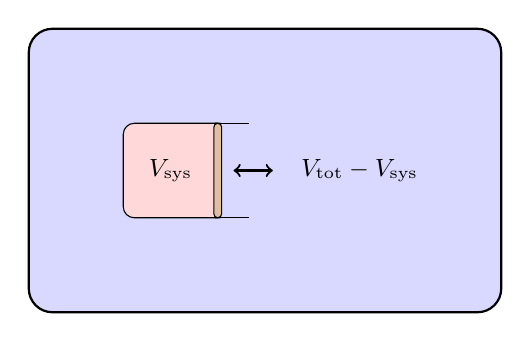
\begin{tikzpicture}
            \draw[thick,rounded corners=0.3 cm, fill=blue!15] (-3,-1.8) rectangle (3,1.8);
            \draw[rounded corners, fill=red!15] (-0.6,0.6)--(-1.8,0.6)--(-1.8,-0.6)--(-0.6,-0.6);
            \draw[rounded corners=0.05 cm, fill=brown!50] (-0.65,-0.6) rectangle (-0.55,0.6); 
            \draw (-0.6,0.6)--(-0.2,0.6);
            \draw (-0.6,-0.6)--(-0.2,-0.6);
            \draw[<->,thick] (-0.4,0)--(0.1,0);
            \node at (-1.2,0) {\small \(V_{\sys}\)};
            \node at (1.2,0) {\small \(V_{\tot}-V_{\sys}\)};
        \end{tikzpicture}
        \caption{A system coupled to the bath such that a piston separating them can change position. The system and the bath can exchange volume.}
    \end{figure}

    In practice, it is convenient to use the fundamental relation for the Helmholtz energy, \(\d{A}=-S\d{T}-P\d{V}+\mu\d{N}\), and the corresponding expression for the pressure
    \begin{equation}
        P=-\left(\pdv{A}{V}\right)_{T,N}=k_BT\left(\pdv{\ln Q}{V}\right)_{T,N}\,,
    \end{equation}
    where we have used the bridge relation \(A=-k_B T\ln Q\). Later, we shall use the relation to obtain a general expression of the pressure in a system of interacting particles. However, we will need to first derive some further results in classical statistical mechanics.
    \subsection{Classical Statistical Mechanics}
    The thermal average of the expectation value of some observable \(X\) is
    \begin{equation}
        \eval{X}=\sum_{\ket{i}}\Prob(\ket{i})\expval{X}{i}=\frac{\sum_{\ket{i}}\exp(-\beta E_i)\expval{X}{i}}{\sum_{\ket{i}}\exp(-\beta E_i)}\,.
    \end{equation}
    This suggests that in order to compute the thermal average, we first need to solve the Schr\"{o}dinger equation of the many-body system of interest to obtain the eigenstates \(\ket{i}\), then we need to compute the expectation value of the operator \(X\) for all those quantum states that have non-negligible statistical weight. This approach is doomed for all but the simplest systems. Fortunately, this can be simplified to a more workable expression in the classical limit \(h\to 0\). For a \(d\)-dimensional, \(N\)-particle system, this is given by\footnote{The derivation is in the appendix \cref{Chap:Quantum_to_Classical}}
    \begin{equation}
        \eval{X}=\frac{\int\prod_{i=1}^{N}\dd[d]{\vb{p}_i}\dd[d]{\vb{r}_i}\exp\left[-\beta H(\{\vb{p}_i\},\{\vb{r}_i\})\right]X(\{\vb{p}_i\},\{\vb{r}_i\})}{\int\prod_{i=1}^{N}\dd[d]{\vb{p}_i}\dd[d]{\vb{r}_i}\exp\left[-\beta H(\{\vb{p}_i\},\{\vb{r}_i\})\right]}\,,
    \end{equation}
    where \(\vb{r}_i\) and \(\vb{p}_i\) are the coordinate and momentum of the \(i^{\text{th}}\) particle and 
    \begin{equation}
        H(\{\vb{p}_i\},\{\vb{r}_i\})=\sum_{i}^{N}\frac{p_i^2}{2m_i} + U(\{\vb{r}_i\})
    \end{equation}
    is the classical Hamiltonian. The classical partition function is
    \begin{equation}
        Q=\frac{1}{h^{dN}N!}\int\prod_{i=1}^{N}\dd[d]{\vb{p}_i}\dd[d]{\vb{r}_i}\exp\left[-\beta H(\{\vb{p}_i\},\{\vb{r}_i\})\right]\,,
    \end{equation}
    where the \(1/N!\) factor is to account for the indistinguishability of the particles\footnote{The situation is actually a bit subtle\dots\ See \textit{Gibbs' Paradox}.} and \(1/h^{dN}\) is to make the partition function dimensionless.
    \subsubsection{Integration over the Momenta}
    From now on, we assume that the space is three-dimensional and all particles have the same mass \(m\), although both conditions can be easily generalised. Note that due to the form of the Hamiltonian, the integration over momenta and spatial coordinates can be separated
    \begin{equation}
        Q(N,V,T)=\frac{1}{h^{3N}N!}\int\prod_{i=1}^{N}\dd[3]{\vb{p}_i}\exp\left(-\beta\sum_{i=1}^{N}\frac{p_i^2}{2m}\right)\int\prod_{i=1}^{N}\dd[3]{\vb{r}_i}\exp(-\beta U(\{\vb{r}_i\}))\,.
    \end{equation}
    Let's focus on the first integral. We can resolve \(\vb{p}_i\) into its Cartesian components \(p_i^2=p_{ix}^2+p_{iy}^2+p_{iz}^2\), so it can be further factorised as
    \begin{align}
        &\int\prod_{i=1}^{N}\dd[3]{\vb{p}_i}\exp\left(-\beta\sum_{i=1}^{N}\frac{p_i^2}{2m}\right)\notag\\
        &\qquad\qquad\qquad= \int\prod_{i=1}^{N}\dd{p_{ix}}\dd{p_{iy}}\dd{p_{iz}}\exp\left(-\frac{\beta p_{ix}^2}{2m}\right)\exp\left(-\frac{\beta p_{iy}^2}{2m}\right)\exp\left(-\frac{\beta p_{iz}^2}{2m}\right)\,.
    \end{align}
    These are just \(3N\) identical Gaussian integrals, each evaluated as
    \begin{equation}
        \int_{-\infty}^{\infty}\dd{p}\exp\left(-\frac{\beta p^2}{2m}\right)=\sqrt{\frac{2m\pi}{\beta}}\,.
    \end{equation}
    Hence, the partition function can be written as
    \begin{align}
        Q(N,V,T)&=\frac{1}{h^{3N}N!}\left(\frac{2m\pi}{\beta}\right)^{3N/2}\int\prod_{i=1}^{N}\dd[3]{\vb{r}_i}\exp[-\beta U(\{\vb{r}_i\})] \notag\\
        &\eqqcolon\frac{1}{\Lambda^{3N}N!}\int\prod_{i=1}^N\dd[3]{\vb{r}_i}\exp[-\beta U(\{\vb{r}_i\})]\,,
    \end{align}
    where \(\Lambda\coloneqq h/\sqrt{2\pi mk_BT}\) is the \textit{de Broglie wavelength}. If the system consists of a mixture of two components \(A\) and \(B\), then the classical partition function becomes
    \begin{equation}
        Q(N_A,N_B,V,T)=\frac{1}{\Lambda_A^{3N_A}\Lambda_B^{3N_B}N_A!N_B!}\int\prod_{i=1}^{N_A}\prod_{j=1}^{N_B}\dd[3]{\vb{r}_i}\dd[3]{\vb{r}_j}\exp[-\beta U(\{\vb{r}_i\},\{\vb{r}_j\})]\,.
    \end{equation}
    In molecular systems, a purely classical description is inappropriate. In particular, the internal energy levels of molecules like electronic energies, vibrations and rotations are not accounted for by the classical Hamiltonian. Then the classical partition function must have the form
    \begin{equation}
        Q(N,V,T)=\frac{q_{\text{intra}}^N}{\Lambda^{3N}N!}\int\prod_{i=1}^{N}\dd[3]{\vb{r}_i}\exp[-\beta U(\{\vb{r}_i\})]\,,
    \end{equation}
    where \(q_{\text{intra}}\) is the partition sum over all molecular energy levels
    \begin{equation}
        q_{\text{intra}}=\sum_{i}\exp(-\beta\epsilon_i)\,.
    \end{equation}
    It often has the form
    \begin{equation}
        q_{\text{intra}}=q_{\text{vib}}q_{\text{rot}}q_{\text{elec}}\,.
    \end{equation}
    \subsubsection{Classical Ideal Gas}
    Consider a classical ideal gas, where there is no interaction between particles. The Hamiltonian of the system is given only by the kinetic energy contribution
    \begin{equation}
        H_{\text{ideal}}(\{\vb{r}_i\},\{\vb{p}_i\})=\sum_{i=1}^{N}\frac{p_i^2}{2m}\,.
    \end{equation}
    Since there is no interaction between particles, \(U=0\), the partition function is given by
    \begin{equation}
        Q_{\text{ideal}}(N,V,T)=\frac{1}{\Lambda^{3N}N!}\int\prod_{i=1}^{N}\dd[3]{\vb{r}_i}=\frac{V^N}{\Lambda^{3N}N!}\,.
    \end{equation}
    Hence,
    \begin{equation}
        A=-k_B T\ln Q_{\text{ideal}}=-k_B T\ln\left(\frac{V^N}{\Lambda^{3N}N!}\right)\,,
    \end{equation}
    and from the fundamental equation \(\d{A}=-S\d{T}-P\d{V}+\mu\d{N}\), the expression for the pressure is
    \begin{equation}
        P_{\text{ideal}}=-\left(\pdv{A}{V}\right)_{N,T}=\frac{Nk_B T}{V}\,.
    \end{equation}
    This is the well-known \textit{ideal gas equation}, which can be rewritten in a perhaps more familiar form
    \begin{equation}
        PV=nRT\,.
    \end{equation}
    \subsection{Other Ensembles}
    There are five common ensembles that we usually consider
    \begin{enumerate}[topsep=0pt,label=(\roman*)]
        \item \textit{Microcanonical (\(NVE\)) ensemble}: an isolated system;
        \item \textit{Canonical (\(NVT\)) ensemble}: can exchange energy with the bath;
        \item \textit{Isothermal-isobaric (\(NPT\)) ensemble}: can exchange both energy and volume with the bath;
        \item \textit{Isoenthalpic-isobaric (\(NPH\)) ensemble}: can exchange volume with the bath;
        \item \textit{Grand canonical (\(\mu VT\)) ensemble}: can exchange particles and energy with the bath.
    \end{enumerate}

    We have already encountered microcanonical ensemble and canonical ensemble. Now let's consider an isothermal-isobaric ensemble: a system with \(N\) particles that can exchange energy and volume with a large reservoir. The probability of finding the system at a given microstate \(\ket{i}\) with energy \(E_i\) and volume \(V_i\) is determined by \(\Omega_{\bath}(E_{\tot}-E_i,V_{\tot}-V_i)\). By Taylor expansion as before, and using
    \begin{equation}
        \left(\pdv{S}{E}\right)_{N,V}=\frac{1}{T}\,,\;\left(\pdv{S}{V}\right)_{E,N}=\frac{P}{T}\,,
    \end{equation}
    we get
    \begin{equation}
        \ln{\Omega_{\bath}(E_{\tot}-E_i,V_{\tot}-V_i)}=\ln{\Omega_{\bath}(E_{\tot},V_{\tot})}-\frac{E_i+PV_i}{k_BT}\,,
    \end{equation}
    where \(E_i+PV_i\eqqcolon H_i\) is the \textit{enthalpy}. The probability of finding the system with volume \(V_i\) is therefore given by
    \begin{equation}
        \Prob(V_i)=\frac{Q(N,V_i,T)\ee^{-\beta PV_i}}{\Delta}\,,
    \end{equation}
    where \(\Delta\) is the \textit{isothermal-isobaric partition function} quantum mechanically defined as
    \begin{equation}
        \Delta\coloneqq\sum_{V_i}Q(N,V_i,T)\ee^{-\beta PV_i}\,.
    \end{equation}
    Classically, it is defined as
    \begin{equation}
        \Delta\coloneqq\beta P\int_{0}^{\infty}\dd{V}Q(N,V,T)\ee^{-\beta PV}\,,
    \end{equation}
    where \(\beta P\) is to make the quantity dimensionless, and correspondingly the probability density of finding the system with volume \(V_i\) is
    \begin{equation}
        p(V_i)=\frac{\beta P Q(N,V_i,T)\ee^{-\beta PV_i}}{\Delta}\,.
    \end{equation}
    As for other ensembles, we have the bridge relationship
    \begin{equation}
        G=-k_BT\ln\Delta\,.
    \end{equation}

    Another ensemble of great importance is the grand canonical ensemble. Consider a system of volume \(V\) that can exchange particles and energy with the reservoir. The probability of finding the system in a state with \(N_i\) particles and energy \(E_i\) is determined by \(\Omega_{\bath}(E_{\tot}-E_i,N_{\tot}-N_i)\). Using
    \begin{equation}
        \left(\pdv{S}{N}\right)_{E,V}=-\frac{\mu}{T}\,,
    \end{equation}
    we get
    \begin{equation}
        \Prob(N_i)=\frac{Q(N_i,V,T)\exp(\beta\mu N_i)}{\Xi}\,,
    \end{equation}
    where
    \begin{equation}
        \Xi\coloneqq\sum_{N=0}^{\infty}Q(N,V,T)\exp(\beta\mu N)=\sum_{N=0}^{\infty}Q(N,V,T)z^N,
    \end{equation}
    is the \textit{grand partition function} and \(z\coloneqq \ee^{\beta\mu}\) is the \textit{absolute activity} (or sometimes loosely called \textit{fugacity}). The \textit{grand potential} (\textit{Landau potential}), defined as\footnote{The second equality below follows from the fact that \(\Phi\) is extensive, while among the natural variables \(T,V,N\), only \(V\) is extensive, so \(\Phi\) must be proportional to \(V\). If you don't trust this relation, you can check appendix \ref{Chap:Thermodynamics} for a formal proof.}
    \begin{equation}
        \Phi=E-TS-N\mu=-PV\,,
    \end{equation}
    is related to the grand partition function by the bridge relation
    \begin{equation}
        \Phi=-k_B T\ln\Xi\,.
    \end{equation}
    The average number of particles in the system is
    \begin{equation}
        \eval{N}=\left(\pdv{\ln\Xi}{\beta\mu}\right)_{V,T}\,.
    \end{equation}

    \begin{table}[ht!]
        \centering
        \begin{tabular}{cc}
            \begin{tabular}{C{6.5cm}}
                \toprule
                \textit{microcanonical ensemble} \\
                constant \(N,V,E\)\\ \midrule
                \vskip -1 cm
                \[ S=k_B\ln\Omega(N,V,E) \] 
                \[ \d{E}=T\d{S}-P\d{V}+\mu\d{N} \]
                \[ (1/T)=(\partial S/\partial E)_{N,V} \]
                \[ P=T(\partial S/\partial V)_{E,N} \]
                \[ \mu=-T(\partial S/\partial N)_{E,V} \]
                \vskip -1 cm \\ \bottomrule
            \end{tabular} & \begin{tabular}{C{6.5cm}}
                \toprule
                \textit{canonical ensemble} \\
                constant \(N,V,T\)\\ \midrule
                \vskip -1 cm
                \[ A=E-TS=-k_BT\ln Q(N,V,T) \] 
                \[ \d{A}=-S\d{T}-P\d{V}+\mu\d{N} \]
                \[ E=(\partial (\beta A)/\partial \beta)_{N,V} \]
                \[ P=-(\partial A/\partial V)_{N,T} \]
                \[ \mu=(\partial A/\partial N)_{V,T} \]
                \vskip -1 cm \\ \bottomrule
            \end{tabular} \\
             & \\
            \begin{tabular}{C{6.5cm}}
                \toprule
                \textit{isothermal-isobaric ensemble} \\
                constant \(N,P,T\)\\ \midrule
                \vskip -1 cm
                \[ G=A+PV=N\mu=-k_BT\ln\Delta(N,P,T) \] 
                \[ \d{G}=-S\d{T}+V\d{P}+\mu\d{N} \]
                \[ H=E+PV=(\partial (\beta G)/\partial \beta)_{N,P} \]
                \[ V=(\partial G/\partial P)_{N,T} \]
                \[ \mu=(\partial G/\partial N)_{P,T} \]
                \vskip -1 cm \\ \bottomrule
            \end{tabular} & \begin{tabular}{C{6.5cm}}
                \toprule
                \textit{grand canonical ensemble} \\
                constant \(\mu,V,T\)\\ \midrule
                \vskip -1 cm
                \[ \Phi=A-\mu N=-PV=-k_BT\ln \Xi(\mu,V,T) \] 
                \[ \d{\Phi}=-S\d{T}-P\d{V}-N\d{\mu} \]
                \[ N=-(\partial \Phi/\partial \mu)_{V,T} \]
                \[ P=-(\partial \Phi/\partial V)_{T,\mu} \]
                \[ E=N\mu+(\partial (\beta\Phi)/\partial \beta)_{\mu,V} \]
                \vskip -1 cm \\ \bottomrule
            \end{tabular}
        \end{tabular}\caption{Common ensembles and related relations.}
    \end{table}

    It is possible to generate a lot more different ensembles by different combinations of Legendre transforms; however, the microcanonical, canonical and grand canonical ensembles are the most important ones (as you can tell from their names).

    \subsubsection{Langmuir Adsorption}
    Why do we need different ensembles? In fact you will show in one of the exercises that in the thermodynamic limit, all the ensembles are equivalent. However, some calculations may be more difficult in one ensemble than another. The choice of ensemble is primarily a matter of convenience.

    As an illustration, consider the adsorption of gas molecules on the metal surface. Assume the metal has \(M\) sites, each can accommodate one molecule at most, and if a particle is adsorbed, its energy is lowered by \(\epsilon\). The gas has chemical potential \(\mu\).

    First, let's solve this question in the canonical ensemble. If \(N\) particles are adsorbed, the energy of the system is
    \begin{equation}
        E(N)=-N\epsilon\,,
    \end{equation}
    and the degeneracy of this energy of the system is
    \begin{equation}
        \Omega(N)=\frac{M!}{N!(M-N)!}\,.
    \end{equation}
    The canonical partition function is therefore
    \begin{equation}
        Q(N,M,T)=\frac{M!}{N!(M-N)!}\exp(\beta N\epsilon)\,.
    \end{equation}
    The chemical potential is
    \begin{equation}
        \mu=-k_B T\left(\pdv{\ln Q}{N}\right)_{V,T}=-\epsilon+k_B T(\ln N-\ln(M-N))
    \end{equation}
    by Stirling's approximation. Define the density of adsorbed particles as \(\rho\coloneqq N/M\), then
    \begin{equation}
        \mu +\epsilon=k_B T\ln\left(\frac{\rho}{1-\rho}\right)\,.
    \end{equation}
    By rearranging, we get
    \begin{equation}
        \rho=\frac{1}{1+\exp[-\beta(\mu+\epsilon)]}\,.
    \end{equation}

    Now let's derive the same result in the grand canonical ensemble.
    \begin{align}
        \Xi&=\sum_{N=0}^{M}\frac{M!}{N!(M-N)!}\exp[N\beta(\mu+\epsilon)]\notag\\
        &=\left(1+\exp[\beta(\mu+\epsilon)]\right)^M
    \end{align}
    by the binomial theorem. The average number of particles is therefore
    \begin{equation}
        \eval{N}=\left(\pdv{\ln\Xi}{\beta\mu}\right)_{M,T}=\frac{M\exp[\beta(\mu+\epsilon)]}{1+\exp[\beta(\mu+\epsilon)]}\,.
    \end{equation}
    It immediately follows that
    \begin{equation}
        \eval{\rho}=\frac{1}{1+\exp[-\beta(\mu+\epsilon)]}
    \end{equation}
    as calculated before.
    \subsection{Pressure of Interacting Particles}
    \subsubsection{Pressure from the Partition Function}
    Consider a system of interacting gas particles in a cubic box with edge length \(L=V^{1/3}\). Define the scaled coordinate
    \begin{equation}
        \vb{s}_i=\frac{\vb{r}_i}{L}\,,
    \end{equation}
    so that each component of \(\vb{s}_i\) ranges between zero and unity. We can then write
    \begin{equation}
        Q(N,V,T)=\frac{V^N}{\Lambda^{3N}N!}\int_{0}^{1}\dots\int_{0}^{1}\prod_{i=1}^{N}\dd[3]{\vb{s}_i}\exp[-\beta U(\{\vb{s}_i\};L)],
    \end{equation}
    where we have included \(L\) as the parameter of \(U\) to indicate that \(U\) depends on the real rather than the scaled distances between the particles. The pressure is therefore
    \begin{align}
        P&=k_BT\left(\pdv{\ln V^N}{V}\right)_{T,N}+k_B T\left(\pdv{}{V}\ln\int_{0}^{1}\dots\int_{0}^{1}\prod_{i=1}^{N}\dd[3]{\vb{s}_i}\exp[-\beta U(\{\vb{s}_i\};L)]\right)_{T,N}\notag\\
        &=\frac{Nk_B T}{V}-\frac{1}{\int\prod_{i=1}^{N}\dd[3]{\vb{s}_i}\exp[-\beta U(\{\vb{s}_i\};L)]}\int\prod_{i=1}^{N}\dd[3]{\vb{s}_i}\exp[-\beta U(\{\vb{s}_i\};L)]\pdv{U(\{\vb{s}_i\};L)}{V}\notag\\
        &=\underbrace{\frac{Nk_B T}{V}}_{\text{ideal}}-\underbrace{\eval{\pdv{U(\{\vb{s}_i\};L)}{V}}}_{\text{non-ideal}}\,.
    \end{align}
    We clearly see an ideal contribution and a non-ideal contribution which arise only if the particles are interacting (\(U\ne 0\)).

    We now use the chain rule
    \begin{equation}
        \pdv{U(\{\vb{s}_i\};L)}{V}=\sum_{i=1}^{N}\sum_{k=1}^{3}\pdv{U(\{\vb{s}_i\};L)}{r_{ik}}\pdv{r_{ik}}{V}\,,
    \end{equation}
    where \(k\in\{1,2,3\}\) labelling the component. We have
    \begin{equation}
        \pdv{r_{ik}}{V}=\pdv{Ls_{ik}}{V}=s_{ik}\pdv{V^{1/3}}{V}=\frac{s_{ik}}{3V^{2/3}}=\frac{r_{ik}}{3V}\,.
    \end{equation}
    Hence
    \begin{equation}
        \pdv{U(\{\vb{s}_i\};L)}{V}=\sum_{i=1}^{N}\sum_{k=1}^{3}\pdv{U(\{\vb{s}_i\};L)}{r_{ik}}\frac{r_{ik}}{3V}\,.
    \end{equation}
    For conservative forces, \(\vb{f}=-\grad U\), so
    \begin{equation}
        \pdv{U(\{\vb{r}_i\})}{r_{ik}}=-f_{ik}\,.
    \end{equation}
    Therefore,
    \begin{equation}
        P=\frac{Nk_BT}{V}+\frac{1}{3V}\eval{\sum_{i=1}^{N}\vb{f}_i\vdot\vb{r}_i}\,.
    \end{equation}
    \subsubsection{Pressure for Pairwise-additive Forces}
    Consider the special case that the intermolecular forces are pairwise-additive such that
    \begin{equation}
        \vb{f}_i=\sum_{j\ne i}\vb{f}_{ij}\,,
    \end{equation}
    where \(\vb{f}_{ij}\) is the force on particle \(i\) exerted by particle \(j\). Then
    \begin{equation}
        P=\frac{Nk_BT}{V}+\eval{\sum_{i=1}^{N}\sum_{j\ne i}^{N}\frac{1}{3V}\vb{r}_i\vdot\vb{f}_{ij}}\,.
    \end{equation}
    If we permute the dummy indices \(i\) and \(j\), we get
    \begin{equation}
        P=\frac{Nk_BT}{V}+\eval{\sum_{j=1}^{N}\sum_{i\ne j}^{N}\frac{1}{3V}\vb{r}_j\vdot\vb{f}_{ji}}\,.
    \end{equation}
    By Newton's third law, we get
    \begin{equation}
        P=\frac{Nk_BT}{V}+\frac{1}{6V}\eval{\sum_{i=1}^{N}\sum_{j\ne i}^{N}\vb{r}_{ij}\vdot\vb{f}_{ij}}\,,
    \end{equation}
    where \(\vb{r}_{ij}\coloneqq\vb{r}_i-\vb{r}_j\). This can be rewritten in the dimensionless form as
    \begin{equation}
        Z\coloneqq\frac{PV}{Nk_BT}=1+\frac{1}{6k_BT}\eval{\sum_{j\ne i}\vb{r}_{ij}\vdot\vb{f}_{ij}}_i\,,
    \end{equation}
    where \(Z\) is the \textit{compressibility factor}. Note that the \(1/N\) factor and the sum over \(i\) combines to yield the average over \(i\). For an ideal gas, \(Z=1\).

    \subsubsection{Law of Corresponding States}
    If the interactions between the molecules are pairwise-additive, then the potential energy \(U(\{\vb{r}_i\})\) can be written as a sum of pair potentials
    \begin{equation}
        U(\{\vb{r}_i\})=\frac{1}{2}\sum_{j=1}^{N}\sum_{i\ne j}\phi(r_{ij})\,.
    \end{equation}
    \Cref{Fig:pair_potentials} shows two simple examples of pair potentials. The hard-sphere potential is usually used to describe the interactions between uncharged colloids, and the Lennard-Jones potential is often used to describe the interaction between atoms or simple (nearly spherical) molecules. At distances less than the effective molecular diameter \(\sigma\), the intermolecular pair potential is harshly repulsive. This is a consequence of the Pauli principle. At large distances \(r\gg\sigma\), the London dispersion forces take over, the strength of which decays as \(1/r^6\). The Lennard-Jones potential provides a convenient interpolation between the short-range repulsion and the long-range attraction. It is of the form
    \begin{equation}
        \phi(r)=4\epsilon\left[\left(\frac{\sigma}{r}\right)^{12}-\left(\frac{\sigma}{r}\right)^6\right]\,.
    \end{equation}
    The depth of the potential is \(\epsilon\), whilst the range of the potential is determined by the effective diameter \(\sigma\). Define \(r^*\coloneqq r/\sigma\) and \(\phi^*\coloneqq \phi/\epsilon\), then
    \begin{equation}
        \phi^*(r^*)=u_{\text{LJ}}(r^*)\coloneqq 4\left[{r^*}^{-12}-{r^*}^{-6}\right]\,.
    \end{equation}
    Therefore, if we express all energies in units of \(\epsilon\) and distances in units of \(\sigma\), then all Lennard-Jones potentials are identical.

    \begin{figure}
        \centering
        \begin{tikzpicture}
            \node at (-1,4.2){(a)};
            \draw[->] (-0.3,0)--(4,0)node[below]{\(r^*\)};
            \draw[->] (0,-0.5)--node[left]{\(\phi(r^*)\)}(0,3.5);
            \draw (1,-0.1) node[below]{\(1\)}--(1,0.1);
            \draw[thick] (1,3.5)--(1,0)--(4,0);

            \node at (5,4.2){(b)};
            \draw[->] (5.7,1)--(10,1)node[below]{\(r^*\)};
            \draw[->] (6,-0.5)--(6,3.5);
            \node at (5.45,2.4) {\(\phi^*(r^*)\)};
            \draw (7,0.9)--(7,1.1);
            \node at (6.85,0.8) {\(1\)};
            \draw[thick,domain=0.942:4, smooth, variable=\x,samples=50] plot ({\x+6}, {1+4*((\x^(-12))-(\x^(-6)))});
        \end{tikzpicture}
        \caption{Two common pair potentials: (a) Hard-sphere potential (b) Lennard-Jones potential.}
        \label{Fig:pair_potentials}
    \end{figure}

    If in appropriate units, the interactions between any kind of gas molecules are equal, their physics should also be the same. Using this definition, we can rewrite the compressibility in terms of the reduced quantities \(r^*\) and \(f_{ij}^*\coloneqq f_{ij}\sigma / \epsilon\), giving
    \begin{equation}
        Z=1+\frac{\epsilon}{6k_B T}\eval{\sum_{j\ne i}\vb{r}_{ij}^*\vdot\vb{f}_{ij}^*}_i\,.
    \end{equation}
    Now define the reduced temperature \(T^*\coloneqq k_B T/\epsilon\) and the reduced density \(\rho^*\coloneqq \sigma^3 N/V\), then
    \begin{equation}
        Z(\rho^*, T^*)=1+\frac{1}{6T^*}\eval{\sum_{j\ne i}\vb{r}_{ij}^*\vdot\vb{f}_{ij}^*}_i\,.
    \end{equation}
    This equation implies that if we express the temperature in units of \(\epsilon/k_B\) and density in units of \(\sigma^{-3}\), then the compressibility factors of all substances that can be described by a pair potential in the same functional form collapse onto the same set of curves. This is known as \textit{the principle of corresponding states}.

    However, it should be stressed that not all substances obey the same law of corresponding states. For instance, the compressibility factor of dipolar molecules would not collapse onto any of the curves in the figure, because the functional form of the pair potential is too different --- you wouldn't expect the interactions in polar species to be dominated by dispersion forces, as in non-polar species.

    \begin{figure}
        \centering
        \includegraphics[width=0.8\textwidth]{corresponding_states.png}
        \caption{This beautiful figure is adapted from the official course notes by Dr. Aleks Reinhardt. The compressibilities of a range of gases are plotted in reduced quantities, and they overlap nicely. This implies that the functional form of their pair potentials must be very similar.}
    \end{figure}

    \newpage
    \section{Phase Behaviour}
    \subsection{Equilibrium between Phases}
    Consider an isolated system of \(N\) particles in a volume \(V\) with a total energy \(E\). The system consists of multiple distinct phases between which particles, volume and energy can be exchanged. We ignore any contributions of the interfaces to the extensive properties, as their contribution scales as \(N^{2/3}\), so their ratio compared with bulk contributions scales as \(N^{-1/3}\), vanishing in the thermodynamic limit as \(N\to\infty\). Then the equilibrium conditions of coexistence of phases are that the pressures of all coexisting phases must be equal (\(P_1=P_2=\dots=P\)), as must be the temperatures (\(T_1=T_2=\dots=T\)) and the chemical potentials of all species (\(\mu_1^\alpha=\mu_2^\alpha=\dots=\mu^\alpha\)).
    \subsubsection{Stability}
    We use the thermodynamic arguments to find conditions for the stability of a single phase. Consider a homogeneous phase in an isolated system with constant \(N\), \(V\) and \(E\) that is divided into two equal halves. At equilibrium, the entropy of the total system is at a maximum. Now consider transferring a small amount of energy \(\Delta E\) from one half of the system to the other. At equilibrium, the temperature in the two halves of the system is the same, and hence to linear order of \(\Delta E\), the entropy does not change. Consider the second order variation,
    \begin{equation}
        \Delta S=\frac{1}{2}\left(\pdv{(1/T)}{E}(\Delta E)^2\right)_1+\frac{1}{2}\left(\pdv{(1/T)}{E}(\Delta E)^2\right)_2\,.
    \end{equation}
    Since the two halves of the system are identical, these two terms are the same. We can write
    \begin{equation}
        \Delta S=\pdv{(1/T)}{E}(\Delta E)^2\,.
    \end{equation}
    As \(S\) is a maximum, \(\Delta S\le 0\), and hence
    \begin{equation}
        \pdv{E}{(1/T)}\le 0\,,
    \end{equation}
    which implies that
    \begin{equation}
        -T^2\pdv{E}{T}=-T^2C_V\le 0\,,
    \end{equation}
    and hence the heat capacity \(C_V\ge 0\). Thermodynamic stability implies that the heat capacity is never negative.

    A similar argument can be used to show that the compressibility of a system is non-negative. Consider the condition for equilibrium at constant \(N\), \(V\) and \(T\). Under these conditions, the Helmholtz energy must be a minimum. We divide the system into two equal parts, both containing \(N/2\) particles in a volume \(V/2\) at constant \(T\). We now vary the volume of one half of the system by an amount \(\Delta V\), and the other by \(-\Delta V\). To second order in \(\Delta V\), the total variation of the free energy is
    \begin{equation}
        \Delta A=\pdv[2]{A}{V} (\Delta V)^2\,.
    \end{equation}
    This can be rewritten as
    \begin{equation}
        \Delta A=-\pdv{P}{V}(\Delta V)^2=\frac{1}{\kappa V}(\Delta V)^2\,,
    \end{equation}
    where \(\kappa\) is the \textit{isothermal compressibility} of the system. As \(A\) is minimised at equilibrium, this implies that \(\kappa\ge 0\).

    \subsubsection{Coexistence}
    Consider a one-component system that can exist in two phases, with free energies \(A_1(N,V,T)\) and \(A_2(N,V,T)\). We would like to determine the condition that the two phases coexist. It turns out that there is an easy graphical method to do this. For a given temperature, we plot \(A_1(N,V,T)\) and \(A_2(N,V,T)\) as a function of \(V\) while keeping \(N\) and \(T\) constant. We now have to check if it is possible to draw a line that is tangent to both curves. Let's suppose this common tangent exists and it touches \(A_1\) at volume \(V_1\) and it touches \(A_2\) at a volume \(V_2\). As the curves \(A_1\) and \(A_2\) have a common tangent, the derivatives of \(A_1\) and \(A_2\) at \(V_1\) and \(V_2\), respectively, are the same. As \((\partial A/\partial V)_T=-P\), this implies that the pressure of phase 1 at \(V_1\) is the same as that of phase 2 at \(V_2\), i.e. \(P_1=P_2\). The tangents also have a common intercept at \(V=0\). This intercept is
    \begin{equation}
        A_1-\pdv{A_1}{V}V_1=A_1+PV_1=G_1=N\mu_1\,,
    \end{equation}
    and this is equal to
    \begin{equation}
        A_2-\pdv{A_2}{V}V_2=A_2+PV_2=G_2=N\mu_2\,.
    \end{equation}
    Therefore \(\mu_1=\mu_2\) and the volumes \(V_1\) and \(V_2\) are the volumes of the coexisting phases. A completely analogous analysis can be performed if we plot \(A/V\) against \(N/V\), in which case the slope is related to the chemical potential and the intercept is related to the pressure.

    \begin{figure}[ht!]
        \centering
        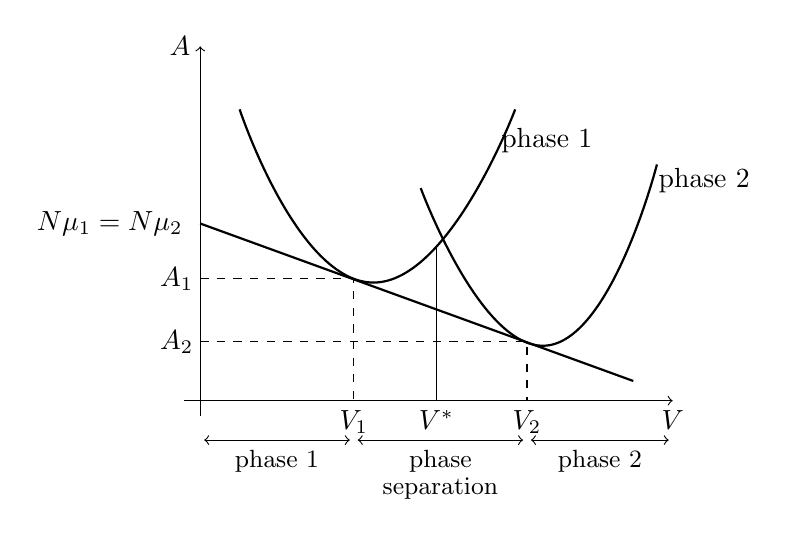
\begin{tikzpicture}
            \draw[->] (-0.2,0)--(6,0)node[below]{\(V\)};
            \draw[->] (0,-0.2)--(0,4.5)node[left]{\(A\)};
            \draw[thick] plot [smooth, tension=1] coordinates { (0.5,3.7) (2.2,1.5) (4,3.7) };
            \draw[thick] plot [smooth, tension=1] coordinates { (2.8,2.7) (4.4,0.7) (5.8,3) };
            \node at (4.4,3.3) {phase 1};
            \node at (6.4,2.8) {phase 2};
            \draw[thick] (0,2.25)--(5.5,0.25);
            \draw[dashed] (0,1.55)--(1.95,1.55)--(1.95,0) node[below]{\(V_1\)};
            \draw[dashed] (0,0.75)--(4.15,0.75)--(4.15,0) node[below]{\(V_2\)};
            \node at (-1.15,2.25){\(N\mu_1=N\mu_2\)};
            \node at (-0.3,1.55) {\(A_1\)};
            \node at (-0.3,0.75) {\(A_2\)};
            \draw (3,1.95)--(3,0)node[below]{\(V^*\)};
            \draw[<->] (0.05,-0.5)--node[below]{\small phase 1}(1.9,-0.5);
            \draw[<->] (2,-0.5)--node[below,align=center]{\small phase \\[-2pt] \small separation}(4.1,-0.5);
            \draw[<->] (4.2,-0.5)--node[below]{\small phase 2}(5.95,-0.5);
        \end{tikzpicture}
    \end{figure}

    If the system is at some volume \(V^*\) with \(V_1\le V^*\le V_2\), the system would have lower Helmholtz energy if it is separated into the two phases than if it exists in either of the single phase. Define \(v\coloneqq V/N\), then
    \begin{equation}
        Nv^*=N_1v_1+(N-N_1)v_2\,.
    \end{equation}
    We can then derive the proportion of particles being in phase 1 at equilibrium
    \begin{equation}
        x_1\coloneqq\frac{N_1}{N}=\frac{v^*-v_2}{v_1-v_2}\,.
    \end{equation}

    Suppose now we have a free energy curve for some phase. We have shown that the free energy must be a convex function of \(V\) because the compressibility \(\kappa\) must be non-negative at equilibrium. Hence, the non-convex part in curve \(A\) versus \(V\) does not correspond to an equilibrium situation. We can still work out the point of coexistence by common tangent construction. But now we have a region where the phase separation is thermodynamically favourable, but the local second derivative of \(A\) with respect to \(V\) is still positive, meaning that any perturbation of such system will increase the free energy. Such a system is described as \textit{metastable} as phase separation will involve a free-energy barrier. Between the inflection points, the free energy curve is non-convex and hence in this range a homogeneous phase would be absolutely unstable, with a negative compressibility. Such a system will phase separate spontaneously under any infinitesimal fluctuation. The boundary between the metastable and unstable regions is called \textit{spinodal}.

    \begin{figure}[ht!]
        \centering
        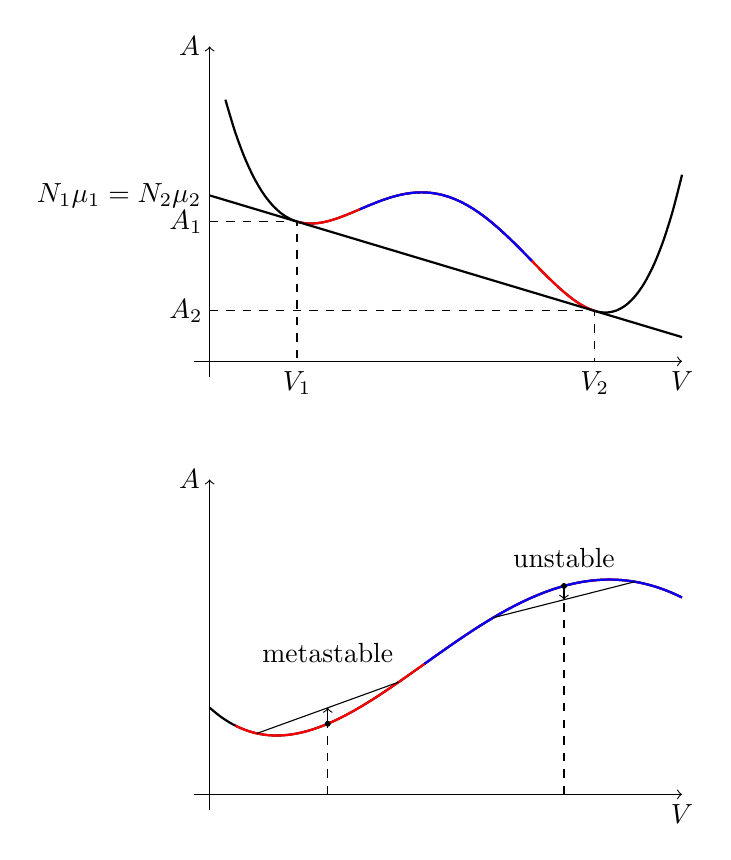
\begin{tikzpicture}
            \draw[->] (-0.2,0)--(6,0)node[below]{\(V\)};
            \draw[->] (0,-0.2)--(0,4)node[left]{\(A\)};
            \draw[thick,domain=0.2:6, smooth, variable=\x,samples=50] plot ({\x}, {3-0.3*\x-0.5*(\x-3)^2 + 0.07*(\x-3)^4});
            \draw[thick,domain=1.11:4.89, red, smooth, variable=\x,samples=50] plot ({\x}, {3-0.3*\x-0.5*(\x-3)^2 + 0.07*(\x-3)^4});
            \draw[thick,domain=1.909:4.091, blue, smooth, variable=\x,samples=50] plot ({\x}, {3-0.3*\x-0.5*(\x-3)^2 + 0.07*(\x-3)^4});
            \draw[thick,domain=0:6, smooth, variable=\x,samples=50] plot ({\x}, {2.107-0.3*\x});
            \draw[dashed] (0,1.774)--(1.11,1.774)--(1.11,0) node[below]{\(V_1\)};
            \draw[dashed] (0,0.64)--(4.89,0.64)--(4.89,0) node[below]{\(V_2\)};
            \node at (-1.15,2.107){\(N_1\mu_1=N_2\mu_2\)};
            \node at (-0.3,1.774) {\(A_1\)};
            \node at (-0.3,0.64) {\(A_2\)};
            
            \begin{scope}[shift={(0,-5.5)}]
                \draw[->] (-0.2,0)--(6,0)node[below]{\(V\)};
                \draw[->] (0,-0.2)--(0,4)node[left]{\(A\)};
                \draw[thick,domain=1:3, smooth, variable=\x,samples=50] plot ({3*\x-3}, {5*(3-0.3*\x-0.5*(\x-3)^2 + 0.07*(\x-3)^4)-8});
                \draw[thick,domain=1.11:3, red, smooth, variable=\x,samples=50] plot ({3*\x-3}, {5*(3-0.3*\x-0.5*(\x-3)^2 + 0.07*(\x-3)^4)-8});
                \draw[thick,domain=1.909:3, blue, smooth, variable=\x,samples=50] plot ({3*\x-3}, {5*(3-0.3*\x-0.5*(\x-3)^2 + 0.07*(\x-3)^4)-8});
                \draw[fill=black] (1.5,0.8969) circle (0.03);
                \draw (0.6,0.7742)--(2.4,1.4258);
                \draw[dashed] (1.5,0)--(1.5,1.1);
                \draw[->] (1.5,0.8969)--(1.5,1.1);
                \draw[fill=black] (4.5,2.6469) circle (0.03);
                \draw (3.6,2.2434)--(5.4,2.7006);
                \draw[dashed] (4.5,0)--(4.5,2.6469);
                \draw[->] (4.5,2.6469)--(4.5,2.472);
                \node at (1.5,1.8) {metastable};
                \node at (4.5,3) {unstable};
            \end{scope}
        \end{tikzpicture}
    \end{figure}

    It should be stressed that the spinodal, although a useful qualitative concept, is not well defined. It appears naturally when we use approximate expressions for the free energy. However, an exact expression for the equilibrium free energy is necessarily convex and therefore has no spinodal.

    \subsubsection{Phase Diagrams}
    A phase diagram can tell us at a glance the conditions under which each phase is thermodynamically stable. For a one-component system, the thermodynamic variables \(P\), \(T\) and \(V\), which are usually used to describe the thermodynamic state of the matter, are not independent of one another. For example, if we specify the volume and the temperature of a system, the pressure will be defined as well through the equation of state. We can therefore think of the phase diagram as a surface in the \(PVT\) space. Such a three-dimensional phase diagram can be projected onto the \(P-T\), \(V-T\), \(P-V\) or \(T-\rho\) planes to give the more familiar two-dimensional phase diagrams.

    There are many other parameters that we could vary; for example we could change the composition of a mixture or the strength of an external magnetic field, and so other types of phase diagrams can be constructed, some of which we shall see in the chapters that follow.
    \subsubsection{Thermodynamic Integration}
    The second law of thermodynamics states that for an isolated system with energy \(E\), volume \(V\) and number of particles \(N\), the entropy \(S\) is maximised when the system is at equilibrium. From this formulation of the second law, it is straightforward to derive the corresponding equilibrium conditions for systems that can exchange heat, particles or volume with a reservoir, as we have already shown. In particular, if a system is in contact with a heat bath, such that its temperature \(T\), volume \(V\) and number of particles \(N\) are fixed, then the Helmholtz energy \(A\coloneqq E-TS\) is at a minimum in equilibrium. Analogously, for a system of \(N\) particles at constant pressure \(P\) and temperature \(T\), the Gibbs energy \(G\coloneqq A+PV\) is at a minimum.

    If we wish to know which of two phases, denoted 1 and 2, is stable at a given temperature and density, we simply need to compare the Helmholtz energies \(A_1\) and \(A_2\). Unfortunately, neither the free energy nor the entropy can be measured directly. What we can measure are averages of \textit{mechanical quantities}, i.e. averages of functions of the coordinates and momenta of the molecules in the system, such as the pressure or the dielectric constant. If we denote such a mechanical quantity by \(X(\{\vb{p}_i\},\{\vb{r}_i\})\), then the average of \(X\) that can be measured in an experiment at constant \(N\), \(V\) and \(T\) is
    \begin{equation}
        \eval{X}_{NVT}=\frac{\int\prod_{i=1}^{N}\dd[3]{\vb{p}_i}\dd[3]{\vb{r}_i}X(\{\vb{p}_i\},\{\vb{r}_i\})\exp[-\beta H(\{\vb{p}_i\},\{\vb{r}_i\})]}{\int\prod_{i=1}^{N}\dd[3]{\vb{p}_i}\dd[3]{\vb{r}_i}\exp[-\beta H(\{\vb{p}_i\},\{\vb{r}_i\})]}\,,
    \end{equation}
    where \(H(\{\vb{p}_i\},\{\vb{r}_i\})\) is the system's Hamiltonian.

    However, the entropy, the free energy and related quantities are not simply averages of functions of the phase-space coordinates of the system. Rather, they are directly related to the volume in phase space that is accessible to a system. For instance, in classical statistical mechanics, the Helmholtz energy \(A\) is directly related to the canonical partition function \(Q(N,V,T)\) through
    \begin{align}
        A&=-k_BT\ln Q(N,V,T)\notag\\
        &=-k_B T\ln\left[\frac{1}{h^{3N}N!}\int\prod_{i=1}^{N}\dd[3]{\vb{p}}\dd[3]{\vb{r}}\exp[-\beta H(\{\vb{p}_i\},\{\vb{r}_i\})]\right]\,.
    \end{align}

    Unlike quantities such as the internal energy, the pressure, or the polarisation, \(Q(N,V,T)\) itself is not a canonical average over the phase space. This is why \(A\) and, for that matter, \(S\) or \(G\), cannot be measured directly. We call quantities that depend directly on the available volume in the phase space \textit{thermal quantities}. However, derivatives of the free energy with respect to the volume \(V\) or the temperature \(T\) are mechanical quantities and can be measured: namely, they are
    \begin{equation}\label{thermal_value_derivatives}
        \left(\pdv{A}{V}\right)_{N,T}=-P\text{ and }\left(\pdv{(A/T)}{(1/T)}\right)_{N,V}=E\,.
    \end{equation}
    In order to compute the free energy of a system at a given temperature and density, we must find a reversible path in the volume-temperature plane that links the state under consideration to a state of known free energy. The change in \(A\) along that path can then simply be evaluated by integrating (\ref{thermal_value_derivatives}). Only a few thermodynamic states exist whose free energy is known exactly: one such state is the ideal gas; another may be perfectly ordered ground state at \(T=0\unit{K}\).

    \subsection{Gibbs--Bogoliubov Inequality}
    The aim of thermodynamic perturbation theory is to arrive at an estimate of the free energy (and all derived properties) of a many-body system, using as input information about the free energy and structure of a simpler reference system. We assume that the potential energy function of this reference system is denoted by \(U_0\), while the potential energy function of the system of interest is denoted by \(U_1\). In order to compute the free-energy difference between the known reference system and the system of interest, we use a linear parameterisation of the potential energy function
    \begin{equation}
        U(\lambda)\coloneqq \lambda U_1+(1-\lambda)U_0\,.
    \end{equation}
    The free energy of a system with this generalised potential energy is denoted \(A(\lambda)\) and can be computed from \(A(\lambda)=-k_B T\ln Q(\lambda)\). In particular, we noted when introducing (\ref{thermal_value_derivatives}) that derivatives of the free energy are often mechanical observables, and the same applies in this case. The derivative of \(A(\lambda)\) with respect to \(\lambda\) is
    \begin{align}
        \left(\pdv{A}{\lambda}\right)_{N,V,T}&=\frac{\int\prod_{i=1}^{N}\dd[3]{\vb{r}_i}\left(\pdv{U(\{\vb{r}_i\};\lambda)}{\lambda}\right)\exp[-\beta U(\{\vb{r}_i\};\lambda)]}{\int\prod_{i=1}^{N}\dd[3]{\vb{r}_i}\exp[-\beta U(\{\vb{r}_i\};\lambda)]}\notag\\
        &=\eval{\pdv{U(\lambda)}{\lambda}}_{\lambda}\notag\\
        &=\eval{U_1-U_0}_\lambda\,,
    \end{align}
    and hence we can express the free-energy difference \(A_1-A_0\) as
    \begin{equation}
        A_1-A_0=\int_{0}^{1}\dd{\lambda}\eval{U_1-U_0}_\lambda\,,
    \end{equation}
    where the subscript \(\lambda\) indicates that we evaluate the thermal average at that value of \(\lambda\). This expression, first derived by John Kirkwood in 1935, allows us to compute the free energy of a system of interest by relating it to a reference system. This approach has been used extensively in computer simulations since the mid-1980s. It is often referred to as `artificial' or `Hamiltonian' thermodynamic integration because it entails changing the underlying interactions in the system's Hamiltonian.

    Moreover, it allows us to find bounds on the free energy \(A_1\). It is straightforward to show that
    \begin{equation}
        \left(\pdv[2]{A}{\lambda}\right)_{N,V,T}=-\beta\left(\eval{(U_1-U_0)^2}_\lambda-\eval{U_1-U_0}_\lambda^2\right)\le 0\,.
    \end{equation}
    Since the right-hand side of the equation is the negative of a variance, we can note that the second derivative of \(A\) with respect to \(\lambda\) is always non-positive. This implies that
    \begin{equation}
        \left(\pdv{A}{\lambda}\right)_{\lambda=0}\ge\left(\pdv{A}{\lambda}\right)_{\lambda>0}\,,
    \end{equation}
    and hence
    \begin{equation}\label{Gibbs_Bogoliubov}
        A_1\le A_0+\eval{U_1-U_0}_{\lambda=0}\,.
    \end{equation}
    This variational principle for the free energy is known as the \textit{Gibbs--Bogoliubov inequality}: we compute an upper bound to the free energy of the system of interest from a knowledge of the average of \(U_1-U_0\) evaluated for the reference system. The latter is something that can often be computed because the reference system is by construction a system which we can solve.

    \begin{figure}[ht!]
        \centering
        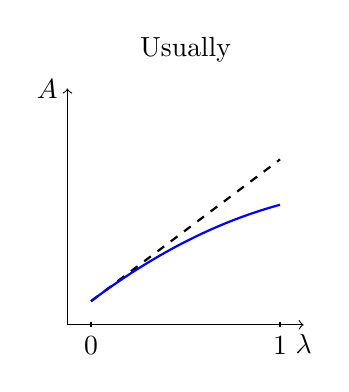
\begin{tikzpicture}
            \draw[->] (0,0)--(3,0)node[below]{\(\lambda\)};
            \draw (0.3,0.03)--(0.3,-0.03)node[below]{\(0\)};
            \draw (2.7,0.03)--(2.7,-0.03)node[below]{\(1\)};
            \draw[->] (0,0)--(0,3)node[left]{\(A\)};
            \draw[dashed,thick] (0.3,0.3)--(2.7,2.1);
            \draw[thick,domain=0.3:2.7, blue, smooth, variable=\x,samples=50] plot ({\x}, {0.75*\x+0.075-0.1*(\x-0.3)^2});
            \node at (1.5,3.5) {Usually};
        \end{tikzpicture}
        \begin{tikzpicture}
            \draw[->] (0,0)--(3,0)node[below]{\(\lambda\)};
            \draw (0.3,0.03)--(0.3,-0.03)node[below]{\(0\)};
            \draw (2.7,0.03)--(2.7,-0.03)node[below]{\(1\)};
            \draw[->] (0,0)--(0,3)node[left]{\(A\)};
            \draw[blue,thick] (0.3,0.3)--(2.7,2.1);
            \node at (1.5,3.5) {Sometimes};
        \end{tikzpicture}
        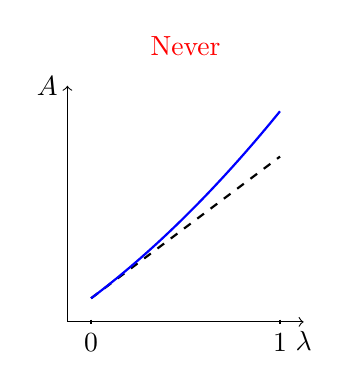
\begin{tikzpicture}
            \draw[->] (0,0)--(3,0)node[below]{\(\lambda\)};
            \draw (0.3,0.03)--(0.3,-0.03)node[below]{\(0\)};
            \draw (2.7,0.03)--(2.7,-0.03)node[below]{\(1\)};
            \draw[->] (0,0)--(0,3)node[left]{\(A\)};
            \draw[dashed,thick] (0.3,0.3)--(2.7,2.1);
            \draw[thick,domain=0.3:2.7, blue, smooth, variable=\x,samples=50] plot ({\x}, {0.75*\x+0.075+0.1*(\x-0.3)^2});
            \node at (1.5,3.5)[red]{Never};
        \end{tikzpicture}
        \caption{The Gibbs--Bogoliubov inequality shows that the first-order perturbation estimation of the free energy is never lower than the true free energy.}
    \end{figure}

    We may let our reference system depend on some parameters and use the variational principle to get our best estimation of the upper bound of Helmholtz energy.

    It may seem at first glance that we are doing something slightly odd here: what does it actually mean that we compute \(\eval{U_1}_{\lambda=0}\) for the reference potential, given that when \(\lambda=0\), the system is governed by \(U_0\) only? In this case, \(U_1\) does not contribute to the Boltzmann factor, but that does not mean we are not able to compute what it is for a given microstate. This is similar to computing any other mechanical observable, e.g. the pressure, which also would not appear in the Boltzmann factor. It is evaluated as
    \begin{equation}
        \eval{U_1-U_0}_{\lambda=0}=\frac{\int\prod_{i=1}^{N}\dd[3]{\vb{r}_i}(U_1-U_0)\exp(-\beta U_0)}{\int\prod_{i=1}^{N}\dd[3]{\vb{r}_i}\exp(-\beta U_0)}\,.
    \end{equation}

    The usefulness of (\ref{Gibbs_Bogoliubov}) depends crucially on the quality of the choice of reference system. A good reference system is not necessarily close in free energy to the system of interest, but one for which the fluctuation in the potential energy difference \(U_1-U_0\) are small. Thermodynamic perturbation theory for simple liquids has been very successfully precise because the structure of the reference system (hard-sphere fluid) and the liquid under consideration (e.g. Lennard-Jones) are very similar. As a result, \(\eval{U_1-U_0}_{\lambda}\) hardly depends on \(\lambda\) and so its derivative is small.

    \subsection{Mean-Field Theory and the Ising Model}
    The Gibbs--Bogoliubov inequality can be used as a starting point from which we can derive mean-field theory, which provides a systematic approximation to the free energy of a many-body system. Let's start with a seemingly simple yet interesting and arguably the most important model in statistical mechanics and related fields --- the Ising model. The Ising model describes the magnetism of materials by considering spins on a lattice with Hamiltonian
    \begin{equation}
        U_1=-\frac{J}{2}\sum_{i=1}^{N}\sum_{\langle i,j\rangle}s_is_j-B\sum_{i=1}^{N}s_i\,,
    \end{equation}
    where \(\langle i,j\rangle\) indicates that the particle \(j\) is one of the nearest neighbours of \(i\) and the factor of \(1/2\) ensures that we do not double count the interactions. \(B\) is the external magnetic field, which we will now set to be zero. The Ising model is not just relevant for magnetic systems; in appendix \cref{Chap:Ising_Lattice_Gas}, we show that a lattice-gas model that can be used to describe the liquid-vapour transition is actually equivalent to the Ising model.

    \begin{figure}
        \centering
        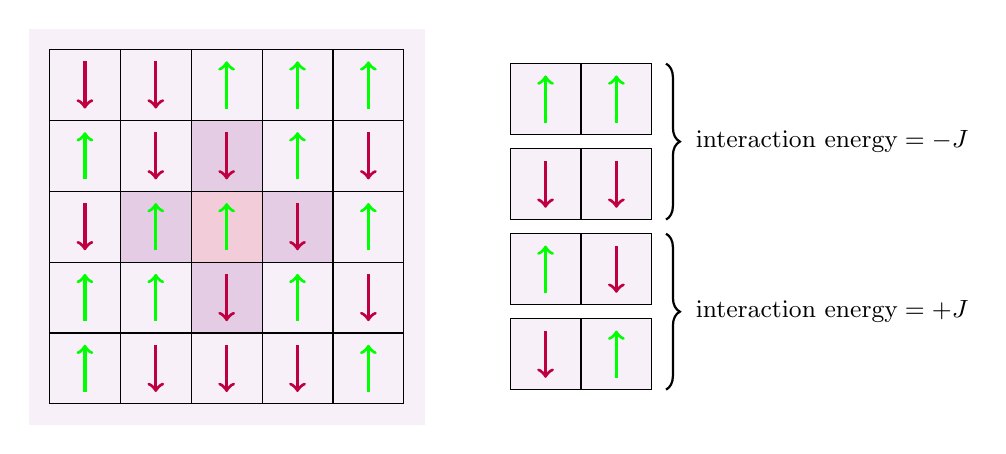
\begin{tikzpicture}[scale=0.9]
            \pgfmathsetseed{2}

            \draw[white, fill=blue!5!violet!6] (-2.8,-2.8) rectangle (2.8,2.8);

            \foreach \x in {-3,...,2}{
                \draw (0.5+\x,-2.5)--(0.5+\x,2.5);
                \draw (-2.5,0.5+\x)--(2.5,0.5+\x);
            }

            \draw[fill=violet!20] (-0.5,-1.5) rectangle (0.5,1.5);
            \draw[fill=violet!20] (-1.5,-0.5) rectangle (1.5,0.5);
            \draw[fill=purple!20] (-0.5,-0.5) rectangle (0.5,0.5);

            \foreach \i in {-2,...,2}{
                \foreach \j in {-2,...,2}{
                    \pgfmathrandominteger{\a}{1}{2}
                    \ifthenelse{\a = 1}{\node at (\i,\j) {\up};}{\node at (\i,\j) {\down};}
                }
            }

            \foreach \x in {0,...,3}{
                \draw[fill=blue!5!violet!6] (4,1.2*\x-2.3) rectangle (5,1.2*\x-1.3);
                \draw[fill=blue!5!violet!6] (6,1.2*\x-2.3) rectangle (5,1.2*\x-1.3);
            }

            \node at (4.5,1.8) {\up};
            \node at (5.5,1.8) {\up};
            \node at (4.5,0.6) {\down};
            \node at (5.5,0.6) {\down};
            \node at (4.5,-0.6) {\up};
            \node at (5.5,-0.6) {\down};
            \node at (4.5,-1.8) {\down};
            \node at (5.5,-1.8) {\up};

            \draw [decorate,decoration={brace,amplitude=5pt,mirror},thick] (6.2,0.1) -- (6.2,2.3) node[midway,xshift=6em]{\small \(\text{interaction energy}=-J\)};
            \draw [decorate,decoration={brace,amplitude=5pt,mirror},thick] (6.2,-2.3) -- (6.2,-0.1) node[midway,xshift=6em]{\small \(\text{interaction energy}=+J\)};
        \end{tikzpicture}
        \caption{A schematic representation of the Ising model in two dimensions.}
    \end{figure}

    We wish to approximate this model system using a reference system with a much simpler Hamiltonian, namely one that consists only of a sum of one-particle contributions. For example,
    \begin{equation}
        U_0=-\sum_{i=1}^{N}hs_i\,,
    \end{equation}
    where \(h\) denotes the effective field that replaces the interaction with the other particles. The molecular partition function counting all states of a single spin (with energy \(-hs\)) in the reference system is
    \begin{equation}
        q_0=\int\dd{s}\exp(\beta hs)
    \end{equation}
    and the free energy per spin is
    \begin{equation}
        a_0(h)=-k_BT\ln q_0=-k_BT\ln\int\dd{s}\exp(\beta hs)\,.
    \end{equation}
    Here, we use the shorthand \(a\) for \(A/N\). If the spins are quantised and we only have two spin states (\(+1\) and \(-1\)), the partition function reduces to
    \begin{equation}
        q_0=\exp(\beta h)+\exp(-\beta h)=2\cosh(\beta h)
    \end{equation}
    and the free energy becomes
    \begin{equation}
        a_0(h)=-k_BT\ln(2\cosh(\beta h))\,.
    \end{equation}
    We can easily compute the average value of \(s\) in the reference system,
    \begin{equation}
        \eval{s}_0=\frac{\int\dd{s}s\exp(\beta hs)}{q_0}=\frac{1}{q_0}\pdv{}{\beta h}\int\dd{s}\exp(\beta hs)=k_B T\pdv{\ln q_0}{h}\,,
    \end{equation}
    or simply
    \begin{equation}
        \eval{s}_0=-\pdv{a_0(h)}{h}\,.
    \end{equation}
    In the case of spins \(\pm 1\),
    \begin{equation}\label{Ising_average_spin}
        \eval{s}_0=\tanh(\beta h)\,,
    \end{equation}
    which we could have obtained directly from the definition of the mean magnetisation, but the expression involving the derivative of \(a_0\) will come in useful shortly. Now, we consider the Gibbs--Bogoliubov inequality, where
    \begin{align}
        a_{\text{MF}}&=a_0+\eval{-\frac{J}{2}\sum_{\langle i,j\rangle}s_is_j+hs_i}_0\notag\\
        &=a_0-\frac{J}{2}z\eval{s}_0^2+h\eval{s}_0\,.\label{Ising_free_energy}
    \end{align}
    In the last line, we have introduced \(z\), the coordination number of particle \(i\). Moreover, we have used the fact that, in the reference system, different spins are uncorrelated, \(\eval{s_is_j}_0=\eval{s_i}_0\eval{s_j}_0\). We now look for the optimum value of \(h\), i.e. the one that minimises our estimate of \(a_{\text{MF}}\). Carrying out the differentiation with respect to \(h\), we find that
    \begin{align}
        0&=\pdv{}{h}\left(a_0-\frac{J}{2}z\eval{s}_0^2+h\eval{s}_0\right)\notag\\
        &=-\eval{s}_0-(Jz\eval{s}_0-h)\pdv{\eval{s}_0}{h}+\eval{s}_0\notag\\
        &=-(Jz\eval{s}_0-h)\pdv{\eval{s}_0}{h}\,.
    \end{align}
    Since \(\pdv{\eval{s}_0}{h}\ne 0\), we can conclude that
    \begin{equation}\label{Ising_mean_field_strength}
        h=Jz\eval{s}_0\,.
    \end{equation}
    Finally, we can insert this expression for \(h\) into (\ref{Ising_average_spin}) to obtain an implicit equation for \(\eval{s}_0\),
    \begin{equation}\label{Ising_equilibrium_condition}
        \eval{s}_0=\tanh(\beta Jz\eval{s}_0)\,,
    \end{equation}
    which can be solved to yield \(\eval{s}_0\) as a function of \(T\).

    \begin{figure}
        \centering
        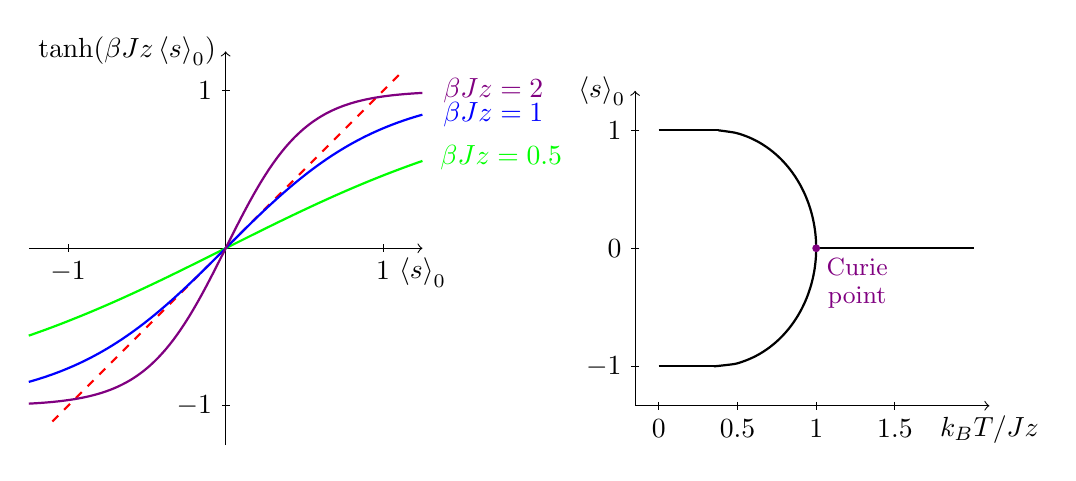
\begin{tikzpicture}
            \draw[->] (-2.5,0)--(2.5,0)node[below]{\(\eval{s}_0\)};
            \draw[->] (0,-2.5)--(0,2.5)node[left]{\(\tanh(\beta Jz\eval{s}_0)\)};
            \draw (2,0.05)--(2,-0.05)node[below]{\(1\)};
            \draw (-2,0.05)--(-2,-0.05)node[below]{\(-1\)};
            \draw (0.05,2)--(-0.05,2)node[left]{\(1\)};
            \draw (0.05,-2)--(-0.05,-2)node[left]{\(-1\)};
            \draw[dashed,thick,red] (-2.2,-2.2)--(2.2,2.2);
            \draw[thick,domain=-1.25:1.25, green, smooth, variable=\x,samples=50] plot ({2*\x}, {2*(2.72^(0.5*\x)-2.72^(-0.5*\x))/(2.72^(0.5*\x)+2.72^(-0.5*\x))});
            \draw[thick,domain=-1.25:1.25, blue, smooth, variable=\x,samples=50] plot ({2*\x}, {2*(2.72^(\x)-2.72^(-\x))/(2.72^(\x)+2.72^(-\x))});
            \draw[thick,domain=-1.25:1.25, violet, smooth, variable=\x,samples=50] plot ({2*\x}, {2*(2.72^(2*\x)-2.72^(-2*\x))/(2.72^(2*\x)+2.72^(-2*\x))});
            \node at (3.5,1.15)[green]{\(\beta Jz=0.5\)};
            \node at (3.4,1.7)[blue]{\(\beta Jz=1\)};
            \node at (3.4,2)[violet]{\(\beta Jz=2\)};

            \draw[->] (5.2,-2)--(9.7,-2)node[below]{\(k_BT/Jz\)};
            \draw[->] (5.2,-2)--(5.2,2)node[left]{\(\eval{s}_0\)};
            \draw (5.5,-1.95)--(5.5,-2.05)node[below]{\(0\)};
            \draw (6.5,-1.95)--(6.5,-2.05)node[below]{\(0.5\)};
            \draw (7.5,-1.95)--(7.5,-2.05)node[below]{\(1\)};
            \draw (8.5,-1.95)--(8.5,-2.05)node[below]{\(1.5\)};
            \draw (5.25,-1.5)--(5.15,-1.5)node[left]{\(-1\)};
            \draw (5.25,0)--(5.15,0)node[left]{\(0\)};
            \draw (5.25,1.5)--(5.15,1.5)node[left]{\(1\)};
            \draw[thick] (5.5,1.5)--(6.26,1.5);
            \draw[thick] (5.5,-1.5)--(6.2,-1.5);
            \draw[thick,domain=-1.5:1.5, smooth, variable=\y,samples=100] plot ({6.2+(1.5^2-\y*\y)^(0.5)*1.3/1.5}, {\y});
            \draw[thick] (7.5,0)node[below right,violet,align=center]{\small Curie \\[-2pt] \small point}--(9.5,0);
            \fill[violet] (7.5,0) circle (0.05);
        \end{tikzpicture}
        \caption{(a) A graphical method for the solution of the mean magnetisation in Ising model. (b) The phase diagram of an Ising model system.}
    \end{figure}

    Above the \textit{critical} (or \textit{Curie}) \textit{temperature} \(k_B T=Jz\), there is only one solution \(\eval{s}_0=0\): at high temperatures, the entropy dominates the free energy and so the spins are randomly distributed. The significance of the entropy as a driving force is diminished as the temperature is decreased, and below the Curie temperature, the net alignment of spins, which is energetically favourable, becomes dominant, and we get two extra solutions with non-zero mean magnetisation. Amongst all the three solutions, the \(\eval{s}_0=0\) solution is actually a maximum rather than a minimum so we will ignore it. In the absence of an external magnetic field, the system is equally likely to be magnetised in the up or the down spin configurations, but the fluctuations causing the transitions between the two are extremely unlikely. The ergodic hypothesis\footnote{Being \textit{ergodic} means that a point (the state of the system in this case) will eventually visit all parts of the space (the phase space) as it evolves over time, in a uniform and random sense.} is thus formally violated, and this phenomenon is sometimes described as \textit{spontaneous symmetry breaking}.

    The free energy estimate that we obtain when inserting (\ref{Ising_mean_field_strength}) into (\ref{Ising_free_energy}) is
    \begin{equation}\label{Ising_MF_free_energy}
        a_{\text{MF}}=a_0+\frac{J}{2}z\eval{s}_0^2\,.
    \end{equation}
    The subscript `MF' in this expression stands for the mean field approximation. It is very important to bear in mind that the free energy that results from the mean-field approximation is in general not simply the free energy of the reference system with the effective field, but has an additional term that depends on the difference between the two potentials measured for the system with the effective field.
    \subsubsection{Validity of Mean Field Theory}
    Having solved the Ising model using mean field theory, a question that arises is: are our results correct?

    There is actually a version of the Ising model for which the mean field theory is exact: it is the \(d=\infty\) dimensional lattice. This is unphysical. Roughly speaking, mean field theory works for large \(d\) because each spin has a large number of neighbours and so indeed sees something close to the average spin.
    
    But what about dimensions of interest? Mean field theory gets things most dramatically wrong in \(d=1\). In that case, no phase transition actually occurs. We will solve the 1D Ising model exactly in the appendix \cref{Chap:Exact_Ising}. There is a general lesson here: in low dimensions, both thermal and quantum fluctuations are more important and invariably stop systems forming ordered phases.

    In higher dimensions, \(d\ge 2\), the crude features of the phase diagram, including the existence of a phase transition, given by mean field theory are essentially correct. In fact, the very existence of a phase transition is already worthy of comment. The defining feature of a phase transition is behaviour that jumps discontinuously as we vary \(\beta\). Mathematically, the functions must be non-analytic. Yet all properties of the theory can be extracted from the partition function \(Q\) which is a sum of smooth, analytic exponential functions
    \begin{equation}
        Q=\sum_{\ket{i}}\ee^{-\beta E_i}\,.
    \end{equation}
    How can we get a phase transition? The loophole is that \(Q\) is only necessarily analytic if the sum is finite. But there is no such guarantee when the number of lattice sites \(N\to\infty\). We reach a conclusion: phase transitions only strictly happen in the thermodynamic limit. There are no phase transitions in finite systems.

    The 2D Ising model in a square lattice has been solved exactly, first by Onsager --- his method was famously complicated. In appendix \cref{Chap:Exact_Ising}, we will use a clever trick to obtain the exact result of critical temperature, which is
    \begin{equation}
        k_B T=\frac{2J}{\ln(\sqrt{2}+1)}\approx 2.269J\,.
    \end{equation}
    This is actually not hugely different from the mean field approximation, which predicts
    \begin{equation}
        k_B T=Jz=4J\,.
    \end{equation}

    \begin{figure}
        \centering
        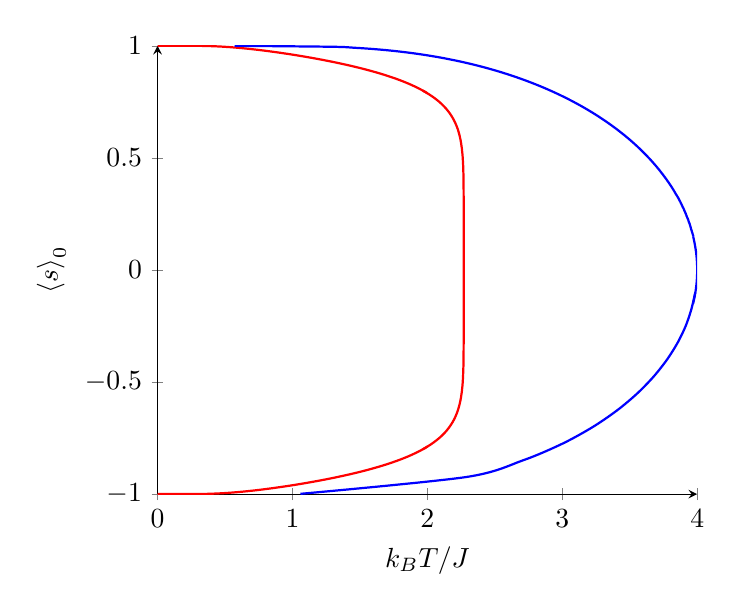
\begin{tikzpicture}
            \begin{axis}[
                axis lines = left,
                xlabel = \(k_B T/J\),
                ylabel = {\(\eval{s}_0\)},
            ]
                \addplot [
                    domain=0:2, 
                    samples=200,
                    color=red,
                    thick,smooth
                ]
                {(1-2/(exp(2/x)-exp(-2/x)))^(0.125)};
                \addplot [
                    domain=0:2, 
                    samples=200, 
                    color=red,
                    thick,smooth
                ]
                {-(1-2/(exp(2/x)-exp(-2/x)))^(0.125)};
                \addplot [
                    domain=-0.8:0.8, 
                    samples=200, 
                    color=red,
                    thick,smooth
                ]
                ({2/(ln(1/(1-x^8)+sqrt((1/(1-x^8))^2+1)))},{x});
                \addplot [
                    domain=-15:-0.1, 
                    samples=200, 
                    color=blue,
                    thick,smooth
                ]
                ({8*x/ln((1+x)/(1-x))},{x});
                \addplot [
                    domain=0.15:1, 
                    samples=200, 
                    color=blue,
                    thick,smooth
                ]
                ({8*x/ln((1+x)/(1-x))},{x});
                \addplot [
                    domain=-0.15:0.15, 
                    samples=100, 
                    color=blue,
                    thick,smooth
                ]
                ({4-4*x^2/3-16*x^4/45-176*x^6/945},{x});
            \end{axis}
        \end{tikzpicture}
        \caption{Mean magnetisation of the exact (red) and the mean field (blue) 2D square lattice Ising model.}
    \end{figure}

    \subsection{Liquid-Gas Phase Transition}
    Now we will investigate probably the most common phase transition --- liquid-gas phase transition. We will take a hard-sphere gas as a reference system and add a very weak, attractive interaction \(-\epsilon\) that extends to a very large distance \(R_c\). This crude model leads to the famous van der Waals equation of state.

    \begin{figure}
        \centering
        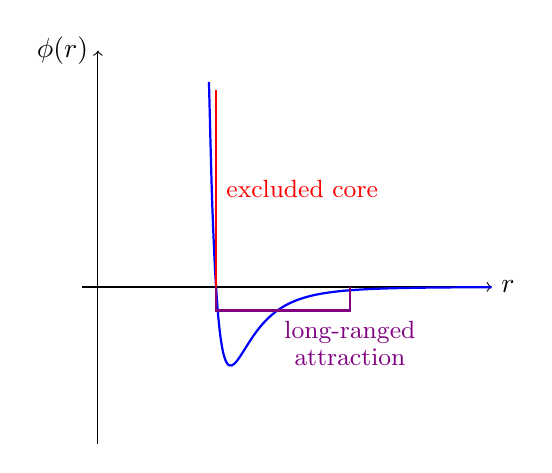
\begin{tikzpicture}
            \draw[->] (-0.2,0)--(5,0)node[right]{\(r\)};
            \draw[->] (0,-2)--(0,3)node[left]{\(\phi(r)\)};
            \draw[thick,domain=1.41:5, smooth, variable=\x,samples=100,blue] plot ({\x}, {4*((1.5/\x)^12 - (1.5/\x)^6)});
            \draw[thick,red] (1.5,0)--node[right]{\small excluded core}(1.5,2.5);
            \draw[thick,violet] (1.5,0)--(1.5,-0.3)--(3.2,-0.3)node[below,align=center]{\small long-ranged \\[-2pt] \small attraction}--(3.2,0);
        \end{tikzpicture}
        \caption{A typical interatomic potential (shown in blue) can be approximated by a hard-core repulsion and a very weak attractive interaction \(-\epsilon\).}
    \end{figure}

    \subsubsection{Hard-Sphere Gas}
    The hard-sphere potential is given by
    \begin{equation}
        U_0=\sum_{i<j}\phi(r_{ij})\,,
    \end{equation}
    where
    \begin{equation}
        \phi(r_{ij})=\begin{cases}
            0 & \text{if }r_{ij}>\sigma\\
            \infty & \text{if }r_{ij}\le\sigma\,,
        \end{cases}
    \end{equation}
    where \(\sigma\) is the diameter of the particle.

    Provided the hard-sphere gas is sufficiently dilute, we can estimate that the addition of each additional hard sphere reduces the volume available to the next one by \(v_{\text{ex}}=4\pi\sigma^3/3\), the volume excluded by a single hard sphere. In the dilute limit, we estimate that no two excluded volumes will overlap. An illustration of this set-up is given in the figure below. In this case, we can simply modify the perfect gas partition function to give
    \begin{align}
        Q_{\text{HS}}&\approx\frac{1}{\Lambda^{3N}N!}V(V-v_{\text{ex}})(V-2v_{\text{ex}})\dots(V-(N-1)v_{\text{ex}})\notag\\
        &=\frac{V^N}{\Lambda^{3N}N!}\left(1-\frac{v_{\text{ex}}}{V}\right)\left(1-2\frac{v_{\text{ex}}}{V}\right)\dots\left(1-(N-1)\frac{v_{\text{ex}}}{V}\right)\,.
    \end{align}
    \begin{figure}[ht!]
        \centering
        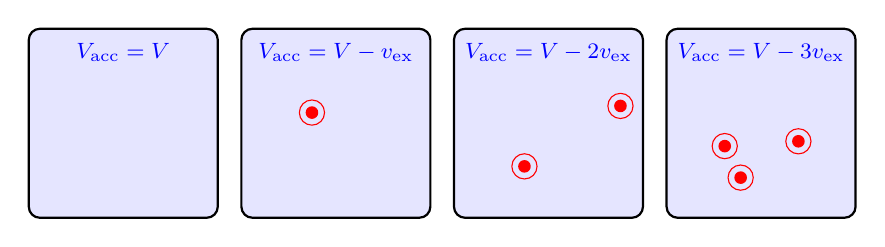
\begin{tikzpicture}
            \foreach \i in {0,...,3}{
                \draw[rounded corners, fill=blue!10, thick] (2.7*\i,-1.2) rectangle (2.7*\i+2.4,1.2);
            }
            \node at (1.2,0.9)[blue]{\footnotesize\(V_{\text{acc}}=V\)};
            \node at (3.9,0.9)[blue]{\footnotesize\(V_{\text{acc}}=V-v_{\text{ex}}\)};
            \node at (6.6,0.9)[blue]{\footnotesize\(V_{\text{acc}}=V-2v_{\text{ex}}\)};
            \node at (9.3,0.9)[blue]{\footnotesize\(V_{\text{acc}}=V-3v_{\text{ex}}\)};

            \pgfmathsetseed{1}
            \foreach \num in {1,2,3}{
                \begin{scope}[shift = {(2.7*\num,0)}]
                    \foreach \i in {1,...,\num}{
                        \tikzmath{
                            \x = rand + 1.2;
                            \y = rand;
                        }
                        \fill [red] (\x,\y) circle (0.08);
                        \draw [red] (\x,\y) circle (0.16);
                    }
                \end{scope}
            }
        \end{tikzpicture}
        \caption{Ignoring any volume excluded by the walls and any excluded volume overlaps, each particle inserted into the system excludes a volume \(v_{\text{ex}}\), reducing the accessible volume.}
    \end{figure}
    
    In the dilute regime, \((N-1)v_{\text{ex}}/V\ll 1\), so we can use the power series \(\exp(-x)=1-x\), giving
    \begin{align}
        Q_{\text{HS}}&=\frac{V^N}{\Lambda^{3N}N!}\exp\left(-\frac{v_{\text{ex}}}{V}\right)\exp\left(-\frac{2v_{\text{ex}}}{V}\right)\dots\exp\left(-\frac{(N-1)v_{\text{ex}}}{V}\right)\notag\\
        &=\frac{V^N}{\Lambda^{3N}N!}\exp\left(-\frac{v_{\text{ex}}}{V}\sum_{i=1}^{N-1}i\right)\,.
    \end{align}
    The summation is an arithmetic series that we can evaluate as \(N(N-1)/2\). Since \(Nv_{\text{ex}}/2V\ll 1\) by construction, we can ignore the term linear in \(N\) in the exponent and write
    \begin{equation}
        Q_{\text{HS}}\approx\frac{V^N}{\Lambda^{3N}N!}\exp\left(-\frac{N^2v_{\text{ex}}}{2V}\right)=\frac{V^N}{\Lambda^{3N}N!}\left[\exp\left(-\frac{Nv_{\text{ex}}}{2V}\right)\right]^N\,.
    \end{equation}
    If we use the same expansion again and if we note that \(v_{\text{ex}}=8v_0\), where \(v_0\) is the volume of a single hard sphere particle, we obtain
    \begin{equation}
        Q_{\text{HS}}\approx\frac{(V-4Nv_0)^N}{\Lambda^{3N}N!}\,.
    \end{equation}
    Using \(A=-k_B T\ln Q\), Stirling's approximation and \(P=-(\pdv{A}{V})_{N,T}\), we can write
    \begin{equation}
        P_{\text{HS}}\approx\frac{Nk_BT}{V-4Nv_0}=\frac{k_B T}{v_0}\frac{\phi}{1-4\phi}\,,
    \end{equation}
    where in the last step we rewrote the volume in terms of the overall fraction of volume occupied, \(\phi\coloneqq Nv_0/V\). We note that this function diverges when \(\phi\to 1/4\). In reality, hard spheres can be compressed to the close-packed volume fraction \(\phi=\pi/\sqrt{18}\approx 0.7405\), and so the approximate partition function above is not appropriate at higher densities. This hard-sphere equation of state, and the corresponding van der Waals equation of state that we will derive from it, are thus approximations that are only reasonable at low density.
    \subsubsection{Mean-Field Attractions}
    We have accounted for, in an approximated way, the hard-core repulsion between particles. We would now like to add the weak pairwise attraction \(-\epsilon\). In particular, we consider the limit of very weak attractions (\(\epsilon\to 0\)) that are very long-range (\(R_c\to\infty\)). In this limit, the potential energy of the perturbed fluid can be computed directly. Within a shell of radius \(R_c\), there will be, on average, \(N_c=(4/3)\pi R_c^3\rho\) other particles, where \(\rho\) is the number density of the fluid. All these particles contribute \(-\epsilon/2\) to the potential energy of the fluid, with the factor of \(1/2\) accounting for the double-counting of pairwise interaction. For \(R_c\to\infty\), the number of neighbours \(N_c\) also tends to infinity and hence the relative fluctuation in \(N_c\) becomes negligible, as it is of order \(1/\sqrt{N_c}\). It then follows that the fluctuation in the perturbation (i.e. \(U_1-U_0\)) also becomes negligible and, since we have shown that the second derivative of the free energy is proportional to the variance in \(U_1-U_0\), the first-order Maclaurin expansion of the free energy in \(\lambda\) becomes exact. Therefore the Gibbs--Bogoliubov inequality becomes an identity. The free energy per particle of the van der Waals fluid is therefore
    \begin{equation}
        \left(\frac{A}{N}\right)_{\text{vdW}}(\rho,T)=\left(\frac{A}{N}\right)_{\text{HS}}(\rho,T)-\rho a\,,
    \end{equation}
    where we have defined \(a=(2\pi/3)R_c^3\epsilon\). The corresponding pressure is
    \begin{equation}
        P_{\text{vdW}}=-\left(\pdv{A_{\text{vdW}}}{V}\right)_{N,T}=\rho^2\pdv{(A/N)_{\text{vdW}}}{\rho}=P_{\text{HS}}(\rho,T)-a\rho^2\,,
    \end{equation}
    where \(P_{\text{HS}}\) denotes the pressure of the hard-sphere reference system. We therefore have the well-known van der Waals equation
    \begin{equation}
        (P_{\text{vdW}}+a\rho^2)(V-Nb)=Nk_B T\,,
    \end{equation}
    where \(b=4v_0\). This equation is very interesting to study because it is probably the simplest model system which exhibits vapour-liquid coexistence. A simple way of computing the phase diagram involves the use of Maxwell's equal-area construction.
    \subsubsection{Maxwell Equal-Area Construction}
    We can sketch the behaviour of the pressure with volume above and below the critical point. Above the critical point, a single fluid phase exists; below the critical point, a vapour (low-density fluid) and a liquid (high-density fluid) are predicted. Below the critical point, there are regions where the equation of state describes a mechanically unstable state where the isothermal compressibility is negative, and where a single pressure corresponds to multiple possible volumes. Such regions are known as van der Waals loops. The critical point itself occurs at the point at which the minimum and the maximum of the van der Waals loop merge, i.e. the first and second derivatives of the pressure with respect to volume vanish.

    In regions where there are van der Waals loops, we can immediately find the points corresponding to limits of mechanical stability: these spinodals correspond to the points at which (\(\partial P/\partial V\)) changes sign. Finding the points of coexistence (the \textit{binodals}) is slightly more challenging. Various approaches can be used; here, we will use a method called Maxwell construction.

    We have already shown that the condition for phase equilibrium --- in this case between the liquid and the vapour --- is the equality of pressures, temperatures and chemical potentials. From our discussion of the common tangent construction approach, we know that the condition that the chemical potentials are equal is given by
    \begin{equation}
        N\mu_1=N\mu_2=A_1+P_{\text{comm}}V_1=A_2+P_{\text{comm}}V_2\,,
    \end{equation}
    where \(P_{\text{comm}}\) is the common pressure. This is fulfilled if \(P_{\text{comm}}(V_1-V_2)=A_1-A_2\).

    We can also express the pressure as \(P=-(\partial A/\partial V)_{N,T}\), and therefore, if we use thermodynamic integration, we find that
    \begin{equation}
        A_1-A_2=-\int_0^{V_1}\dd{V}P+\int_{0}^{V_2}\dd{V}P\,.
    \end{equation}
    Hence the condition for coexistence is
    \begin{equation}\label{Maxwell_equal_area}
        P_{\text{comm}}(V_2-V_1)=\int_{V_1}^{V_2}\dd{V}P\,.
    \end{equation}
    This condition means that the area of the rectangle spanned by \(V_1\) and \(V_2\) along the volume axis and 0 and \(P_{\text{comm}}\) along the pressure axis is equal to the area under the \(P\) curve between \(V_1\) and \(V_2\). As can be seen in the figure, the only difference between the two areas is the region where area 1 carves an area
    into the rectangle and area 2 protrudes from the rectangle: to satisfy (\ref{Maxwell_equal_area}), we simply require that area 1 should equal area 2. In practice, we need to vary \(P_{\text{comm}}\) until the two areas match. A phase diagram corresponding to the van der Waals equation of state is shown in the figure.

    \begin{figure}
        \centering
        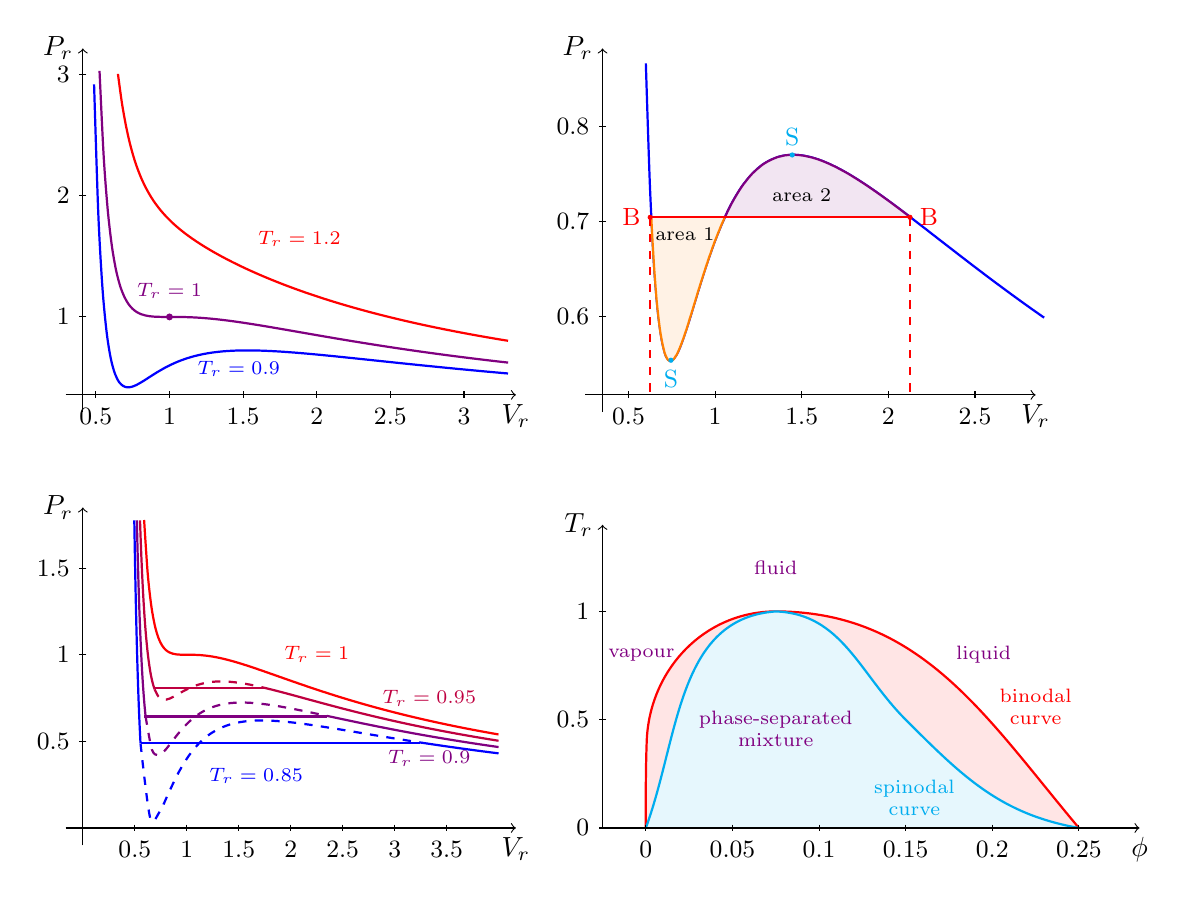
\begin{tikzpicture}[scale=1.1]
            \draw[->](-0.2,0) -- (5,0) node[below]{\(V_r\)};
            \draw[->](0,-0.2) -- (0,4) node[left]{\(P_r\)};
            \draw[red,thick,domain=0.65:3.3, samples=100, smooth, variable=\x] plot ({1.7*\x-0.7}, {1.4*(-3/(\x*\x)+ 9.6/(3*\x -1))-0.5});
            \draw[violet,thick,domain=0.525:3.3, samples=100, smooth, variable=\x] plot ({1.7*\x-0.7}, {1.4*(-3/(\x*\x)+ 8/(3*\x -1))-0.5});
            \draw[blue, thick, domain=0.488:3.3,samples=100, smooth, variable=\x] plot ({1.7*\x-0.7}, {1.4*(-3/(\x*\x)+ 7.2/(3*\x -1))-0.5});
            \fill[violet] (1,0.9) circle (0.04);
            \node[red] at (2.5,1.8){\scriptsize \(T_r=1.2\)};
            \node[violet] at (1,1.2){\scriptsize \(T_r=1\)};
            \node[blue] at (1.8,0.3){\scriptsize \(T_r=0.9\)};
            \foreach \x in {0.5,1,1.5,2,2.5,3}{
                \draw (1.7*\x-0.7,0.04)--(1.7*\x-0.7,-0.04)node[below]{\small \(\x\)};
            }
            \foreach \y in {1,2,3}{
                \draw (0.04,1.4*\y-0.5)--(-0.04,1.4*\y-0.5)node[left]{\small \(\y\)};
            }

        \begin{scope}[shift={(6,0)}]
            \draw[->](-0.2,0) -- (5,0) node[below]{\(V_r\)};
            \draw[->](0,-0.2) -- (0,4) node[left]{\(P_r\)};
            \draw[blue, thick, domain=0.6:2.9,samples=100, smooth, variable=\x] plot ({2*\x-0.7}, {11*(-3/(\x*\x)+ 7.36/(3*\x -1))-5.7});
            \foreach \x in {0.5,1,1.5,2,2.5}{
                \draw (2*\x-0.7,0.04)--(2*\x-0.7,-0.04)node[below]{\small \(\x\)};
            }
            \foreach \y in {0.6,0.7,0.8}{
                \draw (0.04,11*\y-5.7)--(-0.04,11*\y-5.7)node[left]{\small \(\y\)};
            }
            \draw[orange, fill=orange!10, thick, domain=0.6312:1.055,samples=100, smooth, variable=\x] plot ({2*\x-0.7}, {11*(-3/(\x*\x)+ 7.36/(3*\x -1))-5.7});
            \draw[violet, fill=violet!10, thick, domain=1.055:2.125,samples=100, smooth, variable=\x] plot ({2*\x-0.7}, {11*(-3/(\x*\x)+ 7.36/(3*\x -1))-5.7});
            \node at (0.95,1.85) {\scriptsize area 1};
            \node at (2.3,2.3) {\scriptsize area 2};
            \draw[red,thick] (0.55,2.05)--(3.55,2.05);
            \fill [red] (0.55,2.05) circle (0.03) node[left]{\small B};
            \fill [red] (3.55,2.05) circle (0.03) node[right]{\small B};
            \draw [red,dashed,thick] (3.55,2.05)--(3.55,0);
            \draw [red,dashed,thick] (0.55,2.05)--(0.55,0);
            \fill[cyan] (0.79,0.4) circle (0.03) node[below]{\small S};
            \fill[cyan] (2.19,2.77) circle (0.03) node[above]{\small S}; 
        \end{scope}
        \begin{scope}[shift={(0,-5)}]
            \draw[->](-0.2,0) -- (5,0) node[below]{\(V_r\)};
            \draw[->](0,-0.2) -- (0,3.7) node[left]{\(P_r\)};
            \foreach \x in {0.5,1,1.5,2,2.5,3,3.5}{
                \draw (1.2*\x,0.04)--(1.2*\x,-0.04)node[below]{\small \(\x\)};
            }
            \foreach \y in {0.5,1,1.5}{
                \draw (0.04,2*\y)--(-0.04,2*\y)node[left]{\small \(\y\)};
            }
            \draw[red,thick,domain=0.5894:4, samples=100, smooth, variable=\x] plot ({1.2*\x}, {2*(-3/(\x*\x)+ 8/(3*\x -1))});
            \draw[purple, thick, domain=0.55:0.691,samples=30, smooth, variable=\x] plot ({1.2*\x}, {2*(-3/(\x*\x)+ 7.6/(3*\x -1))});
            \draw[violet, thick, domain=0.5195:0.604,samples=30, smooth, variable=\x] plot ({1.2*\x}, {2*(-3/(\x*\x)+ 7.2/(3*\x -1))});
            \draw[blue, thick, domain=0.495:0.555,samples=30, smooth, variable=\x] plot ({1.2*\x}, {2*(-3/(\x*\x)+ 6.8/(3*\x -1))});
            \draw[purple, thick, domain=1.75:4,samples=30, smooth, variable=\x] plot ({1.2*\x}, {2*(-3/(\x*\x)+ 7.6/(3*\x -1))});
            \draw[violet, thick, domain=2.348:4,samples=30, smooth, variable=\x] plot ({1.2*\x}, {2*(-3/(\x*\x)+ 7.2/(3*\x -1))});
            \draw[blue, thick, domain=3.24:4,samples=30, smooth, variable=\x] plot ({1.2*\x}, {2*(-3/(\x*\x)+ 6.8/(3*\x -1))});
            \draw[purple, dashed, thick, domain=0.691:1.75,samples=30, smooth, variable=\x] plot ({1.2*\x}, {2*(-3/(\x*\x)+ 7.6/(3*\x -1))});
            \draw[violet, dashed, thick, domain=0.604:2.348,samples=30, smooth, variable=\x] plot ({1.2*\x}, {2*(-3/(\x*\x)+ 7.2/(3*\x -1))});
            \draw[blue, dashed, thick, domain=0.555:3.24,samples=30, smooth, variable=\x] plot ({1.2*\x}, {2*(-3/(\x*\x)+ 6.8/(3*\x -1))});
            \draw[thick,purple] (0.83,1.615)--(2.1,1.615);
            \draw[thick,violet] (0.71,1.287)--(2.817,1.287);
            \draw[thick,blue] (0.67,0.985)--(3.89,0.985);
            \node[red] at (2.7,2) {\scriptsize\(T_r=1\)};
            \node[purple] at (4,1.5) {\scriptsize\(T_r=0.95\)};
            \node[violet] at (4,0.8) {\scriptsize\(T_r=0.9\)};
            \node[blue] at (2,0.6) {\scriptsize\(T_r=0.85\)};
        \end{scope}
        \begin{scope}[shift={(6,-5)}]
            \draw[thick,red,fill=red!10] (0.5,0) to[out=90,in=268] (0.51,1) to[out=88,in=180] (2,2.5) to[out=0,in=130] (5.5,0);
            \draw[thick,cyan,fill=cyan!10] (0.5,0) to[out=70,in=184] (2,2.5) to[out=358,in=135] (3.5,1.25) to[out=315,in=170] (5.5,0);
            \draw[->] (0,0)--(6.2,0)node[below]{\(\phi\)};
            \draw[->] (0,0)--(0,3.5)node[left]{\(T_r\)};
            \foreach \x in {0,0.05,0.1,0.15,0.2,0.25}{
                \draw (20*\x+0.5,0.04)--(20*\x+0.5,-0.04)node[below]{\small \(\x\)};
            }
            \foreach \y in {0,0.5,1}{
                \draw (0.04,2.5*\y)--(-0.04,2.5*\y)node[left]{\small \(\y\)};
            }
            \node[red,align=center] at (5,1.4) {\scriptsize binodal \\[-4pt] \scriptsize curve};
            \node[cyan,align=center] at (3.6,0.35) {\scriptsize spinodal \\[-4pt] \scriptsize curve};
            \node[violet] at (2,3) {\scriptsize fluid}; 
            \node[violet] at (0.45,2) {\scriptsize vapour};
            \node[violet] at (4.4,2) {\scriptsize liquid};
            \node[violet,align=center] at (2,1.15) {\scriptsize phase-separated \\[-4pt] \scriptsize mixture}; 
        \end{scope}
        \end{tikzpicture}
        \caption{(a) The pressure as a function of the volume above, at and below the critical temperature. All quantities are scaled by their values at the critical point. (b) Below the critical point, the pressure has a `van der Waals loop'. A Maxwell equal-area construction, shown here, is used to find the point of coexistence (labelled `B'). Spinodals, where the system becomes mechanically unstable, are labelled `S'. (c) The coexistence region results in constant pressure region. (d) Phase diagram for the van der Waals model determined using Maxwell constructions.}
        \label{vdW_loops}
    \end{figure}

    We used an approximate equation of state for a hard-sphere gas in our derivation, and so, as we argued above, the van der Waals equation of state is also only reasonable at low density. If, on the other hand, we use the exact equation of state of hard spheres as deduced from computer simulations, then we can compute the `exact' equation of state of the van der Waals model (i.e. the equation of state that van der Waals would have given an arm and a leg for). Using this approach, Longuet--Higgins and Widom were the first to compute the true phase diagram of the van der Waals model.
    
    \begin{figure}[ht!]
        \centering
        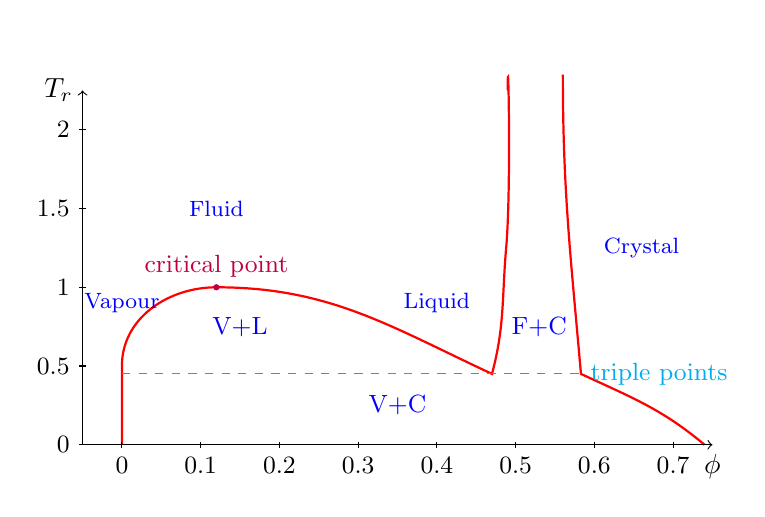
\begin{tikzpicture}
            \draw[thick,red] (0.5,0) to[out=90,in=270] (0.5,1) to[out=90,in=180] (1.7,2) to[out=0,in=155] (5.2,0.9) to[out=75,in=265] (5.38,2.5) to[out=85,in=90] (5.4,4.5);
            \draw[thick,red] (6.1,4.7) to[out=270,in=95](6.33,0.9) to[out=335,in=140] (7.9,0);
            \draw[->] (0,0)--(8,0)node[below]{\(\phi\)};
            \draw[->] (0,0)--(0,4.5)node[left]{\(T_r\)};
            \foreach \x in {0,0.1,0.2,0.3,0.4,0.5,0.6,0.7}{
                \draw (10*\x+0.5,0.04)--(10*\x+0.5,-0.04)node[below]{\small \(\x\)};
            }
            \foreach \y in {0,0.5,1,1.5,2}{
                \draw (0.04,2*\y)--(-0.04,2*\y)node[left]{\small \(\y\)};
            }
            \draw[cyan,dashed] (0.5,0.9)--(6.33,0.9) node[right]{\small triple points};
            \node[blue] at (4,0.5) {\small V+C};
            \node[blue] at (2,1.5) {\small V+L};
            \node[blue] at (5.8,1.5) {\small F+C};
            \node[blue] at (0.5,1.8) {\footnotesize Vapour};
            \node[blue] at (4.5,1.8) {\footnotesize Liquid};
            \node[blue] at (1.7,3) {\footnotesize Fluid};
            \node[blue] at (7.1,2.5) {\footnotesize Crystal};
            \fill[purple] (1.7,2) circle (0.04) node[above]{\small critical point};
        \end{tikzpicture}
        \caption{Longuet--Higgins--Widom-style phase diagram for the `exact' van der Waals model. This phase diagram was computed by using the hard-sphere system as a reference system and adding a weak, long-ranged attractive interaction.}
    \end{figure}

    \subsubsection{The Critical Point}
    Let's now return to discuss what happened at the critical point. Mathematically, a critical point corresponds to where
    \begin{equation}
        \pdv{P}{V}=\pdv[2]{P}{V}=0\,.
    \end{equation}
    Having an expression of the pressure, we can of course solve for this condition by brute force, but there is a slightly more elegant way to find the critical point. We will again use the notation \(v=V/N\) to denote the volume per particle to reduce some notational cluttering. We rearrange the van der Waals equation to get a cubic
    \begin{equation}
        Pv^3-(Pb+k_B T)v^2+av-ab=0\,.
    \end{equation}
    For \(T<T_c\), the equation has three real roots, while for \(T>T_c\), there is just one. This means that precisely at the \(T=T_c\), the three roots must therefore coincide before two of them move off onto the complex plane. This means that at the critical point, the curve can be rewritten as
    \begin{equation}
        P_c(v-v_c)^3=0\,.
    \end{equation}
    By comparing the coefficients, we get
    \begin{equation}
        k_B T_c=\frac{8a}{27b}\quad,\quad v_c=3b\quad,\quad P_c=\frac{a}{27b^2}\,.
    \end{equation}

    \subsubsection*{The Law of Corresponding States Revisited}
    This time, we can express the temperature, pressure and volume in reduced quantities relative to the critical values
    \begin{equation}
        T_r\coloneqq\frac{T}{T_c}\quad,\quad v_r\coloneqq\frac{v}{v_c}\quad,\quad p_r\coloneqq\frac{P}{P_c}
    \end{equation}
    and rewrite the van der Waals equation of state into a form universal to all gases
    \begin{equation}
        P_r=\frac{8T_r}{3v_r-1}-\frac{3}{v_r^2}\,.
    \end{equation}
    This again illustrates the law of corresponding states. Moreover, since the three critical quantities \(T_c\), \(P_c\) and \(V_c\) are written in just two variables \(a\) and \(b\), we can construct a combination of them which is independent of \(a\) and \(b\) and therefore should be the same for all gases. This is the universal compressibility ratio
    \begin{equation}
        \frac{P_c v_c}{k_B T_c}=\frac{3}{8}\,.
    \end{equation}
    Comparing to real gases, for which this value ranges from \(0.28\) to \(0.30\), our proposed value is a little high. We shouldn't be too discouraged by this; after all, we knew from the beginning that the van der Waals equation is unlikely to be accurate in the liquid regime where the particle number density is high.

    \subsubsection*{Critical Exponents}
    We now turn to ask a different question. How do various quantities change as we approach the critical point?

    First, we can ask what happens to the difference in (inverse) densities \(v_{\text{gas}}-v_{\text{liquid}}\) as we approach the critical point along the coexistence curve. For \(T<T_c\), or equivalently \(T_r<1\), the reduced van der Waals equation has two stable solutions
    \begin{equation}
        P_r=\frac{8T_r}{3v_{r,\text{gas}}-1}-\frac{3}{v_{r,\text{gas}}^2}=\frac{8T_r}{3v_{r,\text{liquid}}-1}-\frac{3}{v_{r,\text{liquid}}^2}\,.
    \end{equation}
    Solving this for \(T_r\), we get
    \begin{equation}
        T_r=\frac{(3v_{r,\text{liquid}}-1)(3v_{r,\text{gas}}-1)(v_{r,\text{liquid}}+v_{r,\text{gas}})}{8v_{r,\text{liquid}}^2 v_{r,\text{gas}}^2}\,.
    \end{equation}
    Notice that as we approach the critical point, \(v_{r,\text{liquid}},v_{r,\text{gas}}\to 1\) and the equation above tells us that \(T_r\to 1\) as expected. We can see exactly how we approach \(T_r=1\) by expanding the right-hand side for small \(\epsilon=v_{r,\text{gas}}-v_{r,\text{liquid}}\). To do this quickly, it's best to notice that the equation is symmetric in \(v_{r,\text{gas}}\) and \(v_{r,\text{liquid}}\), so close to the critical point we can write \(v_{r,\text{gas}}=1+\epsilon/2\) and \(v_{r,\text{liquid}}=1-\epsilon/2\). Substituting this into the equation above and keeping just the leading order term, we find
    \begin{equation}
        T_r\approx 1-\frac{1}{16}(v_{r,\text{gas}}-v_{r,\text{liquid}})^2\,,
    \end{equation}
    or rearranging, as we approach \(T_c\),
    \begin{equation}
        v_{\text{gas}}-v_{\text{liquid}}\sim(T_c-T)^{1/2}\,.
    \end{equation}
    This answers our first question.

    Our second question is: how does the volume change with pressure as we move along the critical isotherm? It turns out that we can answer this question without doing any work. We know that at the critical point, \(\partial P/\partial v=\partial^2 P/\partial v^2=0\), so a Taylor expansion around the critical point must start with the cubic term,
    \begin{equation}\label{pressure_critical_exponent}
        P-P_c\sim(v-v_c)^3\,.
    \end{equation}
    This answers our second question.

    Our final question concerns the compressibility, defined as
    \begin{equation}
        \kappa=-\frac{1}{v}\left(\pdv{v}{P}\right)_T\,.
    \end{equation}
    We want to understand how changes as we approach \(T\to T_c\) from above. We already know that at the critical point \(\partial P/\partial v=0\). So expanding for temperatures close to \(T_c\), we expect
    \begin{equation}
        \left(\pdv{P}{v}\right)_{T=T_c}=-a(T-T_c)+\dots
    \end{equation}
    This tells us the compressibility should diverge at the critical point, scaling as
    \begin{equation}\label{kappa_critical_exponent}
        \kappa\sim (T-T_c)^{-1}\,.
    \end{equation}

    We now have three answers to three questions:
    \begin{align}
        v_{\text{gas}}-v_{\text{liquid}}&\sim(T_c-T)^{\beta} & \beta&=\frac{1}{2} \\
        P-P_c&\sim(v-v_c)^\delta & \delta&=3 \\
        \kappa&\sim(T-T_c)^{-\gamma} & \gamma&=1\,.
    \end{align}
    Do they agree with experiment? Remember that we're not sure that we can trust the van der Waals equation at the critical point so we should be nervous. However, there is also reason for some confidence. Notice, in particular, that when computing (\ref{pressure_critical_exponent}) and (\ref{kappa_critical_exponent}), we didn't actually need any details of the van der Waals equation. We simply needed to assume the existence of the critical point and an analytic Taylor expansion of various quantities in the neighbourhood. Given that the answers follow from such general grounds, one may hope that they provide the correct answers for a gas in the neighbourhood of the critical point even though we know that the approximations that went into the van der Waals equation aren't valid there. Fortunately, that isn't the case: the physics is much more interesting than that!

    The experimental results for a gas in the neighbourhood of the critical point do share one feature in common with the discussion above: they are completely independent of the atomic make-up of the gas --- again illustrating the law of corresponding states. However, the scaling that we computed using the van der Waals equation is not fully accurate. The correct results are as follows:
    \begin{align}
        v_{\text{gas}}-v_{\text{liquid}}&\sim(T_c-T)^{\beta} & \beta&\approx 0.32 \\
        P-P_c&\sim(v-v_c)^\delta & \delta&\approx4.8 \\
        \kappa&\sim(T-T_c)^{-\gamma} & \gamma&\approx 1.2\,.
    \end{align}
    The quantities \(\beta\), \(\gamma\) and \(\delta\) are examples of \textit{critical exponents}. The van der Waals equation provides only a crude first approximation to the critical exponents.

    \subsubsection*{Fluctuations}
    We see that the van der Waals equation didn't do too badly in capturing the dynamics of an interacting gas. It gets the qualitative behaviour right, but fails on precise quantitative tests. So what went wrong? We mentioned during the derivation of the van der Waals equation that we made certain approximations that are valid only at low density. So perhaps it is not surprising that it fails to get the numbers right near the critical point where \(v=3b\). But there's actually a deeper reason that the van der Waals equation fails: fluctuations.

    This is simplest to see in the grand canonical ensemble. You will show in one of the exercises that \(\Delta N/N\sim 1/\sqrt{N}\), which essentially allows us to work in a grand canonical ensemble even when we have a fixed particle number under normal conditions. In the context of the liquid-gas transition, fluctuating particle number is the same thing as fluctuating density \(\rho=N/V\). You will also show in one of the exercises that
    \begin{equation}
        \frac{\Delta N^2}{N}=-\frac{1}{\beta V}\left(\pdv{\eval{N}}{V}\right)_{p,T}\left(\pdv{V}{p}\right)_{N,T}\,.
    \end{equation}
    This relates the fluctuations in the particle number to the compressibility, which is diverging at the critical point. This means that there are large fluctuations in the density of the fluid at this point. The result is that any simple equation of state, like the van der Waals equation, which works only with the average volume, pressure and density will miss this key aspect of the physics.

    Understanding how to correctly account for these fluctuations is the subject of critical phenomena, which is unfortunately a far deeper subject. It has close links with the renormalization group and conformal field theory which also arise in fancy places like particle physics and string theory. We will briefly account for this in the appendix \cref{Chap:Landau_Ginzburg} using Landau--Ginzburg theory.

    \subsubsection*{Universality}
    Something magical happens if you try to compute the critical exponents of the Ising model under our mean field treatment using the method analogous to above. They are given by
    \begin{align}
        m_0&\sim(T_c-T)^{\beta} & \beta&=\frac{1}{2} \\
        B&\sim m^\delta & \delta&=3 \\
        \chi&\sim(T-T_c)^{-\gamma} & \gamma&= 1\,,
    \end{align}
    where \(m=\eval{s}\) is the mean magnetisation, \(m_0\) is the mean magnetisation at \(B=0\) and \(\kappa\) is the magnetic susceptibility defined as
    \begin{equation}
        \chi=N\left(\pdv{m}{B}\right)_T\,.
    \end{equation}

    These critical exponents are exactly the ones that we have calculated for the van der Waals equation of state!

    We saw that the mean field approach to the Ising model gave the same critical exponents as the van der Waals equation. They are both wrong, and they are both wrong in the same, complicated, way with regard to the same true answer! Why on earth would a system of spins on a lattice have anything to do with the phase transition between a liquid and gas? It is as if all memory of the microscopic physics --- the type of particles, the nature of the interactions --- has been lost at the critical point. And that's exactly what happens.

    What we're seeing here is evidence for \textit{universality}. There is a single theory which describes the physics at the critical point of the liquid gas transition, the 3D Ising model and many other systems. This is a theoretician's dream! We spend a great deal of time trying to throw away the messy details of a system to focus on the elegant essentials. But, at a critical point, Nature does this for us! Although critical points in two dimensions are well understood, there is still much that we don't know about critical points in three dimensions.

    \subsection{Widom's Particle Insertion Method}
    We all have an intuitive idea of what most thermodynamic variables are, like temperature, pressure, volume \textit{etc.}, but the chemical potential \(\mu\) still seems a little bit mysterious. Here, we will introduce an idea proposed by Benjamin Widom, which would help us to understand chemical potential in an intuitive way, and calculate it easily.

    Consider a one-component system of \(N\) particles, with Helmholtz energy \(A=-k_B T\ln Q(N,V,T)\). Then for sufficiently large \(N\), we can effectively treat the number of particles as a continuum. The chemical potential is given by
    \begin{align}\label{insertion_potential}
        \mu=\left(\pdv{A}{N}\right)_{V,T}&= -k_B T\lim_{\Delta N\to 0}\frac{\ln Q(N+\Delta N,V,T)-\ln Q(N,V,T)}{\Delta N}\notag \\
        &\approx -k_B T\ln\left(\frac{Q(N+1,V,T)}{Q(N,V,T)}\right)\,.
    \end{align}
    \(\Delta N=1\) is the smallest variation we can do. This should hold when \(N\) is large and we can effectively treat \(\Delta N=1\) as an ``infinitesimal'' change.

    For an ideal gas, \(Q(N,V,T)=V^N/\Lambda^{3N}N!\), and so using (\ref{insertion_potential}), the chemical potential is
    \begin{equation}
        \mu^{\text{id}}=-k_B T\ln\left(\frac{V}{\Lambda^3(N+1)}\right)\,.
    \end{equation}
    In the \(N\to\infty\) limit, this agrees with a perhaps more familiar form of the chemical potential of an ideal gas
    \begin{equation}
        \mu^{\text{id}}=k_B T\ln(\Lambda^3\rho)\,,
    \end{equation}
    where \(\rho=N/V\) is the particle number density. Then for a non-ideal gas system, we may define the \textit{excess chemical potential} as
    \begin{align}
        \mu^{\text{ex}}(N/V,T)&\coloneqq\mu(N/V,T)-\mu^{\text{id}}(N/V,T)\notag\\
        &=-k_B T\ln\left(\frac{\int\prod_{j=1}^{N+1}\dd[3]{\vb{r}_j}\exp[-\beta U(\{\vb{r}_i\}_{i=1}^{N+1})]}{V\int\prod_{j=1}^{N}\dd[3]{\vb{r}_j}\exp[-\beta U(\{\vb{r}_i\}_{i=1}^{N})]}\right)\,.
    \end{align}
    We separate the potential energy of the \(N+1\)-particle system as a sum of the \(N\)-particle system and the interaction energy of the \(N+1^{\text{th}}\) particle with the rest of the system, so that \(U(\{\vb{r}_i\}_{i=1}^{N+1})=U(\{\vb{r}_i\}_{i=1}^{N})+\Delta U_{N,N+1}\). We can then rewrite
    \begin{align}
        \mu^{\text{ex}}(N/V,T)&=-k_B T\ln\left(\frac{\int\dd[3]{\vb{r}_{N+1}}\int\prod_{i=1}^{N}\dd[3]{\vb{r}_i}\exp[-\beta U(\{\vb{r}_i\}_{i=1}^{N})]\exp[-\beta\Delta U_{N,N+1}]}{V\int\prod_{j=1}^{N}\dd[3]{\vb{r}_j}\exp[-\beta U(\{\vb{r}_i\}_{i=1}^{N})]}\right)\notag\\
        &=-k_B T\ln\left(\frac{1}{V}\int\dd[3]{\vb{r}_{N+1}}\eval{\exp(-\beta\Delta U_{N,N+1})}_N\right)\,.
    \end{align}
    Here \(\eval{-}_N\) denote the canonical ensemble average over the configuration space of the \(N\)-particles. In other words, the excess chemical potential is related to the average of \(\eval{\exp(-\beta\Delta U_{N,N+1})}_N\) over all possible positions of the particle \(N+1\). In a translationally invariant system, such as a liquid or a gas, this quantity should not depend \(\vb{r}_{N+1}\), so we may write
    \begin{equation}\label{Widom_formula}
        \mu^{\text{ex}}(N/V,T)=-k_B T\ln\eval{\exp(-\beta\Delta U_{N,N+1})}_N\,.
    \end{equation}
    This is often known as the particle insertion method because it relates the excess chemical potential to the average of the Boltzmann factor \(\exp(-\beta\Delta U_{N,N+1})\) associated with the random insertion of an additional particle in the system where \(N\) particles are already present.

    \subsubsection{Excess Chemical Potential of a Hard-Sphere Gas}
    As an example, let's calculate the excess chemical potential of a hard-sphere gas system. A trial particle is inserted into the system --- it has a probability \(P\) to not overlap with the already-existing \(N\) particles, and probability \(1-P\) to overlap with some of the particles. By the definition of a hard sphere potential, if there is no overlapping of particles, \(\Delta U_{N,N+1}=0\) so \(\exp(-\beta \Delta U_{N,N+1})=1\); if the particles overlap, \(\Delta U_{N,N+1}=\infty\) so \(\exp(-\beta \Delta U_{N,N+1})=0\). Hence we have the average
    \begin{equation}
        \eval{\exp(-\beta\Delta U_{N,N+1})}=P\times 1+(1-P)\times 0=P\,.
    \end{equation}
    The excess chemical potential is then
    \begin{equation}
        \mu^{\text{ex}}=-k_B T\ln P\,.
    \end{equation}

    \begin{figure}
        \centering
        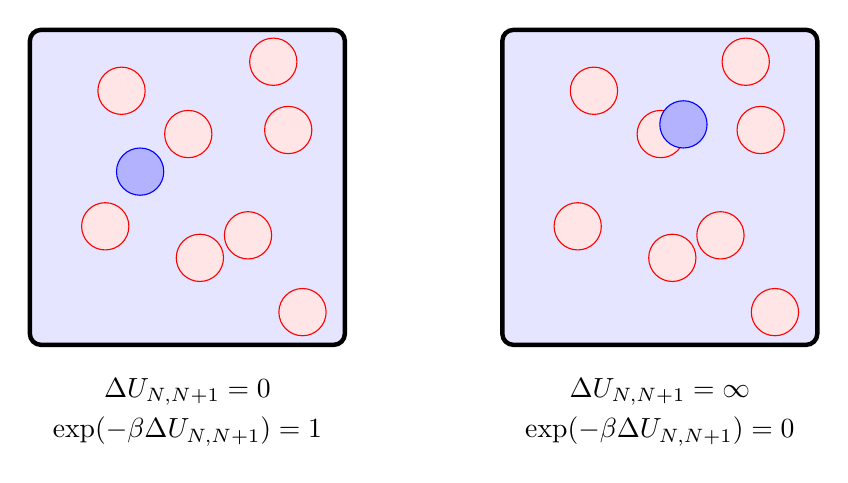
\begin{tikzpicture}
            \draw[ultra thick, rounded corners, fill=blue!10] (-2,-2) rectangle (2,2);
            \node at (0,-2.6){\(\Delta U_{N,N+1}=0\)};
            \node at (0,-3.1){\(\exp(-\beta\Delta U_{N,N+1})=1\)};
            \pgfmathsetseed{2}
            \foreach \i in {1,...,8}{
                \draw[red,fill=red!10] (1.6*rand,1.6*rand) circle (0.3);
            }
            \draw[blue,fill=blue!30] (-0.6,0.2) circle (0.3);

            \begin{scope}[shift={(6,0)}]
                \draw[ultra thick, rounded corners, fill=blue!10] (-2,-2) rectangle (2,2);
                \node at (0,-2.6){\(\Delta U_{N,N+1}=\infty\)};
                \node at (0,-3.1){\(\exp(-\beta\Delta U_{N,N+1})=0\)};
                \pgfmathsetseed{2}
                \foreach \i in {1,...,8}{
                    \draw[red,fill=red!10] (1.6*rand,1.6*rand) circle (0.3);
                }
                \draw[blue,fill=blue!30] (0.3,0.8) circle (0.3);
            \end{scope}
        \end{tikzpicture}
        \caption{A sample configuration of a hard sphere system.}

    \end{figure}

    \subsection{Virial Expansion for Classical Imperfect Gases}
    In the limit of dilute gas, the mean distance between the nearest-neighbour atoms greatly exceeds the range of the interatomic potential \(\phi(r)\). Under these conditions, the particles do not interact with each other except during very rare binary collisions, so we can treat them as ideal:
    \begin{equation}\label{ideal_compressibility}
        Z\coloneqq\frac{PV}{Nk_B T}=1
    \end{equation}
    when \(\rho^*=(N\sigma^3/V)\ll 1\). The probability of finding two atoms within a volume of the order of the atomic volume \(\sigma^3\) is of the order of \((\rho^*)^2\), and hence we expect deviation from ideal gas compressibility (\ref{ideal_compressibility}) as \(\rho^*\) increases. It therefore seems that we can express the compressibility factor of a non-ideal gas as a power series in the particle number density
    \begin{equation}
        Z\coloneqq\frac{P}{\rho k_B T}=1+B_2(T)\rho+B_3(T)\rho^2+\dots
    \end{equation}
    This is known as the \textit{virial expansion} of the compressibility factor, and the coefficients \(B_n(T)\) are known as the \textit{\(n^{\textit{th}}\) virial coefficient}.\footnote{Technically, this expansion is only valid if the interatomic potential decays sufficiently quickly. We will show this in appendix \cref{Chap:Cluster_Expansion}.}

    There is a traditional way in statistical mechanics to calculate these virial coefficients known as the \textit{cluster expansion}. This method is a bit mathematically challenging, and it gets more and more complicated when calculating higher orders of virial coefficients --- but it is a really elegant method, and it has important implications in some other related fields like perturbation theory or even quantum field theory. It is a shame not to mention it, so I put it in the appendix \cref{Chap:Cluster_Expansion}. However, Widom's particle insertion method provides us with an alternative easier way to calculate the second virial coefficient.\footnote{This method will encounter a whole lot of complications when we try to calculate higher virial coefficients, such as overlap of interaction zones \textit{etc.} If we are interested in them, the systematic cluster expansion is a much better choice.}

    First, we want to get an expression for \(\mu^{\text{ex}}\). From the Gibbs--Duhem relation \(V\d{P}=N\d{\mu}\), we get
    \begin{equation}\label{rho_Gibbs_Duhem}
        \pdv{P}{\rho}=\rho\pdv{\mu}{\rho}\,.
    \end{equation}
    As \(\mu^{\text{id}}=k_B T\ln(\rho\Lambda^3)\),
    \begin{equation}\label{ideal_gas_potential_diff}
        \frac{\rho}{k_B T}\pdv{\mu^{\text{id}}}{\rho}=1\,.
    \end{equation}
    If we differentiate the virial expansion with respect to \(\rho\), we get
    \begin{equation}
        \frac{1}{k_B T}\pdv{P}{\rho}=1+2B_2(T)\rho+3B_3(T)\rho^2+\dots
    \end{equation}
    From (\ref{rho_Gibbs_Duhem}), we can rewrite
    \begin{align}
        \frac{\rho}{k_B T}\pdv{\mu}{\rho}&=1+2B_2(T)\rho+3B_3(T)\rho^2+\dots\notag\\
        &=\frac{\rho}{k_B T}\pdv{\mu^{\text{id}}}{\rho}+2B_2(T)\rho+3B_3(T)\rho^2+\dots
    \end{align}
    where we observed that 1 corresponds to the derivative of the ideal gas chemical potential (\ref{ideal_gas_potential_diff}), so we can naturally relate the rest of the virial expansion with the derivative of the excess chemical potential
    \begin{equation}
        \frac{\rho}{k_B T}\pdv{\mu^{\text{ex}}}{\rho}=2B_2(T)\rho+3B_3(T)\rho^2+\dots
    \end{equation}
    Dividing this equation by \(\rho\) and integrating from 0 to \(\rho\), we obtain
    \begin{equation}
        \mu^{\text{ex}}=k_B T\sum_{n=2}^{\infty}\frac{n}{n-1}B_n(T)\rho^{n-1}=k_B T[2B_2\rho+\dots]\,.
    \end{equation}
    We can work out the expansion of the excess chemical potential to obtain the second virial coefficient.

    We then use Widom method (\ref{Widom_formula}) to work out \(\mu^{\text{ex}}\). In the regime of extremely dilute gas (\(\rho\to 0\)), we may assume an inserted particle will either have significant interaction with only one of the already-present \(N\) particles, or it will interact significantly with none of them, where we assumed that the interaction between particles will be negligible beyond some finite distance \(R_{\text{max}}\). This corresponds to a particle number density \(\rho\ll R_{\text{max}}^{-3}\), and our end result should be independent of \(R_{\text{max}}\). We may also assume that the interaction volumes \(v_{\text{int}}=\frac{4}{3}\pi R_{\text{max}}^3\) of the particles do not overlap. Then the total interaction volume of the \(N\) particles is
    \begin{equation}
        V_{\text{int}}=Nv_{\text{int}}=\frac{4}{3}N\pi R_{\text{max}}^3\,.
    \end{equation}

    \begin{figure}
        \centering
        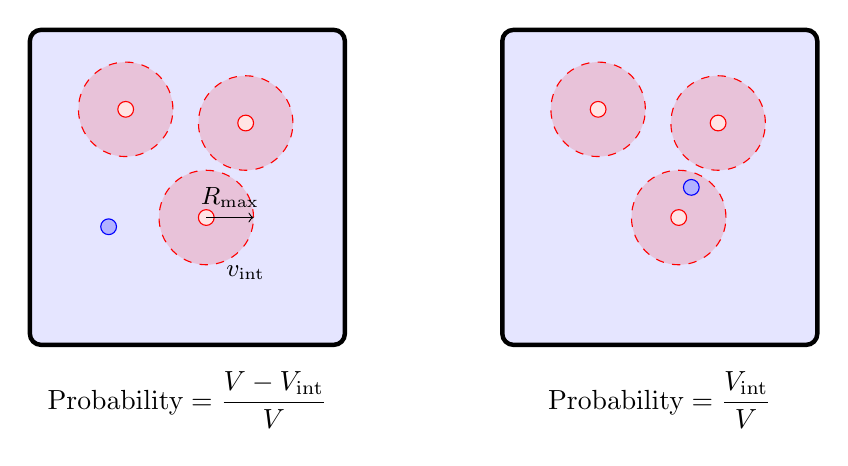
\begin{tikzpicture}
            \draw[ultra thick, rounded corners, fill=blue!10] (-2,-2) rectangle (2,2);
            \node at (0,-2.7){\(\displaystyle\text{Probability}=\frac{V-V_{\text{int}}}{V}\)};
            \pgfmathsetseed{8}
            \foreach \i in {1,2,3}{
                \tikzmath{
                    \x = 1.3 * rand;
                    \y = 1.3 * rand;
                }
                \draw[red,dashed,fill=red,fill opacity = 0.15] (\x,\y) circle (0.6);
                \draw[red,fill=red!10] (\x,\y) circle (0.1);
                \ifthenelse{\i = 3}{
                    \draw[->] (\x,\y)--node[above]{\small\(R_{\text{max}}\)}(\x + 0.6,\y);
                    \node at (\x+0.5,\y-0.7) {\small \(v_{\text{int}}\)};
                }{}
            }
            
            \draw[blue,fill=blue!30] (-1,-0.5) circle (0.1);

            \begin{scope}[shift={(6,0)}]
                \draw[ultra thick, rounded corners, fill=blue!10] (-2,-2) rectangle (2,2);
                \node at (0,-2.7){\(\displaystyle\text{Probability}=\frac{V_{\text{int}}}{V}\)};
                \pgfmathsetseed{8}
                \foreach \i in {1,2,3}{
                    \tikzmath{
                        \x = 1.3 * rand;
                        \y = 1.3 * rand;
                    }
                    \draw[red,dashed,fill=red,fill opacity = 0.15] (\x,\y) circle (0.6);
                    \draw[red,fill=red!10] (\x,\y) circle (0.1);
                }
                \draw[blue,fill=blue!30] (0.4,0) circle (0.1);
            \end{scope}
        \end{tikzpicture}
        \caption{Widom insertion method to determine the excess chemical potential of a dilute non-ideal gas system.}
    \end{figure}

    Now, if we insert a particle randomly, it has probability \((V-V_{\text{int}})/V\) to not fall into the interaction zone with any of the other particles, giving \(\Delta U=0\). With a probability \(V_{\text{int}}/V\), the insertion will happen in one of the interaction zones, and the average value of \(\exp(-\beta \Delta U)\) is
    \begin{equation}
        \frac{1}{v_{\text{int}}}\int_{v_{\text{int}}}\dd[3]{\vb{r}}\exp[-\beta\phi(\vb{r})]\,.
    \end{equation}
    Therefore, we have the average
    \begin{align}
        \eval{\exp(-\beta\Delta U_{N,N+1})}_N&=\left(\frac{V-V_{\text{int}}}{V}\right)+\left(\frac{V_{\text{int}}}{V}\right)\times\frac{1}{v_{\text{int}}}\int_{v_{\text{int}}}\dd[3]{\vb{r}}\exp[-\beta\phi(\vb{r})]\notag\\
        &=1+\rho\left(-v_{\text{int}}+\int_{v_{\text{int}}}\dd[3]{\vb{r}}\exp[-\beta\phi(\vb{r})]\right)\,.
    \end{align}
    Since \(v_{\text{int}}=\int_{v_{\text{int}}}\dd[3]{\vb{r}}\), we can write this as
    \begin{equation}
        \eval{\exp(-\beta\Delta U_{N,N+1})}_N=1+\rho\int_{v_{\text{int}}}\dd[3]{\vb{r}}[\exp(-\beta\phi(\vb{r}))-1]\,.
    \end{equation}
    By the Widom formula (\ref{Widom_formula}), we have
    \begin{equation}
        \mu^{\text{ex}}=-k_B T\ln\left(1+\rho\int_{v_{\text{int}}}\dd[3]{\vb{r}}[\exp(-\beta\phi(\vb{r}))-1]\right)\,.
    \end{equation}
    By construction, \(\phi(\vb{r})\approx 0\) outside the interaction zone, so we can change the limits of the integral to the whole space. Finally, as \(\rho v_{\text{int}}\ll 1\), we can use Taylor expansion \(\ln(1+x)\approx x\) to expand it to the first order
    \begin{equation}
        \mu^{\text{ex}}\approx k_B T\rho\int\dd[3]{\vb{r}}[1-\exp(-\beta\phi(\vb{r}))]\,.
    \end{equation}
    This is the term linear in \(\rho\) in the density expansion of \(\mu^{\text{ex}}\). Comparing with our expansion of \(\mu^{\text{ex}}\), we identify the second virial coefficient
    \begin{equation}
        B_2(T)=\frac{1}{2}\int\dd[3]{\vb{r}}[1-\exp(-\beta\phi(\vb{r}))]\,.
    \end{equation}
    If the potential is spherically symmetric, \(\phi(\vb{r})=\phi(r)\), we may write
    \begin{equation}
        B_2(T)=2\pi\int\dd{r}r^2[1-\exp(-\beta\phi(r))]\,.
    \end{equation}
    The quantity \(1-\exp(-\beta\phi(\vb{r}))\) occurring repeatedly in our expression is called the \textit{Mayer \(f\) function} and is usually denoted as \(f(r)\). It seems to just somehow randomly emerge in our derivation, but it actually has a significant importance in the canonical derivation of virial coefficients --- see appendix \cref{Chap:Cluster_Expansion}.

    \begin{figure}
        \centering
        \begin{tikzpicture}
            \node at (-1.5,4){(a)};
            \draw[->] (-0.3,0.5)--(4,0.5)node[below]{\(r/\sigma\)};
            \draw[->] (0,-0.5)--(0,3.5)node[left]{\(\phi(r)\)};
            \draw (1,0.4) node[below]{\(1\)}--(1,0.5);
            \draw[thick] (1,3.5)--(1,0.5)--(4,0.5);

            \node at (4.5,4){(b)};
            \draw[->] (5.7,0.5)--(10,0.5)node[below]{\(r/\sigma\)};
            \draw[->] (6,-0.5)--(6,3.5)node[left]{\(\phi(r)\)};
            \draw (7,0.9)--(7,1.1);
            \node at (6.8,0.2) {\(1\)};
            \node at (8.2,0.2) {\(\lambda\)};
            \draw (6,-0.1)--(5.9,-0.1)node[left]{\small\(-\epsilon\)};
            \draw[thick] (7,3.5)--(7,-0.1)--(8,-0.1)--(8,0.5)--(10,0.5);
        \end{tikzpicture}
        \caption{Two pair potentials: (a) Hard-sphere potential (b) Square-well potential.}
    \end{figure}

    Let's calculate \(B_2(T)\) for two simple interatomic potentials. First, let's consider the hard-sphere potential
    \begin{equation}
        \phi_{\text{HS}}(r)=\begin{cases}
            \infty & \text{if } r<\sigma \\
            0 & \text{if }r\ge \sigma\,,
        \end{cases}
    \end{equation}
    and so \(f(r)=-1\) if \(r<\sigma\) and \(f(r)=0\) otherwise. Thus
    \begin{equation}
        B_2^{\text{HS}}(T)=\frac{2\pi\sigma^3}{3}\,.
    \end{equation}
    It is a half of the excluded volume around a sphere. In this case, \(B_2\) is independent of temperature, and hence such a system is called \textit{athermal}. It reflects the fact that there is no energy scale in the hard-sphere potential --- no matter how high the temperature, the entropy never wins the infinite energy when particles overlap. The corresponding correction in \(Z\) (or equivalently \(P\)) from ideal gas law is positive, as the hard-sphere potential is purely repulsive.

    Next, consider the square-well potential
    \begin{equation}
        \phi_{\text{SW}}(r)=\begin{cases}
            \infty & \text{if }r<\sigma \\
            -\epsilon & \text{if }\sigma\le r<\lambda\sigma \\
            0 & \text{if }r\ge\lambda\sigma\,.
        \end{cases}
    \end{equation}
    Here, \(\epsilon\) parameterises the depth of the well and \(\lambda\) parameterises its width. In this case, 
    \begin{equation}
        B_2^{\text{SW}}(T)=\frac{2\pi\sigma^3}{3}\left[1-(\lambda^3-1)(\exp(\beta\epsilon)-1)\right]\,.
    \end{equation}
    This is plotted in the figure below. \(B_2(T)\) can be both positive and negative --- in low \(T\), \(B_2<0\) because attraction dominates, whilst at high \(T\), \(k_B T\gg \epsilon\) so the attractive part of the potential is unimportant, while the thermal energy still can't break the infinitely high potential barrier of the hard particle core, so the hard-sphere limit is recovered. The temperature at which \(B_2(T)=0\) is called the \textit{Boyle temperature}, because at this temperature, the system behaves very close to being ideal (at least to the first order in \(\rho\)).
    
    \begin{figure}
        \centering
        \begin{tikzpicture}
            \draw[->] (0,-3)--(0,1.5)node[left]{\(B_2^{\text{SW}}/B_2^{\text{HS}}\)};
            \draw[->] (0,0)--(5,0)node[above]{\(\beta\epsilon\)};
            \draw (0,1)--(-0.1,1)node[left]{\small\(1\)};
            \draw[thick, domain=0:5,samples=100, smooth, variable=\x] plot ({\x}, {2-2.72^(0.3*\x)});
        \end{tikzpicture}
        \caption{A plot of \(B_2(T)\) against \(\beta\epsilon\). The temperature at which \(B_2(T)=0\) is the Boyle temperature.}
    \end{figure}

    \subsection{Flory--Huggins Theory of Polymer Solutions}
    Let's consider polymers living on a lattice. Suppose we have a cubic lattice of \(M\) sites in total, and we have \(N\) monodisperse (of the same size) polymer molecules, each comprises \(r\) segments. Each lattice site can either be occupied by a single polymer segment, or it will be taken up by the solvent. The polymer chain is connected by covalent bonds, which we are never going to break in any cases, so we may safely ignore their contributions to the energy of our system --- it is just an additive constant. We further assume that neighbouring polymer segments that are not covalently bonded has an interaction energy \(\epsilon_{\text{PP}}\); neighbouring solvent molecules interact with energy \(\epsilon_{\text{SS}}\); neighbouring solvent-polymer segment pair interact with \(\epsilon_{\text{SP}}\).

    \begin{figure}
        \centering
        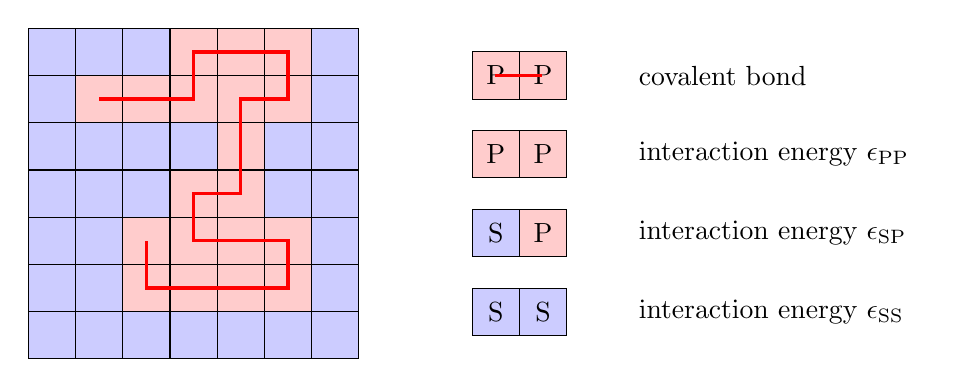
\begin{tikzpicture}
            \fill[blue!20] (0,0) rectangle (4.2,4.2);
            \fill[red!20] (0.6,3) rectangle (1.8,3.6);
            \fill[red!20] (1.8,3) rectangle (3.6,4.2);
            \fill[red!20] (2.4,1.8) rectangle (3,3);
            \fill[red!20] (1.8,1.8) rectangle (2.4,2.4);
            \fill[red!20] (1.2,0.6) rectangle (3.6,1.8);
            \foreach \x in {0,...,7}{
                \draw (0.6*\x,0)--(0.6*\x,4.2);
                \draw (0,0.6*\x)--(4.2,0.6*\x);
            }
            \draw[very thick, red] (0.9,3.3)--(2.1,3.3)--(2.1,3.9)--(3.3,3.9)--(3.3,3.3)--(2.7,3.3)--(2.7,2.1)--(2.1,2.1)--(2.1,1.5)--(3.3,1.5)--(3.3,0.9)--(1.5,0.9)--(1.5,1.5);

            \node at (5.5,2.1)[right]{\tikz{
                \draw (0,0) node[minimum height=0.6cm,minimum width=0.6cm,draw,fill=blue!20] {S};
                \draw (0.6,0) node[minimum height=0.6cm,minimum width=0.6cm,draw,fill=blue!20] {S};
                \node at (2,0)[right]{interaction energy \(\epsilon_{\text{SS}}\)};
                \draw (0,1) node[minimum height=0.6cm,minimum width=0.6cm,draw,fill=blue!20] {S};
                \draw (0.6,1) node[minimum height=0.6cm,minimum width=0.6cm,draw,fill=red!20] {P};
                \node at (2,1)[right]{interaction energy \(\epsilon_{\text{SP}}\)};
                \draw (0,2) node[minimum height=0.6cm,minimum width=0.6cm,draw,fill=red!20] {P};
                \draw (0.6,2) node[minimum height=0.6cm,minimum width=0.6cm,draw,fill=red!20] {P};
                \node at (2,2)[right]{interaction energy \(\epsilon_{\text{PP}}\)};
                \draw (0,3) node[minimum height=0.6cm,minimum width=0.6cm,draw,fill=red!20] {P};
                \draw (0.6,3) node[minimum height=0.6cm,minimum width=0.6cm,draw,fill=red!20] {P};
                \draw[red, very thick] (0.3,3)--(0.9,3);
                \node at (2,3)[right]{covalent bond};
            }};
        \end{tikzpicture}
    \end{figure}

    We will again use mean field approximation and calculate the excess chemical potential using Widom's insertion method. If we replace \(r\) solvent sites by a polymer chain of length \(r\), then
    \begin{equation}
        \mu^{\text{ex}}=-k_B T\ln\eval{\exp(-\beta\Delta U)}\,.
    \end{equation}

    First, let's calculate the probability that the inserted polymer does not overlap with the already-existing \(N\) polymer. If we denote the fractional occupation by
    \begin{equation}
        \eta=\frac{Nr}{M}\,,
    \end{equation}
    then the probability of the successful insertion of the first segment without overlapping is given by \(1-\eta\). We then encounter some problems. The insertion of successive segments in a polymer chain is correlated --- if the first segment is inserted near a polymer chain, then the probability of overlapping when inserting the second segment is very high, since the second segment must be in a neighbouring site of the first segment. On the other hand, if the first segment inserted is far from any other polymers, then the second segment has zero probability of overlapping. To make some progress, we will make a drastic simplification that the probabilities for the successful insertion of subsequent segments are uncorrelated, i.e. the inserted segments are not connected.\footnote{As you can tell, this is a horribly drastic assumption. If our model goes wrong compared with experiments, this is likely to be the main culprit (but rather surprisingly, our model actually agrees with the experiments astonishingly well!).} Then the probability that a single chain can be inserted without overlaps is \((1-\eta)^r\).

    Next, we compute the average energy change of a successful insertion. Again, to simplify our calculation, we have to assume that the inserted segments are decoupled. Moreover, we further assume that the existing polymers are also distributed randomly in the lattice sites. Therefore, for any particular inserted segment, the probability of any particular neighbour being occupied by an existing polymer segment is \(\eta\), and the probability of it being a solvent is \(1-\eta\). Therefore, the average change in energy of any nearest neighbour pair is
    \begin{align}
        \Delta\epsilon_{\text{nn}}&=\eta(\epsilon_{\text{{PP}}}-\epsilon_{\text{SP}})+(1-\eta)(\epsilon_{\text{SP}}-\epsilon_{\text{SS}})\notag\\
        &=\eta(\epsilon_{\text{PP}}+\epsilon_{\text{SS}}-2\epsilon_{\text{SP}})+(\epsilon_{\text{SP}}-\epsilon_{\text{SS}})\,.
    \end{align}
    If we denote
    \begin{align}
        \Delta\epsilon&\coloneqq\epsilon_{\text{SP}}-\frac{\epsilon_{\text{PP}}+\epsilon_{\text{SS}}}{2}\\
        \delta\epsilon&\coloneqq\epsilon_{\text{SP}}-\epsilon_{\text{SS}}\,,
    \end{align}
    then the average total change in energy of inserting a polymer of \(r\) segments is
    \begin{align}
        \Delta U&=rz\Delta\epsilon_{\text{nn}}\notag\\
        &=-2rz\eta\Delta\epsilon+rz\delta\epsilon\,,
    \end{align}
    where \(z\) is the average number of non-bonded nearest neighbours of a segment.

    Now we can estimate \(\mu^{\text{ex}}\) using Widom's formula, which gives
    \begin{equation}\label{Flory_Huggins_mu_ex}
        \mu^{\text{ex}}=rk_B T\ln(1-\eta)-2rz\eta\Delta\epsilon+rz\delta\epsilon\,.
    \end{equation}
    The ideal contribution to the chemical potential of \(N\) polymers is
    \begin{equation}
        \mu^{\text{id}}=k_B T\ln\frac{N}{M}=k_B T\ln\eta-k_B T\ln r\,.
    \end{equation}
    We add these two terms together and throw away all the constant terms independent of \(\eta\) (since they don't affect the phase behaviour), then the mean field chemical potential of the polymer solution is
    \begin{equation}
        \mu=k_B T\ln\eta-rk_B T\ln(1-\eta)-2rz\eta\Delta\epsilon+\text{const.}
    \end{equation}
    It is common to define the \textit{Flory--Huggins parameter} \(\chi\) by
    \begin{equation}
        \chi\coloneqq\frac{z\Delta\epsilon}{k_B T}\,,
    \end{equation}
    then we get
    \begin{equation}
        \mu=k_B T(\ln\eta-r\ln(1-\eta)-2r\chi\eta)\,,
    \end{equation}
    where we have omitted the constant term. This is the \textit{Flory--Huggins expression} for the chemical potential of a polymer solution.

    \subsubsection{Flory--Huggins Critical Point}
    It is experimentally observed that a polymer solution shows phase behaviour, where below a certain critical temperature, a polymer solution with some \(\eta\) values will separate into phases. Let's rationalise this behaviour using the chemical potential we calculated.

    \begin{figure}
        \centering
        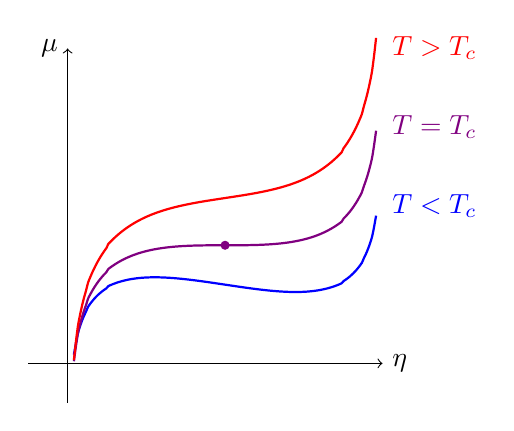
\begin{tikzpicture}
            \draw[->] (-0.5,0)--(4,0)node[right]{\(\eta\)};
            \draw[->] (0,-0.5)--(0,4)node[left]{\(\mu\)};
            \draw[thick, blue, domain=0.02:0.98,samples=150, smooth, variable=\x] plot ({4*\x}, {2.5+1.5*(0.4*ln(\x)-0.4*ln(1-\x)-2*\x)});
            \draw[thick, violet, domain=0.02:0.98,samples=150, smooth, variable=\x] plot ({4*\x}, {3.0+1.5*(0.5*ln(\x)-0.5*ln(1-\x)-2*\x)});
            \draw[thick, red, domain=0.02:0.98,samples=150, smooth, variable=\x] plot ({4*\x}, {3.6+1.5*(0.6*ln(\x)-0.6*ln(1-\x)-2*\x)});
            \node[red] at (4,4)[right]{\(T>T_c\)};
            \node[violet] at (4,3)[right]{\(T=T_c\)};
            \node[blue] at (4,2)[right]{\(T<T_c\)};
            \draw[violet,fill=violet] (2,1.5) circle (0.05);
        \end{tikzpicture}
        \caption{The Flory--Huggins chemical potential. Phase separation may occur when \(T<T_c\).}
    \end{figure}

    In order for a phase separation to occur, there must be two phases with different \(\eta\) values with the same chemical potential.\footnote{This is a necessary condition, but it is not sufficient --- the pressure must also be equal.} Therefore, a plot of \(\mu\) versus \(\eta\) must have a van der Waals loop (see \cref{vdW_loops}). As we increase the temperature, this loop will disappear when the maximum and the minimum of the \(\mu\)-\(\eta\) curve merge. Hence, to find the critical point, we only need to find the point where the equation
    \begin{align}
        \pdv{\beta\mu}{\eta}=\frac{1}{\eta}+\frac{r}{1-\eta}-2r\chi=0\notag\\
        \implies\quad 2r\chi\eta^2-2r\left(\chi-\frac{1}{2}+\frac{1}{2r}\right)\eta+1=0
    \end{align}
    has a double root.\footnote{When dealing with the van der Waals gas, we identified the critical point to be the point at which both the first and the second derivative of \(A\) with respect to \(V\) vanishes. One can show that this is equivalent to the condition here once we identify \(V\) with \(M\) as the lattice analogue, by showing
    \begin{equation}
        \left(\pdv{P}{M}\right)_{T}\propto\left(\pdv{\mu}{\eta}\right)_{T}
    \end{equation}
    using Gibbs--Duhem relation.} This happens at the point
    \begin{equation}
        \eta_{\text{crit}}=\frac{r\left(\chi_{\text{crit}}-\frac{1}{2}+\frac{1}{2r}\right)}{2r\chi_{\text{crit}}}
    \end{equation}
    when the discriminant vanishes:
    \begin{equation}
        r^2\left(\chi_{\text{crit}}-\frac{1}{2}+\frac{1}{2r}\right)^2=2r\chi_{\text{crit}}\,.
    \end{equation}
    Solving these conditions gives
    \begin{align}
        \chi_{\text{crit}}&=\frac{(1+\sqrt{r})^2}{2r}\\
        \eta_{\text{crit}}&=\frac{1}{1+\sqrt{r}}\,.
    \end{align}

    For \(r=1\), \(\eta_{\text{crit}}=0.5\) and \(\chi_{\text{crit}}=2\). The \(\mu\)-\(\eta\) diagram is symmetric, and this is in fact identical to the regular solution model which you will investigate in one of the exercises. As \(r\) increases, \(\eta_{\text{crit}}\) decreases as the \(\mu\)-\(\eta\) diagram becomes more and more asymmetric, and \(\chi_{\text{crit}}\) also decreases, so the critical temperature \(T_{\text{crit}}\) increases. In the limit of large polymers, \(\lim_{r\to\infty}\eta_{\text{crit}}=0\) and \(\lim_{r\to\infty}\chi_{\text{crit}}=\frac{1}{2}\).

    \begin{figure}
        \centering
        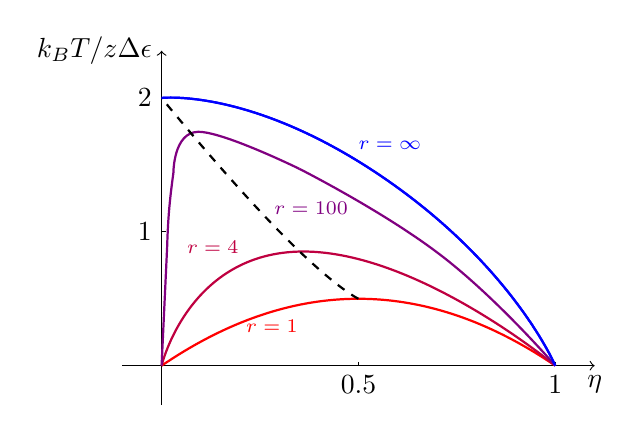
\begin{tikzpicture}
            \draw[->] (-0.5,0)--(5.5,0)node[below]{\(\eta\)};
            \draw[->] (0,-0.5)--(0,4)node[left]{\(k_B T/z\Delta\epsilon\)};
            \draw (5,0.05)--(5,0)node[below]{1};
            \draw (2.5,0.05)--(2.5,0)node[below]{0.5};
            \draw (0.05,1.7)--(0,1.7)node[left]{1};
            \draw (0.05,3.4)--(0,3.4)node[left]{2};
            \draw[thick, red, domain=0:1,samples=100, smooth, variable=\x] plot ({5*\x}, {3.4*\x*(1-\x)});
            \node[red] at (1.4,0.5) {\scriptsize\(r=1\)};
            \draw[thick, purple] plot [smooth, tension=1.05] coordinates { (0,0) (1.8,1.45) (5,0)};
            \node[purple] at (0.65,1.5) {\scriptsize\(r=4\)};
            \draw[thick, violet] (0,0)--(0.07,1.5) to[bend left=3] (0.15,2.45);
            \draw[thick, violet] plot [smooth, tension=0.7] coordinates { (0.15,2.45) (0.46,2.97) (1.75,2.5)};
            \draw[thick, violet] plot [smooth, tension=0.8] coordinates { (1.75,2.5) (3.55,1.4) (5,0)};
            \node[violet] at (1.9,2) {\scriptsize\(r=100\)};
            \draw[thick, blue] plot [smooth, tension=1.2] coordinates { (0,3.4) (2.8,2.4) (5,0)};
            \node[blue] at (2.9,2.8) {\scriptsize\(r=\infty\)};
            \draw[thick, blue] plot [smooth, tension=1.2] coordinates { (0,3.4) (2.8,2.4) (5,0)};
            \draw[thick, black, dashed] plot [smooth, tension=1] coordinates { (2.5,0.85) (1.5,1.7) (0,3.4)};
        \end{tikzpicture}
        \caption{The Flory--Huggins phase diagram.}
    \end{figure}

    What leads to the asymmetry of the phase diagram at non-unity \(r\)? We can investigate the energy and entropic change of mixing explicitly. Consider a fully mixed system with \(Nr\) polymer segments and \(M-Nr\) solvent particles. The potential energy contributed by each polymer segment is \(U_{\text{P}}=z\eta\epsilon_{\text{PP}}+z(1-\eta)\epsilon_{\text{SP}}\), and the energy contributed by each solvent particle is \(U_{\text{S}}=z\eta\epsilon_{\text{SP}}+z(1-\eta)\epsilon_{\text{SS}}\). If the polymers and the solvent are completely separated, then \(U_{\text{P}}^{\text{pre}}=z\epsilon_{\text{PP}}\) and \(U_{\text{S}}^{\text{pre}}=z\epsilon_{\text{SS}}\) respectively. Hence, the energy change of mixing is
    \begin{align}
        \Delta_{\text{mix}}U&=\frac{1}{2}[Nr(U_{\text{P}}-U_{\text{P}}^{\text{pre}})+(M-Nr)(U_{\text{S}}-U_{\text{S}}^{\text{pre}})]\notag\\
        &=Mz\Delta\epsilon\eta(1-\eta)=Mk_B T\chi\eta(1-\eta)\,.
    \end{align}
    This is symmetric in \(\eta\). If \(N_1\) particles of volume \(V_1\) and \(N_2\) particles of volume \(V_2\) are mixed, forming a mixture of volume \(V=V_1+V_2\), then the entropy change of mixing is
    \begin{equation}
        \Delta_{\text{mix}}S/k_B=N_1\ln\left(\frac{V}{V_1}\right)+N_2\ln\left(\frac{V}{V_2}\right)\,.
    \end{equation}
    In our case, we have \(N_1=V_1=M-Nr\) solvent particles and \(N_2=V_2=Nr\) polymer molecules. This gives
    \begin{align}
        \Delta_{\text{mix}}S/k_B&=(M-Nr)\ln\frac{M}{M-Nr}+N\ln\frac{M}{Nr}\notag\\
        &=-M\left[(1-\eta)\ln(1-\eta)+\frac{\eta}{r}\ln\eta\right]\,.
    \end{align} 
    We can see that this is asymmetric in \(\eta\).

    \subsubsection{Flory--Huggins Parameter}
    The Flory--Huggins parameter \(\chi\) actually has more physical meanings: it tells us whether a solvent is good or not for a given polymer. Recall the virial series for the excess chemical potential
    \begin{equation}
        \beta\mu^{\text{ex}}=2B_2\rho+\frac{3}{2}B_3\rho^2+\dots
    \end{equation}
    Using \(\rho=N/M\) and \(\eta=Nr/M\), we can rewrite the expansion in terms of \(\eta\)
    \begin{equation}
        \beta\mu^{\text{ex}}=\frac{2B_2}{r}\eta+\dots
    \end{equation}
    The virial expansion applies in the dilute regime, i.e. at small \(\eta\), and so we can use Taylor expansion \(\ln(1-x)\approx -x\) in the excess chemical potential (\ref{Flory_Huggins_mu_ex}) to write
    \begin{equation}
        \beta\mu^{\text{ex}}\approx r\eta+2r\eta\chi\,.
    \end{equation}
    Comparing the coefficients of the two expansions, we can get the second virial coefficient
    \begin{equation}
        B_2=r^2\left[\frac{1}{2}-\chi\right]\,.
    \end{equation}
    We find that when \(\chi=\frac{1}{2}\), \(B_2=0\) and the ideal behaviour is recovered (at least to the leading order). At this point, the energetic and entropic contributions cancel out exactly, and the polymer behaves like a freely joined chain (see later chapters). The conditions under which this is achieved are known as the \(\theta\) conditions (just like the Boyle temperature for non-ideal gas). By contrast, if the energetic penalty is smaller than the entropic gain, \(\chi<\frac{1}{2}\), the entropic term dominates and the second virial coefficient is positive. The polymer segments repel each other and maximise the mixing. This increases the osmotic pressure of the polymer solution, and we say that the solvent is a \textit{good solvent}. By contrast, if \(\chi>\frac{1}{2}\), then \(B_2<0\). The polymer segments attract each other, and the solvent is said to be a \textit{poor solvent}.

    \begin{figure}
        \centering
        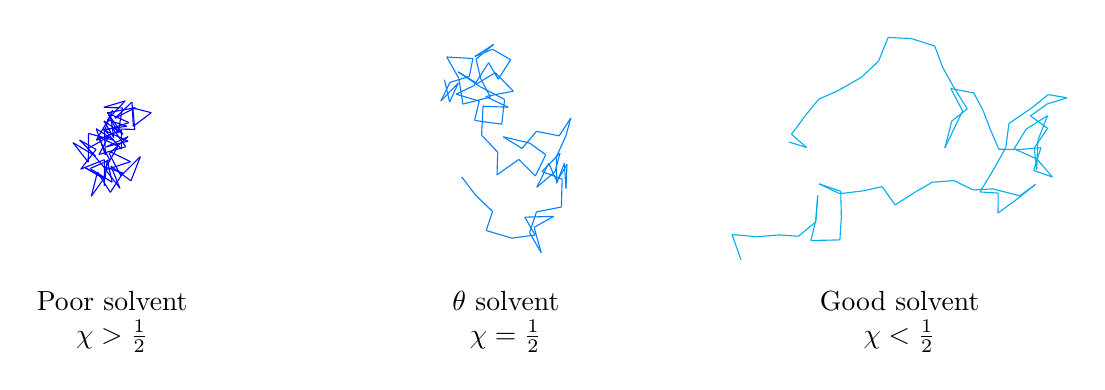
\begin{tikzpicture}
            \node at (-5,0){\tikz{\pgfmathsetseed{1}
            \coordinate (p) at (0,0);
            \pgfmathsetmacro{\a}{360*rnd}

            \foreach \i in {1,...,70}{
                \draw[blue] (p) -- ++({\a}: rand*0.07 + 0.3) coordinate (p);
                \pgfmathparse{mod(\a + 180 + 90*rand,360)}\xdef\a{\pgfmathresult}
            }}};

            \node at (0,0){\tikz{\pgfmathsetseed{12345}
            \coordinate (p) at (5,0);

            \foreach \i in {1,...,70}{
                \draw[blue!50!cyan] (p) -- ++(360*rand: rand*0.07 + 0.3) coordinate (p);
            }}};

            \node at (5,0){\tikz{\pgfmathsetseed{123456}
            \coordinate (p) at (10,0);
            \pgfmathsetmacro{\a}{360*rnd}

            \foreach \i in {1,...,70}{
                \draw[cyan] (p) -- ++({\a}: rand*0.07 + 0.3) coordinate (p);
                \pgfmathparse{mod(\a + 260*rand*rand,360)}\xdef\a{\pgfmathresult}
            }}};

            \node[align=center] at (-5,-2.2) {Poor solvent \\ \(\chi>\frac{1}{2}\)};
            \node[align=center] at (0,-2.2) {\(\theta\) solvent \\ \(\chi=\frac{1}{2}\)};
            \node[align=center] at (5,-2.2) {Good solvent \\ \(\chi<\frac{1}{2}\)};
        \end{tikzpicture}
        \caption{The effect of solvent quality on the behaviour of polymers in solution.}
    \end{figure}

    \subsection{Landau Theory of Phase Transitions}
    We have spent a long time investigating phase transitions for different systems case by case. But we have seen that the van der Waals equation and mean field Ising model gave the same wrong answers for the critical exponents with regard to the same true answer. This universality suggests that there should be a unified way to look at phase transitions. Such a method was developed by Lev Landau. It is worth stressing that the Landau approach to phase transitions often only gives qualitatively correct results. However, its advantage is that it is extremely straightforward and easy.

    \subsubsection{Order of Phase Transitions}
    Let's first introduce a classification of phase transitions. As we can see in previous sections, free energy plays an important role in phase transition, and hence a natural classification, introduced by Paul Ehrenfest, is based on how the free energy behaves at the critical point. The free energy itself of the two phases must be equal at the phase transition, so the free energy must be continuous at the critical point as a function of temperature or volume/pressure \textit{etc.} --- but its derivatives do not have to. If the first derivative of the free energy with respect to pressure/volume and temperature are discontinuous, then the transition is called a \textit{first order} phase transition. If the first derivatives are continuous, but the second ones are not, then the phase transition is called a \textit{second order} phase transition, and so on. There are rarely phase transitions above third order.\footnote{However, it should be pointed out that under modern theory of critical phenomena, this classification can no longer be strictly maintained --- but it is still a useful one.}

    The reason we are interested in this is that, a first order phase transition behaves very differently from a second order one. For example, if the first derivatives of the Gibbs free energy of some system are discontinuous, then there will be a volume change and a non-zero enthalpy of phase transition (which is the latent heat that you are familiar with)
    \begin{align}
        \left(\pdv{G_1}{P}\right)_T-\left(\pdv{G_2}{P}\right)_{T}&=V_1-V_2=\Delta_\text{trs}V\ne 0\\
        \left(\pdv{G_1}{T}\right)_{P}-\left(\pdv{G_2}{T}\right)_P&=-S_1+S_2=-\Delta_{\text{trs}}S=-\frac{\Delta_{\text{trs}}H}{T_{\text{trs}}}\ne 0\,.
    \end{align}
    Moreover, in a first order phase transition, a phase can remain metastable over a significant region. A famous example is the supercooling of water. In such metastable regions, the state of the system depends on its history. This phenomenon is known as \textit{hysteresis}. By contrast, in a continuous phase transition, the system smoothly passes to the new phase without needing to overcome any free energy barrier, making such transition very fast.

    Our aim is then to arrive at a unified theory to look at phase transitions and to determine whether a phase transition is first order or not in a simple way.
    \subsubsection{Free Energy Expansion and Order Parameter}
    What makes two phases different from each other? A plausible answer is symmetry. As Landau points out, a symmetry is either there or not there --- there isn't something like a partial symmetry. Just like a crystal is either cubic or it is not --- it cannot be `slightly cubic'. The symmetry of a system cannot change continuously.

    To quantify this, we introduce a concept called the \textit{order parameter}. It is some suitably chosen parameter in our system of interest that is zero in one of the phases and non-zero in another so that we hope when the phase transition occurs, the order parameter will jump from zero to a non-zero value. Sometimes it is obvious what to take as the order parameter; other times less so. For magnetic or electric systems, the order parameter is typically some form of magnetization (as for the Ising model) or the polarization. For the liquid-gas transition, the relevant order parameter is the difference in densities between the two phases, \(v_{\text{gas}}-v_{\text{liquid}}\). In something like a liquid crystal, as shown in \cref{liquid_crystal}, a suitable order parameter would be some sort of measurement of the average orientation of the molecules along some axis.

    \begin{figure}
        \centering
        \includegraphics[width=0.8\textwidth]{LC.png}
        \caption{A schematic diagram of the isotropic and nematic phases of a liquid crystal. The order parameter can be chosen to be \(M=\eval{3\cos^2\theta -1}/2\), which is 0 in the isotropic case, 1 if all particles are perfectly aligned along \(z\) axis, and \(-1/2\) if all particles are orthogonal to the \(z\) axis. Figure adapted from official course notes.}
        \label{liquid_crystal}
    \end{figure}

    Landau theory is based around the free energy, so the next thing we do is to write the free energy in terms of the order parameter. Let's be clear of what we are doing here. We have certainly worked out some expressions like this before. For example, in the Ising model, where the mean magnetisation \(m\) is the order parameter, we have worked out the free energy expression (\ref{Ising_MF_free_energy})
    \begin{equation}
        A=\frac{1}{2}NJzm^2-Nk_B T\ln[2\cosh(\beta Jzm)]\,.       
    \end{equation}
    But so far in this course, we've considered only systems in equilibrium. The free energy, like all other thermodynamic potentials, has only been defined on equilibrium states. Yet the equation above can be thought of as an expression for \(A\) as a function of \(m\), where \(m\) can be any number, including the non-equilibrium ones. Of course, what we should do is to substitute in the equilibrium value of \(m\) given by (\ref{Ising_equilibrium_condition}) to give the true equilibrium free energy with solid physical meaning, but it seems a shame to throw out \(A(m)\) when it is such a nice function. Surely we can put it to some use!
    
    The key in Landau theory is to treat the function \(A=A(N,V,T;m)\) seriously. This means that we are extending our viewpoint away from equilibrium states to a whole class of states which have a constant average value of \(m\). You could imagine some external magical power that holds \(m\) fixed. The free energy \(A(N,V,T;m)\) is then telling us the equilibrium properties in the presence of this magical power. Perhaps more convincing is what we do with the free energy in the absence of any magical constraint. We have seen that equilibrium is guaranteed if we sit at the minimum of \(A\). This means that what we want to do is to solve
    \begin{equation}
        \pdv{A}{m}=0\,,
    \end{equation}
    and find where \(A\) is the minimum. If this occurs at \(m=0\), then at this condition the disordered phase with zero value of order parameter is stable; if this occurs at non-zero value of \(m\), then the ordered phase is stable.

    However, finding an expression of the free energy \(A\) seems like a difficult thing to do. This is exactly what we have done in this whole chapter, spending a lot of efforts writing down the free energy of different system, which we have found is not an easy task even for simple models! Moreover, we promised that we will derive a general theory of phase transition, but the details of the free energy clearly depends on the physics of the system. How do we just write down the free energy in the general case? The trick is to assume that we can expand the free energy in an analytic power series in the order parameter. For this to be true, the order parameter must be small which is guaranteed if we are close to a critical point (since we assume that for \(T>T_c\) we have the disordered phase with \(m=0\)). This allows us to write
    \begin{equation}
        A(N,V,T,M)=A(N,V,T,0)+aM+bM^2+cM^3+dM^4+\dots
    \end{equation}
    Let's look at a couple of simple examples.
    \subsubsection{Second Order Phase Transitions}
    We first look at a system in which there is a symmetry in the order parameter by \(M\leftrightarrow -M\). An example of such a system is Ising model without external fields, where the order parameter is the magnetisation \(m\) --- a system with magnetisation \(+m\) is completely equivalent to a system with magnetisation \(-m\), so the free energy must be an even function of \(m\). We are investigating the phase transitions caused by changes in temperatures only, so for this kind of a system, we will write
    \begin{equation}
        A(T,M)=A(T,0)+b(T)M^2+d(T)M^4+f(T)M^6+\dots
    \end{equation}
    We will focus on the temperature regime where the quadratic coefficient changes its sign, since this is the lowest order term and should cause the greatest effect on the behaviour of \(A\) near \(M=0\). We will assume this sign change occurs at \(T=T_{\text{ch}}\) so that we can write, to the linear order, \(b(T)=\alpha(T-T_{\text{ch}})\). We will approximate higher coefficients to be constant near \(T=T_{\text{ch}}\). Let's see what happens if \(\alpha>0\) and \(d>0\), so that
    \begin{equation}
        A(T,M)\approx A(T,0)+\alpha(T-T_{\text{ch}})M^2+dM^4\,.
    \end{equation}
    A plot of \(A(T,M)\) at different \(T\) is shown in \cref{second_order_Landau}.

    \begin{figure}
        \centering
        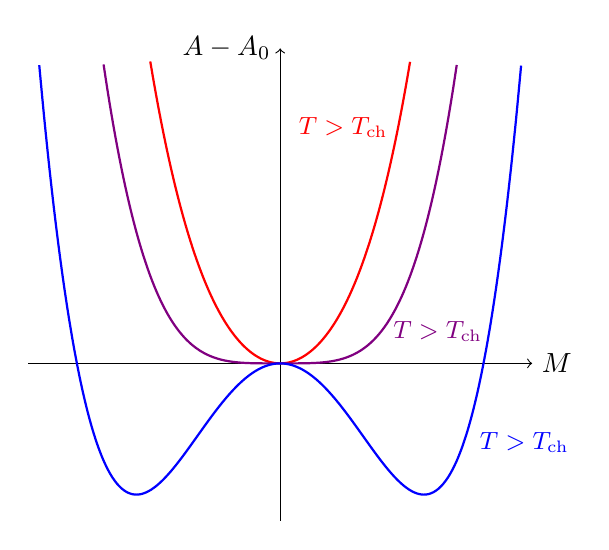
\begin{tikzpicture}
            \draw[->] (-3.2,0)--(3.2,0)node[right]{\(M\)};
            \draw[->] (0,-2)--(0,4)node[left]{\(A-A_0\)};
            \draw[thick, red, domain=-1.65:1.65,samples=100, smooth, variable=\x] plot ({\x}, {\x*\x+0.15*\x*\x*\x*\x});
            \draw[thick, violet, domain=-2.243:2.243,samples=100, smooth, variable=\x] plot ({\x}, {0.15*\x*\x*\x*\x});
            \draw[thick, blue, domain=-3.06:3.06,samples=100, smooth, variable=\x] plot ({\x}, {-\x*\x+0.15*\x*\x*\x*\x});
            \node[red] at (0.8,3){\small\(T>T_{\text{ch}}\)};
            \node[violet] at (2,0.4){\small\(T>T_{\text{ch}}\)};
            \node[blue] at (3.1,-1){\small\(T>T_{\text{ch}}\)};
        \end{tikzpicture}
        \caption{A sketch of the Landau free energy \(A\) as a function of the order parameter \(M\) for a system that is an even function of \(M\). The phase transition occurs at \(T=T_{\text{ch}}\), where the quadratic coefficient changes the sign if the quartic coefficient is assumed positive.}
        \label{second_order_Landau}
    \end{figure}

    It can be seen that, above \(T_{\text{ch}}\), the minimum of the free energy occurs at \(M=0\), so the disordered phase is more stable. Below \(T_{\text{ch}}\), the point \(M=0\) changes from being a minimum in free energy to a local maximum. Instead the minimum in the free energy is easily found to be
    \begin{equation}
        m=\pm\sqrt{\frac{\alpha(T_{\text{ch}}-T)}{2d}}\,.
    \end{equation}
    We can substitute this expression back into our free energy expansion, so that we know the free energy of the most stable state is
    \begin{equation}
        A_{\text{min}}=\begin{cases}
            A(T,0) & T\ge T_{\text{ch}} \\
            A(T,0)-\frac{\alpha^2(T-T_{\text{ch}}^2)}{4d} & T<T_{\text{ch}}\,.
        \end{cases}
    \end{equation}
    Assuming \(A(T,0)\) is a smooth function of \(T\), we can see that both the free energy and its first derivative are continuous at the phase transition. However, the second derivative, which is related to the heat capacity
    \begin{equation}
        C_V=-T\left(\pdv[2]{A}{T}\right)_{V}\,,
    \end{equation}
    is discontinuous. This is characteristic of a second-order phase transition.

    You will show in one of the exercises that the Ising model with no external field is exactly the situation depicted above by explicitly expanding the free energy.
    \subsubsection{First Order Phase Transition}
    If we relax the condition of the quartic coefficient \(d\) being positive, and instead assume that the \(M^6\) coefficient is positive, then we have the free energy expansion
    \begin{equation}
        A(T,M)\approx A(T,0)+\alpha(T-T_{\text{ch}})M^2+dM^4+fM^6
    \end{equation}
    with \(\alpha,f>0\) while \(d<0\). This leads to a more interesting tricritical point, which you will investigate in one of the exercises. Crucially, this time, the first derivative of the free energy is discontinuous at the critical temperature
    \begin{equation}
        T=T_{\text{ch}}+\frac{d^2}{4\alpha f}\,,
    \end{equation}
    so this results in a first order phase transition.

    Now, let's instead look at an important cases when \(A\) includes odd powers of \(M\).
    \begin{equation}
        A(T,M)=A(T,0)+\alpha(T-T_{\text{ch}})M^2+cM^3+dM^4+\dots
    \end{equation}
    We set \(\alpha,d>0\) while \(c<0\). A plot of \(A(M)\) at different \(T\) is shown in \cref{odd_Landau}.
    \begin{figure}
        \centering
        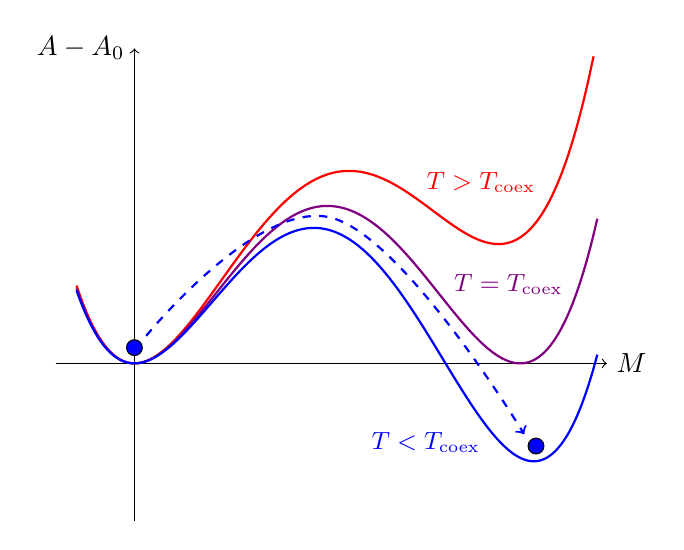
\begin{tikzpicture}
            \draw[->] (-1,0)--(6,0)node[right]{\(M\)};
            \draw[->] (0,-2)--(0,4)node[left]{\(A-A_0\)};
            \draw[thick, red, domain=-0.3:2.38,samples=100, smooth, variable=\x] plot ({2.45*\x}, {8.4*\x*\x-8*\x*\x*\x+2*\x*\x*\x*\x});
            \draw[thick, violet, domain=-0.3:2.4,samples=100, smooth, variable=\x] plot ({2.45*\x}, {8*\x*\x-8*\x*\x*\x+2*\x*\x*\x*\x});
            \draw[thick, blue, domain=-0.3:2.4,samples=100, smooth, variable=\x] plot ({2.45*\x}, {7.7*\x*\x-8*\x*\x*\x+2*\x*\x*\x*\x});
            \node[red] at (4.4,2.3){\small\(T>T_{\text{coex}}\)};
            \node[violet] at (4.75,1){\small\(T=T_{\text{coex}}\)};
            \node[blue] at (3.7,-1){\small\(T<T_{\text{coex}}\)};
            \draw[fill=blue] (0,0.2) circle (0.1);
            \draw[fill=blue] (5.1,-1.05) circle (0.1);
            \draw[thick, blue, dashed,->] plot [smooth, tension=0.7] coordinates { (0.15,0.35) (2.5,1.85) (4.95,-0.9)};
        \end{tikzpicture}
        \caption{A sketch of the Landau free energy \(A\) as a function of the order parameter \(M\) when cubic terms are included in the expansion. The free energy is now not the same for positive and negative \(M\). The phase transition is now first order, and in order for that to occur, a large free energy barrier is needed to overcome.}
        \label{odd_Landau}
    \end{figure}

    The phase transition now occurs when \(A\) has two double roots. Hence, it can be solved that the critical temperature is
    \begin{equation}
        T-T_{\text{ch}}=\frac{c^2}{4da}\,.
    \end{equation}
    The minimum jumps to \(M=-c/2d\) and a first order phase transition takes place. To prove this, we would like to work out how \(A_{\text{min}}(T)=A(M_{\text{min}},T)\) changes with temperature. Since \(M_{\text{min}}\) also depends on the temperature, we can't differentiate \(A\) directly. Although we can substitute the expression of \(M_{\text{min}}\) into the expression of \(A\) to obtain an explicit expression of \(A_{\text{min}}\) and differentiate it, we will instead work it in a more clever way. Consider the total differential
    \begin{equation}
        \d{A}=\left(\pdv{A}{M}\right)_{V,T}\d{M}+\left(\pdv{A}{T}\right)_{V,M}\d{T}\,,
    \end{equation}
    which gives the total derivative
    \begin{equation}
        \left(\dv{A}{T}\right)_{V}=\left(\pdv{A}{M}\right)_{V,T}\left(\pdv{M}{T}\right)_{V}+\left(\pdv{A}{T}\right)_{M,V}\,.
    \end{equation}
    Now since at the free energy minimum, \((\partial A/\partial M)_{V,T}=0\), we have
    \begin{equation}
        \left(\dv{A_{\text{min}}}{T}\right)_{V}=\left(\pdv{A}{T}\right)_{M=M_{\text{min}},V}=\alpha M^2\,.
    \end{equation}
    Since there is a jump of \(M\) at phase transition, the derivative of free energy minimum against the temperature is also discontinuous, giving a first order phase transition.   
    
    Note also that in this situation, in order for a phase transition to occur, the system needs to overcome a large free energy barrier. This is known as \textit{hysteresis}. This type of phase transitions occur when there is no symmetry between states with positive and negative order parameters, like freezing, evaporation and the isotropic-nematic transitions. They are all first order.

    Finally, let's look at a somehow complicated system. Let's consider the Ising model with a non-zero external magnetic field. It is not difficult to show that
    \begin{equation}
        A(T,B,M)=A(T,B,0)+a(T,B)M+b(T,B)M^2+d(T,B)M^4\dots
    \end{equation}
    This is essentially the same expression as for the \(B=0\) case, just with an extra linear term. The magnetic field creates a preferred direction in the system, making it no longer symmetric about \(M\leftrightarrow -M\). Also, the equilibrium state at high temperature no longer has \(M=0\).

    The free energy once again has a double well, except now slightly skewed. The local maximum is still an unstable point. But this time around, the minima with the lower free energy is preferred over the other one. This is the true ground state of the system. In contrast, the point which is locally, but not globally, a minimum corresponds to a metastable state of the system. In order for the system to leave this state, it must first fluctuate up and over the energy barrier separating the two. Thus, when we switch the magnetic field from \(B>0\) to \(B<0\), the phase transition is first order.

    \begin{figure}
        \centering
        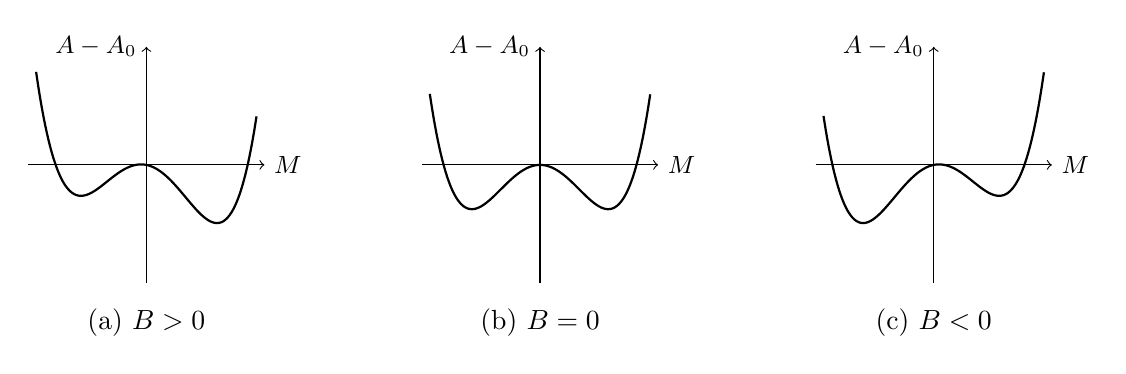
\begin{tikzpicture}
            \draw[->] (-1.5,0)--(1.5,0)node[right]{\small\(M\)};
            \draw[->] (0,-1.5)--(0,1.5)node[left]{\small\(A-A_0\)};
            \draw[thick, domain=-1.4:1.4,samples=100, smooth, variable=\x] plot ({\x}, {-0.2*\x-1.5*\x*\x+\x*\x*\x*\x});
            \node at (0,-2) {(a) \(B>0\)};
            \draw[->] (3.5,0)--(6.5,0)node[right]{\small\(M\)};
            \draw[->] (5,-1.5)--(5,1.5)node[left]{\small\(A-A_0\)};
            \draw[thick, domain=-1.4:1.4,samples=100, smooth, variable=\x] plot ({\x+5}, {-1.5*\x*\x+\x*\x*\x*\x});
            \node at (5,-2) {(b) \(B=0\)};
            \draw[->] (8.5,0)--(11.5,0)node[right]{\small\(M\)};
            \draw[->] (10,-1.5)--(10,1.5)node[left]{\small\(A-A_0\)};
            \draw[thick, domain=-1.4:1.4,samples=100, smooth, variable=\x] plot ({\x+10}, {0.2*\x-1.5*\x*\x+\x*\x*\x*\x});
            \node at (10,-2) {(c) \(B<0\)};
        \end{tikzpicture}
        \caption{The Landau free energy of Ising model with non-zero magnetic fields at low temperatures for different magnetic fields.}
    \end{figure}

    At very high temperature, the double well potential is lost in favour of a single minimum. There is a unique ground state, albeit shifted from \(M=0\) by the presence of the linear term \(a(T,B)\) in the expansion above (which translates into the magnetic field \(B\) in the Ising model). The temperature at which the metastable ground state of the system is lost corresponds to the spinodal point in our discussion of the liquid-gas transition. This time, when we switch the direction of the magnetic field, no phase transition will occur, and similarly when the magnetic field is non-zero, there will be no phase transition as we change the temperature.

    \begin{figure}
        \centering
        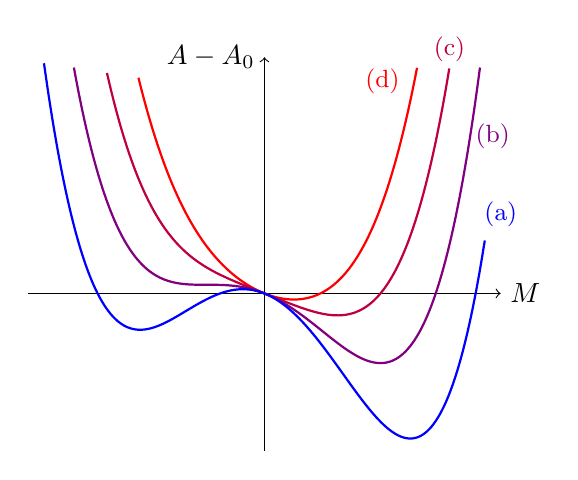
\begin{tikzpicture}
            \draw[->] (-3,0)--(3,0)node[right]{\(M\)};
            \draw[->] (0,-2)--(0,3)node[left]{\(A-A_0\)};
            \draw[thick, red, domain=-0.8:0.97,samples=100, smooth, variable=\x] plot ({2*\x}, {-0.8*\x+2*\x*\x+2*\x*\x*\x*\x});
            \draw[thick, purple, domain=-1:1.175,samples=100, smooth, variable=\x] plot ({2*\x}, {-0.8*\x+2*\x*\x*\x*\x});
            \draw[thick, violet, domain=-1.21:1.37,samples=100, smooth, variable=\x] plot ({2*\x}, {-0.8*\x-1.63*\x*\x+2*\x*\x*\x*\x});
            \draw[thick, blue, domain=-1.4:1.4,samples=100, smooth, variable=\x] plot ({2*\x}, {-0.8*\x-3*\x*\x+2*\x*\x*\x*\x});
            \node[blue] at (3,1) {\small (a)};
            \node[violet] at (2.9,2) {\small (b)};
            \node[purple] at (2.35,3.1) {\small (c)};
            \node[red] at (1.5,2.7){\small (d)};
        \end{tikzpicture}
        \caption{The Landau free energy of an Ising model with non-zero magnetic field as temperature changes. (a) The temperature is low and the free energy curve shows a double well. (b) This is the spinodal where the metastable state disappears. (c) This is the phase transition temperature when \(B=0\). Above this temperature, there will be no phase transition as we change \(B\). (d) This is the high temperature case.}
    \end{figure}

    It is worth noticing that although Landau theory is a simple and useful way of analysing phase transitions, it is not rigorous. In particular, it makes the assumption that the state of a system is completely determined by the minimum of the Landau free energy. However, as we have seen before, fluctuations about the minimum are crucial in phase transitions. This problem can be fixed by a more advanced theory called Landau--Ginzburg theory, which you can find in appendix \cref{Chap:Landau_Ginzburg}.

    \begin{figure}
        \centering
        \begin{tikzpicture}
            \draw[->] (0,0)--(4,0)node[right]{\(T\)};
            \draw[->] (0,-2)--(0,2)node[left]{\(B\)};
            \draw[red,thick] (0,0)--(2,0);
            \draw[fill=red,red] (2,0)node[below,black]{\(T_{\text{ch}}\)} circle (0.05);
        \end{tikzpicture}
        \caption{The phase diagram of the Ising model.}
    \end{figure}

    \newpage
    \section{Transport Phenomena}
    \subsection{Diffusion and Einstein Relation}
    At non-zero temperatures, molecules are always in motion. If they are in liquid or gas phase where there are enough translational degrees of freedom, they will move and collide frequently and as a result, follow highly irregular trajectories that are often called \textit{random walks}. It is difficult to observe the thermal motion of molecules directly, but large particles also undergo thermal motion. The most famous example is the Brownian motion, which was discovered by Robert Brown and was first rationalised by Albert Einstein. This random motion of molecules is responsible for the process that we call \textit{diffusion}. If we carefully introduce a small droplet of ink into a glass of water, then even without stirring, the droplet will become increasingly fuzzy until the colour is uniform in the water. The initial inhomogeneities are washed out over time.

    In what follows, we will consider the simplest type of diffusion known as \textit{self-diffusion}. This is when the diffusing molecules move in a medium consisting of the same species. In experiment, we can study self-diffusion if we can label some of the molecules without affecting their interactions with the others by controlling their nuclear spins or isotopic composition.

    The macroscopic law that describes diffusion is \textit{Fick's first law}. It states that whenever there is a local concentration gradient of some species, then there will be a flux \(\vb{j}\) proportional to the negative of the concentration gradient. In one dimension, if the concentration of some species at a point \(x\) at time \(t\) is \(c(x,t)\), then there will be a flux of the species given by
    \begin{equation}
        j(x,t)=-D\pdv{c}{x}\,,
    \end{equation}
    where the constant of proportionality \(D\) is known as the \textit{diffusion coefficient}.

    Now consider a small region between \(x\) and \(x+\delta x\). The change in the number of the species of interest over a small time interval \(\delta t\) is
    \begin{equation}
        \delta N=N_{\text{in}}-N_{\text{out}}=[j(x)-j(x+\delta x)]\delta t\,.
    \end{equation}
    By the definition of concentration in one dimension, we have
    \begin{align}
        \pdv{c}{t}&=\lim_{\delta t\to 0}\frac{\delta c}{\delta t}=\lim_{\delta t\to 0}\lim_{\delta x\to 0}\frac{\delta N}{\delta x\delta t}\notag\\
        &=-\lim_{\delta x\to 0}\frac{j(x+\delta x)-j(x)}{\delta x}\notag \\
        &=-\pdv{j}{x}\,.
    \end{align}
    From this, we get \textit{Fick's second law}
    \begin{equation}
        \pdv{c}{t}=D\pdv[2]{c}{x}\,,
    \end{equation}
    which is also known as the \textit{diffusion equation} in one dimension.

    This is a second-order linear partial differential equation. It is not difficult to solve. A particularly important case is when the initial condition is the Dirac delta function \(c(x,0)=\delta(x)\). Then the solution is given by
    \begin{equation}
        c(x,t)=\frac{1}{(4\pi Dt)^{1/2}}\exp\left(-\frac{x^2}{4Dt}\right)\,.
    \end{equation}
    This is a Gaussian of width increasing with time. However, in this course, we will not need to solve this diffusion equation directly. Instead, we just want to find out time dependence of the mean squared width of a concentration profile,
    \begin{equation}
        \eval{x^2(t)}=\int\dd{x}x^2c(x,t)\,,
    \end{equation}
    where we have assumed the concentration is normalised
    \begin{equation}
        \int\dd{x}c(x,t)=1
    \end{equation}
    so that the total particle number of the diffusion species we are interested in is always unity. We can multiply the diffusion equation by \(x^2\) and integrate to get
    \begin{equation}
        \int\dd{x}x^2\pdv{c}{t}=D\int\dd{x}x^2\pdv[2]{c}{x}\,.
    \end{equation}
    We can move the differentiation with respect to \(t\) outside of the integration by the Leibniz integral rule, giving
    \begin{equation}
        \pdv{}{t}\int\dd{x}x^2c\equiv\pdv{}{t}\eval{x^2(t)}=D\int\dd{x}x^2\pdv[2]{c}{x}\,.
    \end{equation}
    We can apply integration by parts twice to the right-hand side to get
    \begin{equation}
        \pdv{\eval{x^2}}{t}=D\left[x^2\pdv{c}{x}\right]_{-\infty}^{\infty}-2D\left[xc\right]_{-\infty}^{\infty}+2D\int\dd{x}c(x,t)\,.
    \end{equation}
    If the concentration and its derivative decay fast enough,\footnote{The concentration should decay faster than \(x^{-1}\) in order for the \(\int\dd{x}c\) to converge, and so these boundary terms should vanish.} like in the delta function case where \(c\) decays as a Gaussian, then the previous two boundary terms vanish, and we get
    \begin{equation}\label{Einstein_relation}
        \pdv{\eval{x^2(t)}}{t}=2D\,,
    \end{equation}
    or equivalently
    \begin{equation}
        \eval{x^2(t)}=2Dt\,.
    \end{equation}
    This is the \textit{Einstein relation}, relating the diffusion coefficient \(D\) to the width of the concentration profile. This can easily be generalised to 3D systems to give
    \begin{equation}
        \eval{\vb{x}^2(t)}=6Dt\,.
    \end{equation}
    It should be realised that, whilst \(D\) is a macroscopic transport coefficient, \(\eval{\vb{x}^2}\) has a microscopic interpretation: it is the mean squared distance over which the labelled molecules have moved in a time interval \(t\). If we can follow the motion of individual molecules, we can then determine \(D\) from a knowledge of the particle trajectories.

    \subsection{Random Walk Model of Diffusion}
    Let's consider a simplified model of diffusion, in which both space and time are discretised. We assume that the particles live on an infinite 1D array of points, and they jump to a neighbouring point at a rate \(\Gamma\) per unit time. At every jump, the particle will move a distance \(\ell\), either to the left or to the right, with equal probability, and the direction of each jump is independent. Then the average distance of each jump is
    \begin{equation}
        \eval{\Delta x_1}=0.5\times\ell-0.5\times\ell=0
    \end{equation}
    as one might expect from symmetry: the particles do not move on average. However, the mean squared displacement of the particle after one jump is non-zero,
    \begin{equation}
        \eval{(\Delta x_1)^2}=0.5\times\ell^2+0.5\times (-\ell)^2=\ell^2\,.
    \end{equation}
    Now let's consider what will happen after time \(t\). By then, the molecule will have attempted \(M=\Gamma t\) jumps on average, and the mean displacement will be
    \begin{equation}
        \eval{\Delta x}=\eval{\sum_{i=1}^{M}\Delta x_i}=\sum_{i=1}^{M}\eval{\Delta x_i}=0\,,
    \end{equation}
    where \(\Delta x_i\) is the displacement of the \(i^{\text{th}}\) jump. Next, we have
    \begin{equation}
        \eval{x^2(t)}=\eval{\left(\sum_{i=1}^{M}\Delta x_i\right)^2}=\eval{\sum_{i=1}^{M}\sum_{j=1}^{M}\Delta x_i\Delta x_j}=\sum_{i=1}^{M}\sum_{j=1}^{M}\eval{\Delta x_i\Delta x_j}\,.
    \end{equation}
    As different jumps are uncorrelated, we have
    \begin{equation}
        \eval{\Delta x_i\Delta x_j}=\frac{1}{4}[\ell\times\ell+\ell\times(-\ell)+(-\ell)\times \ell+(-\ell)\times(-\ell)]=0
    \end{equation}
    for \(i\ne j\), while if \(i=j\), \(\eval{\Delta x_i\Delta x_j}=\eval{(\Delta x_i)^2}=\ell^2\). Therefore,
    \begin{equation}
        \eval{x^2(t)}=\sum_{i=1}^{M}\eval{(\Delta x_i)^2}=M\ell^2=\Gamma t\ell^2\,.
    \end{equation}
    
    We can relate this to the Einstein relation
    \begin{equation}
        \pdv{\eval{x^2(t)}}{t}=2D\,,
    \end{equation}
    and so we get the diffusion coefficient for a random walk model
    \begin{equation}
        D=\frac{1}{2}\Gamma \ell^2\,.
    \end{equation}
    This relates the macroscopic diffusion coefficient \(D\) to the microscopic jump frequency \(\Gamma\) and jump distance \(\ell\).

    We can use this to model the diffusion of gas molecules in 3D. If the molecules move at a typical thermal speed \(v\) between collisions, and the mean free path between collisions is \(\lambda\) (both of which can be obtained from kinetic theory), then we can model the movement of a molecule between each collision as a single jump in random walk, with mean jump distance in any direction given by\footnote{We have a factor \(\frac{1}{3}\) because the walk is in three dimensions, which probably does not matter for an order-of-magnitude estimate.}
    \begin{equation}
        \ell^2\approx\frac{\lambda^2}{3}
    \end{equation}
    and mean jumping rate
    \begin{equation}
        \Gamma\approx\frac{v}{\lambda}\,.
    \end{equation}
    Then the diffusion coefficient can be estimated to be
    \begin{equation}
        D=\frac{1}{2}\Gamma\ell^2\approx\frac{1}{6}v\lambda\,.
    \end{equation}

    \subsection{The Green--Kubo Relation}
    The above random walk is a highly simplified model. Molecules in liquid and gas do not move by jumps. Rather, their velocity changes continuously in time. If a molecule has an initial \(x\)-velocity \(v_x(0)\) at time \(t=0\), then its velocity will still be close to \(v_x(0)\) at a short time afterwards before it collides with another molecule. `Short' in this context depends on the conditions. For a water molecule at room temperature, it takes around \(10^{-13}\unit{s}\) before a molecule forgets about its initial velocity.

    The displacement \(\Delta\vb{r}(t)\) that we are interested in is simply the time integral of the velocity of the labelled particle,
    \begin{equation}
        \Delta\vb{r}(t)=\int_{0}^{t}\dd{t'}\vb{v}(t')\,.
    \end{equation}
    The Einstein relation (\ref{Einstein_relation}) allows us to relate the diffusion coefficient in terms of the particle velocities, so we start from
    \begin{equation}
        D=\frac{1}{2}\lim_{t\to\infty}\pdv{\eval{x^2(t)}}{t}\,,
    \end{equation}
    where we have only considered the \(x\) component of the mean squared displacement for convenience.\footnote{We set the limit \(t\to\infty\) to ensure the motion of the molecule is diffusive rather than ballistic. You can see more on this discussion in one of the exercises.} We can write \(x(t)\) as the time integral of the \(x\)-component of the labelled particle velocity, so
    \begin{equation}
        \eval{x^2(t)}=\eval{\left(\int_{0}^{t}\dd{t}v_x(t')\right)^2}=\int_{0}^{t}\dd{t'}\int_{0}^{t}\dd{t''}\eval{v_x(t')v_x(t'')}\,.
    \end{equation}
    The quantity \(\eval{v_x(t')v_x(t'')}\) is called the \textit{velocity autocorrelation function}. It measures the average correlation between the velocity of a particle at times \(t'\) and \(t''\). A typical velocity autocorrelation function is shown in \cref{autocorrelation}.

    \begin{figure}
        \centering
        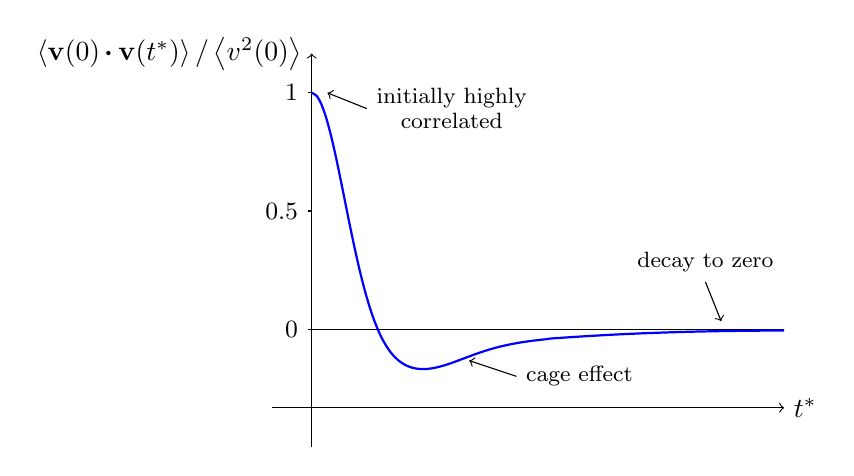
\begin{tikzpicture}
            \draw[->] (-0.5,0)--(6,0)node[right]{\(t^*\)};
            \draw[->] (0,-0.5)--(0,4.5)node[left]{\(\eval{\vb{v}(0)\vdot\vb{v}(t^*)}/\eval{v^2(0)}\)};
            \draw (0,1)--(-0.05,1)node[left]{\small\(0\)};
            \draw (0,2.5)--(-0.05,2.5)node[left]{\small\(0.5\)};
            \draw (0,4)--(-0.05,4)node[left]{\small\(1\)};
            \draw (0,1)--(6,1);
            \draw[thick, blue, domain=0:6,samples=100, smooth, variable=\x] plot ({\x}, {1+3.3*2.72^(-3*\x*\x)-0.5*\x*\x*\x*\x*2.72^(-\x*\x)-0.3*2.72^(-0.1*\x*\x)});
            \draw[->] (0.7,3.8)node[right,align=center]{\footnotesize initially highly \\[-3pt] \footnotesize correlated}--(0.2,4);
            \draw[->] (2.6,0.4)node[right]{\footnotesize cage effect}--(2,0.6);
            \draw[->] (5,1.6)node[above]{\footnotesize decay to zero}--(5.2,1.1);
        \end{tikzpicture}
        \caption{A schematic plot of velocity autocorrelation functions for liquid. For short time \(t^*\), the velocity is highly correlated to its initial value since the velocity of a particle does not change significantly before colliding with another particle. In a liquid, particles are often surrounded by a cage of other particles, and so we often see an anti-correlation after a short time, where the particle has bounced back after hitting the cage and is travelling in the opposite direction from the one it started with. In the long time limit, the particle has collided with many other particles, which has effectively randomised its velocity vector, so it is no longer correlated with the initial value. The velocity autocorrelation function decays to zero.}
        \label{autocorrelation}
    \end{figure}

    We can simplify this integral
    \begin{align}
        \eval{x^2(t)}&=\int_{0}^{t}\dd{t'}\int_{0}^{t'}\dd{t''}\eval{v_x(t')v_x(t'')}+\int_{0}^{t}\dd{t'}\int_{t'}^{t}\dd{t''}\eval{v_x(t')v_x(t'')}\notag \\
        &=\int_{0}^{t}\dd{t'}\int_{0}^{t'}\dd{t''}\eval{v_x(t')v_x(t'')}+\int_{0}^{t}\dd{t''}\int_{0}^{t''}\dd{t'}\eval{v_x(t')v_x(t'')}\notag \\
        &=2\int_{0}^{t}\dd{t'}\int_{0}^{t'}\dd{t''}\eval{v_x(t')v_x(t'')}\,.
    \end{align}
    The velocity autocorrelation function is an equilibrium property of the system, since it describes the average correlation between velocities at different times along an equilibrium trajectory. As equilibrium properties are time invariant, we can shift the time origin by an arbitrary amount \(\Delta t\), so that
    \begin{equation}
        \eval{v_x(t')v_x(t'')}=\eval{v_x(t'+\Delta t)v_x(t''+\Delta t)}\,.
    \end{equation}
    We therefore have
    \begin{equation}
        \eval{v_x(t')v_x(t'')}=\eval{v_x(t'-t'')v_x(0)}\,,
    \end{equation}
    so
    \begin{equation}
        \eval{x^2(t)}=2\int_{0}^{t}\dd{t'}\int_{0}^{t'}\dd{t''}\eval{v_x(t'-t'')v_x(0)}\,.
    \end{equation}
    Finally using the Einstein relation, we can write
    \begin{align}
        D&=\lim_{t\to\infty}\pdv{}{t}\int_{0}^{t}\dd{t'}\int_{0}^{t'}\dd{t''}\eval{v_x(t'-t'')v_x(0)}\notag\\
        &=\lim_{t\to\infty}\int_{0}^{t}\dd{t''}\eval{v_x(t-t'')v_x(0)}\,.
    \end{align}
    By introducing the variable \(\tau=t-t''\), we have
    \begin{equation}
        D=\int_{0}^{\infty}\dd{\tau}\eval{v_x(\tau)v_x(0)}
    \end{equation}
    known as the \textit{Green--Kubo relation}, which relates the diffusion coefficient \(D\) to the velocity autocorrelation function. In an isotropic 3D system, this becomes
    \begin{equation}
        D=\frac{1}{3}\int_{0}^{\infty}\dd{\tau}\eval{\vb{v}(\tau)\vdot\vb{v}(0)}\,.
    \end{equation}
    
    More generally, a Green--Kubo relation is any equation that relates an integral of a time-correlation function to a transport coefficient, such as shear viscosity, thermal conductivity and electrical conductivity \textit{etc.} It should be emphasised that for classical systems, the Green--Kubo relation for \(D\) and the Einstein relation \(\eval{x^2}=2Dt\) are strictly equivalent.
    \subsection{Langevin Equation and Stokes--Einstein Relation}
    The Green--Kubo expression for the diffusion coefficient provides a way of estimating the diffusion coefficient of particles dissolved in viscous fluid, since in such cases, we can make a few reasonable assumptions to compute the velocity autocorrelation function. In particular, we will assume the following:
    \begin{itemize}
        \item When a particle is subjected to a constant external force \(\vb{F}\), the average drift velocity will be given by
        \begin{equation}
            \eval{\vb{v}}=\frac{\vb{F}}{\gamma}\,,
        \end{equation}
        where \(\gamma\) is the \textit{friction coefficient}, and a related quantity is \(\mu=1/\gamma\) known as the \textit{mobility}.
        \item If you put some fluid between two parallel plates of area \(A\) separated by \(h\) and move the two plates relative to each other with constant relative velocity \(v\), then usually there will be a constant velocity gradient
        \begin{equation}
            \pdv{u}{z}=\frac{v}{h}
        \end{equation}
        within the fluid. The magnitude of the force \(F\) that has to be exerted on the top plate to maintain the relative motion is given by
        \begin{equation}
            F=\eta A\frac{v}{h}\,,
        \end{equation}
        where the constant of proportionality \(\eta\) is known as the \textit{viscosity}. We will assume that our fluid has a constant viscosity \(\eta\).
        \item For a spherical particle with a radius \(a\) moving in a fluid with viscosity \(\eta\), we can approximate the friction coefficient \(\gamma\) by the \textit{Stokes expression}
        \begin{equation}
            \gamma=6\pi\eta a\,.
        \end{equation}
        This assumes no slippage of the fluid at the surface of the sphere.
        \item The particles experience random collisions with their neighbours. The effect of these collisions is to exert a random force \(F^R(t)\) on our particle. We will assume that \(F^R(t)\) for \(t>0\) is not correlated with the velocity of the particle at time \(t=0\).
    \end{itemize}

    \begin{figure}
        \centering
        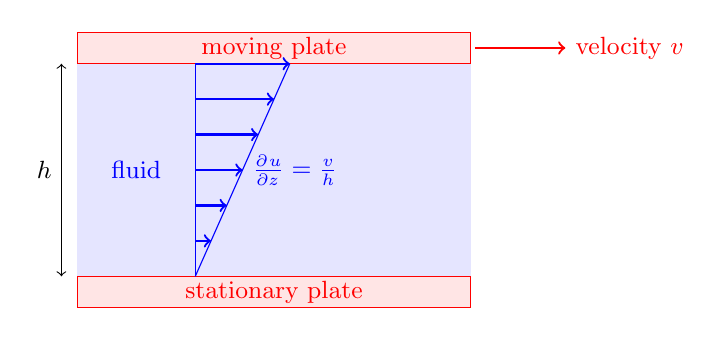
\begin{tikzpicture}
            \fill[blue!10] (0,0.4) rectangle (5,3.1);
            \draw[red,fill=red!10] (0,0) rectangle (5,0.4);
            \draw[red,fill=red!10] (0,3.1) rectangle (5,3.5);
            \node[red] at (2.5,0.2) {\small stationary plate};
            \node[red] at (2.5,3.3) {\small moving plate};
            \draw[->,red,thick] (5.05,3.3)--(6.2,3.3)node[right,red]{\small velocity \(v\)};
            \draw[<->] (-0.2,0.4)--node[left]{\small\(h\)}(-0.2,3.1);
            \node[blue] at (0.75,1.75) {\small fluid};
            \draw[blue] (1.5,0.4)--(1.5,3.1);
            \foreach \x in {1,...,6}{
                \draw[->,thick,blue] (1.5,0.4+0.45*\x)--(1.5+0.2*\x,0.4+0.45*\x);
            }
            \draw[blue](1.5,0.4)--node[right]{\small\(\pdv{u}{z}=\frac{v}{h}\)}(2.7,3.1);
        \end{tikzpicture}
        \caption{When two parallel plates filled with fluid are moving with relative velocity \(v\), the retarding force will be proportional to both the area of the plates and the velocity gradient, with proportionality constant known as the viscosity. To avoid boundary effects in experiments, this is usually done using rotating discs.}
    \end{figure}

    For simplicity, we again only consider the \(x\) component of the motion. The above assumptions allow us to write, by Newton's second law,
    \begin{equation}\label{Langevin}
        m\dot{v}_x(t)+\gamma v_x(t)=F_x^R(t)\,.
    \end{equation}
    This is known as the \textit{Langevin equation}.

    We can multiply both sides of the Langevin equation (\ref{Langevin}) by \(v(0)\) and use the assumption \(\eval{v_x(0)F_x^R(t)}=0\) to obtain the condition of the velocity correlation function
    \begin{equation}
        m\eval{v_x(0)\dot{v}_x(t)}+\gamma\eval{v_x(0)v_x(t)}=0\,.
    \end{equation}
    This is an easy ordinary differential equation with solution
    \begin{equation}
        \eval{v_x(0)v_x(t)}=\eval{v_x(0)^2}\exp\left(-\frac{\gamma t}{m}\right)\,.
    \end{equation} 
    At equilibrium, the velocities of the particles are distributed according to the Maxwell distribution, with \(\eval{v_x^2(0)}=k_B T/m\).\footnote{Or, equally well, by the equipartition of energy.} We then have
    \begin{equation}
        D=\int_{0}^{\infty}\dd{t}\frac{k_B T}{m}\exp\left(-\frac{\gamma t}{m}\right)=\frac{k_B T}{\gamma}\,.
    \end{equation}
    If we use the Stokes approximation for \(\gamma\), we get
    \begin{equation}
        D=\frac{k_B T}{6\pi\eta a}\,,
    \end{equation}
    known as the \textit{Stokes--Einstein relation}. It is extremely useful and it correctly reproduces the experimental fact that for many liquids, the product \(D\eta\) is very nearly proportional to the temperature, even when \(D\) and \(\eta\) each vary orders of magnitude. It is also a good way to determine Boltzmann's constant experimentally. The experiment was done in 1909 by Jean-Baptiste Perrin and won him the 1926 Nobel prize.

    The Stokes--Einstein relation actually has profound implications. It tells us diffusion and viscosity are closely related --- their microscopic origins are both the random bombardment of molecules. It is also an important example of the fluctuation-dissipation theorem. The fluctuations of the particle as it undergoes its random walk are related to the drag force (or dissipation of momentum) that the particle feels as it moves through the fluid.

    \subsection{The Einstein--Smoluchowski Relation}\label{Chap:Einstein_Smoluchowski}
    There is another more general way of deriving the relation between the mobility and the diffusion coefficient \(D\). Consider a solution in a closed volume \(V\). If there is a concentration gradient of the dissolved species, then this will result in a diffusion flux \(\vb{j}\) as predicted by Fick's first law. The diffusive flux equals the product of the number density and the average drift velocity of these particles,
    \begin{equation}
        \vb{j}=\rho\eval{\vb{v}}\,.
    \end{equation}
    Now suppose that the dissolved particles are subject to an external potential \(U(x)\). If this potential is not constant, then there will be a net force acting on the particles, given by
    \begin{equation}
        f_x=-\pdv{U(x)}{x}\,,
    \end{equation}
    where we have again reduced the problem to one dimension for simplicity. The average drift velocity of a particle due to this force is
    \begin{equation}
        \eval{v_x}=\mu f_x=-\mu\pdv{U(x)}{x}\,.
    \end{equation}
    As the particles move under the influence of this force, the density becomes inhomogeneous. But if the particle number density is not constant, there is also a diffusion flux. When the system reaches equilibrium, the flux due to diffusion and the flux due to external force will balance
    \begin{equation}
        0=j_{\text{tot}}=\rho(x)\eval{v_x}-D\pdv{\rho(x)}{x}=-\rho(x)\mu\pdv{U(x)}{x}-D\pdv{\rho(x)}{x}\,.
    \end{equation}
    At equilibrium, the probability of finding a particle at a position \(x\) for an inhomogeneous system is proportional to the Boltzmann factor,
    \begin{equation}
        \rho(x)=\rho_0\exp\left(-\frac{U(x)}{k_B T}\right)\,.
    \end{equation}
    Therefore, we have
    \begin{equation}
        -\rho(x)\mu\pdv{U(x)}{x}+\frac{D}{k_B T}\rho(x)\pdv{U(x)}{x}=0\,.
    \end{equation}
    This equation is satisfied for all \(x\) if
    \begin{equation}
        \mu=\frac{D}{k_B T}\,,
    \end{equation}
    which is known as the \textit{Einstein--Smoluchowski relation}. We have recovered the same expression as obtained from the Langevin equation, but we have made fewer assumptions along the way. Moreover, this approach is more easily generalisable to include external fields.

    A more systematic, formal approach to fluctuation-dissipation relations and the link between transport coefficients and equilibrium statistical mechanics is explored in appendix \cref{Chap:Intro_to_Linear_Response}

    \newpage
    \section{Polymers}
    In the last chapter, we found that the distribution of displacements of particles under diffusion is given by a Gaussian function. Rather interestingly, the same distribution describes the end-to-end distance of a polymer chain consisting of non-interacting segments. The similarity is more than superficial: it arises from the random walk nature of both phenomena.
    \subsection{Size of an Ideal Polymer}
    Let's consider a polymer that consists of \(N\) segments of length \(\ell\). When the polymer is fully stretched into a straight line, the total length of the polymer chain is
    \begin{equation}
        R_c=N\ell\,,
    \end{equation}
    known as the \textit{contour length} of the polymer. However, a real polymer molecule is rarely completely straight: when it coils up, its size will be less than \(R_c\). We will model the polymer as fully flexible, so that every segment can rotate freely around its connecting point to the previous segment. Of course this is a huge simplification, but in practice, many polymers do behave like a freely joined chain, although the length \(\ell\) is larger than the size of a monomer --- it is the length at which the orientation of the polymer chain becomes uncorrelated. In addition, we will make the assumption that the polymer is \textit{ideal}, such that different segments do not interact. We have seen that under \(\theta\) conditions, the polymer segments do behave ideally, and this can be used as a rough estimate of the behaviour of non-ideal polymers.

    We want to find out the average \textit{end-to-end} distance of an ideal polymer. If we denote the vector pointing from the beginning to the end point of the \(i^{\text{th}}\) segment by \(\vb{\ell}_i\) such that \(\norm{\vb{\ell}_i}=\ell\), then the total end-to-end vector is
    \begin{equation}
        \vb{R}_{\text{ee}}=\sum_{i=1}^{N}\vb{\ell}_i\,.
    \end{equation}
    We would like to compute its average. However, by symmetry, a polymer segment has equal probability to point in any orientation, so \(\eval{\vb{\ell}_i}=\vb{0}\). As a result, the average end-to-end distance of a polymer is
    \begin{equation}
        \eval{\vb{R}_{\text{ee}}}=\eval{\sum_{i=1}^{N}\vb{\ell}_i}=\sum_{i=1}^{N}\eval{\vb{\ell}_i}=\vb{0}
    \end{equation}
    as one might predict by symmetry. Just like in the case of diffusion, a better measure for the size of a coiled ideal polymer is the \textit{mean squared end-to-end distance} \(\eval{\vb{R}_{\text{ee}}^2}\),
    \begin{align}
        \eval{\vb{R}_{\text{ee}}^2}&=\eval{\left(\sum_{i=1}^{N}\vb{\ell}_i\right)^2}=\eval{\left(\sum_{i=1}^{N}\vb{\ell}_i\right)\vdot\left(\sum_{i=1}^{N}\vb{\ell}_i\right)}\notag \\
        &=\eval{\sum_{i,j=1}^{N}\vb{\ell}_i\vdot\vb{\ell}_j}=\sum_{i,j=1}^{N}\eval{\vb{\ell}_i\vdot\vb{\ell}_j}=\ell^2\sum_{i,j=1}^{N}\eval{\cos\theta_{ij}}\,.
    \end{align}
    For different segments \(i\ne j\), the orientations are uncorrelated, so \(\eval{\cos\theta_{ij}}=0\). However, for \(i=j\), \(\theta_{ij}=0\) and hence \(\cos\theta_{ii}=1\). As a consequence, all the cross-terms with \(i\ne j\) vanish and we have
    \begin{equation}
        \eval{\vb{R}_{\text{ee}}^2}=N\ell^2\,.
    \end{equation}
    The root mean squared end-to-end distance is therefore
    \begin{equation}
        \sqrt{\eval{\vb{R}_{\text{ee}}^2}}=\sqrt{N}\ell\,.
    \end{equation}
    \subsection{Probability Distribution for the End-to-End Distance}
    We can actually do better than simply calculating the mean squared end-to-end distance of a polymer: we can actually compute the probability distribution of \(\vb{R}_{\text{ee}}\). However, to simplify matters, we will only consider the one-dimensional case. Again, consider \(N\) freely joined segments of length \(\ell\). We denote the number of segments pointing right by \(N_R\), and the number pointing to the left by \(N_L\). We denote their difference \(N_R-N_L\eqqcolon D\) and clearly the end-to-end distance is \(X_{\text{ee}}=D\ell\). We can compute the probability of finding the chain in a conformation with a given value of \(D\). The total number of conformations of \(N\) polymer segments is \(2^N\), and the number of ways in which we can have \(N_R\) segments pointing to the right and \(N_L\) segments pointing to the left is
    \begin{equation}
        \Omega(N_R,N_L)=\frac{N!}{N_R!N_L!}=\frac{N!}{[\frac{1}{2}(N+D)]![\frac{1}{2}(N-D)]!}\,.
    \end{equation}
    Hence, the probability of having a conformation with some \(D\) is
    \begin{equation}
        \Prob(N,D)=\frac{N!}{[\frac{1}{2}(N+D)]![\frac{1}{2}(N-D)]!}\left(\frac{1}{2}\right)^N\,.
    \end{equation}
    We can expand this using Stirling's approximation
    \begin{equation}
        \ln x!=x\ln x-x+\ln\sqrt{2\pi x}+O\left(\frac{1}{x}\right)
    \end{equation}
    to get
    \begin{align}
        \ln \Prob(N,D)=-\frac{1}{2}N&\ln\left(1-\frac{D^2}{N^2}\right)+\ln\sqrt{2\pi N}\notag\\
        &-\ln\sqrt{\pi(N+D)}-\ln\sqrt{\pi(N-D)}-\frac{1}{2}D\ln\left(\frac{1+\frac{D}{N}}{1-\frac{D}{N}}\right)
    \end{align}
    for large \(N\). For \(D/N\ll 1\), we can use Taylor expansion \(\ln(1\pm x)=\pm x+O(x^2)\) when \(\abs{x}\ll 1\) to write
    \begin{equation}
        \ln\Prob(N,D)\approx -\frac{D^2}{2N}-\ln\sqrt{\pi N/2}\,,
    \end{equation}
    from which we have
    \begin{equation}
        \Prob(N,D)=\frac{1}{\sqrt{\pi N/2}}\exp\left(-\frac{D^2}{2N}\right)\,.
    \end{equation}
    However, if you try to integrate this expression, you will find that this is not properly normalised:
    \begin{equation}
        \int_{-\infty}^{\infty}\dd{D}\Prob(D,N)=2\,.
    \end{equation}
    What is wrong with this expression? Notice that if in order to keep \(N_R+N_L=N\) fixed, if \(N_R\) increases by 1, then \(N_L\) should decrease by 1 --- this leads to a change in \(D\) by 2. When \(N\) is even, then \(D\) can only be even, and if \(N\) is odd, then \(D\) can only be odd. This means that half of the probability distribution of \(D\) should actually be 0.
    \begin{equation}
        \Prob(N,D)=\begin{cases}
            \frac{1}{\sqrt{\pi N/2}}\exp\left(-\frac{D^2}{2N}\right) & \text{if } N\equiv D\,(\mathrm{mod}\, 2)\\
            0 & \text{otherwise\,.}
        \end{cases}
    \end{equation}
    However, in practice, it is more often to just halve the probability density and write
    \begin{equation}
        \Prob(D)=\frac{1}{\sqrt{2\pi N}}\exp\left(-\frac{D^2}{2N}\right)
    \end{equation}
    so that it is properly normalised and gives the probability of \(D\) being in some interval from \(D\) to \(D+\Delta D\) correctly when \(N\) is large so that we can effectively treat \(D\) as a continuum. From this Gaussian distribution, we can also deduce the mean squared end-to-end distance of the one-dimensional chain to be
    \begin{equation}\label{polymer_rms_distance}
        \eval{X_{\text{ee}}^2}=\ell^2\eval{D^2}=N\ell^2
    \end{equation}
    as obtained previously.

    \subsection{Thermodynamics of Ideal Polymers}
    Finally we can make a link to the thermodynamics. From the statistical mechanical definition of the entropy, we have
    \begin{equation}
        S(D)=-\frac{D^2 k_B}{2N}+\text{const.}
    \end{equation}
    where const. accounts for all terms that are independent of \(D\). This expression is valid for small \(D\). The end-to-end elongation of the polymer is \(X_{\text{ee}}=D\ell\), so the entropy of a polymer chain with end-to-end distance \(X_{\text{ee}}\) is
    \begin{equation}
        S(X_{\text{ee}})=-\frac{X_{\text{ee}}^2 k_B}{2N\ell^2}+\text{const.}
    \end{equation}
    Since the polymer is ideal, there is no energetic preference for any value of \(X_{\text{ee}}\), and the internal energy \(E\) only depends on the temperature, just as for an ideal gas. By the first law of thermodynamics,
    \begin{equation}
        \d{E}=\dbar w+\dbar q\,.
    \end{equation}
    The heat transfer is given by the Clausius expression \(\dbar q=T\d{S}\) and the work done to change the length of a polymer is \(\dbar w=F\d{X_{\text{ee}}}\), where \(F\) is the external force applied to stretch the polymer. We then have
    \begin{equation}
        \d{E}=T\d{S}+F\d{X_{\text{ee}}}\,,
    \end{equation}
    and so at constant temperature,
    \begin{equation}
        \left(\pdv{E}{X_{\text{ee}}}\right)_T=0=T\left(\pdv{S}{X_{\text{ee}}}\right)_T + F\,,
    \end{equation}
    and hence
    \begin{equation}
        F=-T\left(\pdv{S}{X_{\text{ee}}}\right)_T\,.
    \end{equation}
    By our expression of the entropy, we get
    \begin{equation}\label{polymer_force}
        F=\frac{k_B T}{N\ell^2}X_{\text{ee}}\,.
    \end{equation}
    The restoring force \(-F\) is linear in the extension \(X_{\text{ee}}\) when the extension is small: \(X_{\text{ee}}\ll\sqrt{N}\ell\) --- just like a normal spring. But unlike a metal spring, the spring constant is proportional to temperature. This is exactly the force you feel when stretching a polymer, like a rubber band, and rather surprisingly, this force is purely entropic!

    We can combine (\ref{polymer_rms_distance}) and (\ref{polymer_force}) to get an expression of the spring constant of an ideal polymer
    \begin{equation}
        \kappa=\frac{k_B T}{\eval{X_{\text{ee}}^2}}\,.
    \end{equation}
    In the post-lecture question, you will show that this result is actually also valid for non-ideal polymers.

    Finally, let's consider what will happen if we stretch a polymer adiabatically, i.e. without heat exchange to the environment. For a reversible process, this means that the entropy is held constant, as \(\d{q_{\text{rev}}}=T\d{S}\). The internal energy is clearly a function of \(T\) and \(X_{\text{ee}}\), so by chain rule, the total derivative of energy against the extension is
    \begin{equation}
        \left(\pdv{E}{X_{\text{ee}}}\right)_{S}=\left(\pdv{E}{T}\right)_{X_{\text{ee}}}\left(\pdv{T}{X_{\text{ee}}}\right)_{S}+\left(\pdv{E}{X_{\text{ee}}}\right)_{T}\,.
    \end{equation}
    By comparing to the fundamental equation
    \begin{equation}
        \d{E}=T\d{S}+F\d{X_{\text{ee}}}\,,
    \end{equation}
    we have
    \begin{equation}
        \left(\pdv{E}{X_{\text{ee}}}\right)_{S}=F\,,
    \end{equation}
    and we also know that by definition,
    \begin{equation}
        \left(\pdv{E}{T}\right)_{X_{\text{ee}}}=C_{X_{\text{ee}}}\,,
    \end{equation}
    the heat capacity at constant extension. For an ideal polymer, \((\partial E/\partial X_{\text{ee}})_T=0\), and so we have
    \begin{equation}
        \left(\pdv{T}{X_{\text{ee}}}\right)_{S}=\frac{F}{C_{X_{\text{ee}}}}=\frac{k_B T}{C_{X_{\text{ee}}}N\ell^2}X_{\text{ee}}\,.
    \end{equation}
    As the heat capacity is always positive, it follows that the temperature increases when the polymer is stretched adiabatically, and decreases when the polymer is released.



    \newpage
    \part*{Appendices}
    \addcontentsline{toc}{part}{\protect\numberline{}Appendices}
    \appendix

    \section{Thermodynamics}\label{Chap:Thermodynamics}

    Thermodynamics is a remarkable discipline. It provides us with relations between measurable quantities such as \((\partial S/\partial V)_T=(\partial P/\partial T)_V\). These relations are valid for any substance. But, precisely for this reason, thermodynamics contains no information whatsoever about the underlying microscopic structure of a substance. Thermodynamics preceded statistical mechanics and quantum mechanics, yet not a single thermodynamic relation had to be modified in light of these later developments. The reason is simple: thermodynamics is a phenomenological science. It is based on the properties of matter as we observe them, not upon any theoretical ideas that we may have about matter.
    \subsection{The First Law}
    The first law of thermodynamics expresses the empirical observation that energy is conserved, even though it can be converted into various forms. The internal energy of a system can be changed by either performing work on the system or by transferring an amount of heat.
    \begin{law}[First law of thermodynamics]
        Let \(\dbar q\) be the heat transferred to a system and let \(\dbar w\) be the work done to the system. Then the change in the internal energy of the system is given by
        \begin{equation}
            \Delta E=\dbar q+\dbar w\,.
        \end{equation}
    \end{law}
    \subsection{The Second Law}
    The second law is based on experimental observations.
    \begin{law}[Kelvin's second law]
        It is impossible to make an engine that converts heat from a single heat bath (i.e. a large reservoir at equilibrium) into work.
    \end{law}
    This observation is equivalent to another equally empirical observation.
    \begin{law}[Clausius' second law]
        Heat can never flow spontaneously (i.e. without work being performed) from a cold reservoir to a warmer reservoir.
    \end{law}
    This statement is actually a bit more subtle than it seems because, before we have defined temperature, we can only distinguish hotter and colder by looking at the direction of heat flow. What the second law says is that it is never possible to make heat flow spontaneously in the ``wrong'' direction. How do we get from such a seemingly trivial statement to something as abstract as entropy? This is most easily achieved by introducing the concept of a reversible heat engine.
    \subsubsection{Heat Engines}
    A reversible engine is, as the word suggests, an engine that can be operated in reverse. During one cycle (i.e. a sequence of steps that is completed when the engine is returned into its original state), this engine takes in an amount of heat \(q_1\) from a hot reservoir, converts part of it into work \(w\) and delivers the remaining amount of heat \(q_2\) to a cold reservoir. The reverse process is that, by performing an amount of work \(w\), we can take an amount of heat \(q_2\) from the cold reservoir and deliver an amount of heat \(q_1\) to the hot reservoir. Reversible engines are an idealisation because in any real engine, there will be additional heat losses. However, the ideal reversible engine can be approximated arbitrarily closely by a real engine if, at every stage, the real engine is sufficiently close to equilibrium. As the engine is returned to its original state at the end of one cycle, its internal energy \(E\) has not changed. Hence, the first law tells us that \(\Delta E=q_1-(w+q_2)=0\) or \(q_1=w+q_2\).

    Now consider the efficiency of the engine \(\eta\coloneqq w/q_1\), i.e. the amount of work delivered per amount of heat taken in. At first, one might think that \(\eta\) depends on the precise design of our reversible engine, but this turns out not to be the case: \(\eta\) is the same for all reversible engines operating between the same two reservoirs. To demonstrate this, suppose that we have another reversible engine with efficiency \(\eta'\) that takes in an amount of heat \(q_1'\) from the hot reservoir, delivers the same amount of work \(w\), and then delivers an amount of heat \(q_2'\) to the cold reservoir, as shown in \cref{heat_engines}. Suppose \(\eta\ne\eta'\), then we use the work generated by the engine with the higher efficiency (say \(\eta\)) to drive the second engine (with efficiency \(\eta'\)) in reverse. The amount of heat delivered to the hot reservoir by the second engine is
    \begin{equation}
        q_1'=\frac{w}{\eta'}=\frac{q_1\eta}{\eta'}\,.
    \end{equation}
    As \(\eta'<\eta\) by construction, it follows that \(q_1'>q_1\). Hence there is a net heat flow from the cold reservoir into the hot reservoir, which contradicts the second law of thermodynamics (in the form ``heat can never spontaneously flow from a cold to a hot reservoir''). We have therefore proved by contradiction that the efficiency of all reversible heat engines operating between the same reservoirs is identical.

    \begin{figure}
        \centering
        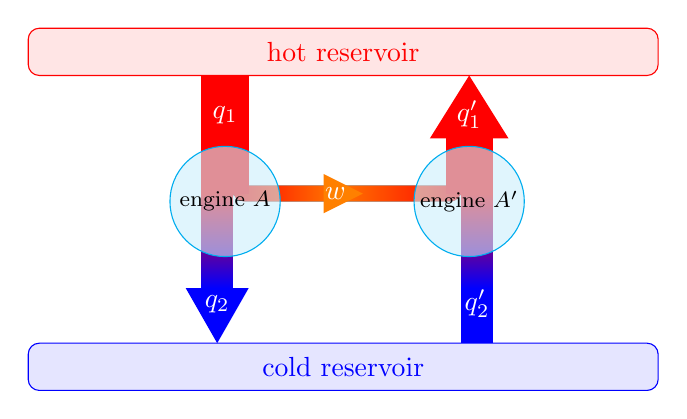
\begin{tikzpicture}
            \draw[blue,fill=blue!10,rounded corners] (0,0) rectangle (8,0.6);
            \node[blue] at (4,0.3) {cold reservoir};
            \draw[red,fill=red!10,rounded corners] (0,4) rectangle (8,4.6);
            \node[red] at (4,4.3) {hot reservoir};
            \fill[left color=red, right color=orange,rounded corners] (2.6,2.6) rectangle (4,2.4);
            \fill[left color=orange, right color=red,rounded corners] (5.5,2.6) rectangle (3.8,2.4);
            \fill[red] (2.2,4) rectangle (2.8,2.5);
            \fill[top color=red,bottom color=blue]  (2.2,2.5) rectangle (2.6,1.3);
            \fill[blue] (2,1.3)--(2.8,1.3)--(2.4,0.6)--(2,1.3);
            \fill[red] (5.6,4)--(6.1,3.2)--(5.1,3.2)--(5.6,4);
            \fill[red] (5.3,3.2) rectangle (5.9,2.5);
            \fill[top color=red, bottom color=blue] (5.5,2.5) rectangle (5.9,1.3);
            \fill[blue] (5.5,1.3) rectangle (5.9,0.6);
            \fill[orange] (3.75,2.25)--(4.25,2.5)--(3.75,2.75)--(3.75,2.25);
            \node[white] at (2.5,3.5) {\(q_1\)};
            \node[white] at (5.6,3.5) {\(q_1'\)};
            \node[white] at (2.4,1.1) {\(q_2\)};
            \node[white] at (5.7,1.1) {\(q_2'\)};
            \node[white] at (3.9,2.5) {\(w\)};
            \draw[cyan,fill=cyan!20,fill opacity=0.6] (2.5,2.4) circle (0.7);
            \node at (2.5,2.4){\footnotesize engine \(A\)};
            \draw[cyan,fill=cyan!20,fill opacity=0.6] (5.6,2.4) circle (0.7);
            \node at (5.6,2.4){\footnotesize engine \(A'\)};
        \end{tikzpicture}
        \caption{If the efficiencies of the two heat engines are not equal, then this setup violates the second law of thermodynamics.}
        \label{heat_engines}
    \end{figure}

    \subsubsection{Absolute Temperatures}
    Since \(\eta\) does not depend on the specific design of a reversible engine, the only variables it can depend on are the temperatures \(t_1\) and \(t_2\) of the reservoirs it connects, i.e. \(\eta=\eta(t_1,t_2)\). We are denoting these temperatures with a lowercase t for the time being because we have not yet defined precisely what we mean by the absolute temperature; the ``temperatures'' defined here merely need to be well-ordered (i.e. monotonic) and serve to identify which reservoir is colder and which is hotter.

    For further convenience, we will also consider the quantity
    \begin{equation}
        R_{12}(t_1,t_2)\coloneqq 1-\eta(t_1,t_2)=\frac{q_1-w}{q_1}=\frac{q_2}{q_1}\,.
    \end{equation}

    Suppose now that we have a reversible engine that consists of two stages: engine 1 working between reservoirs \(A\) and \(B\), and engine 2 working between reservoirs \(B\) and \(C\), as shown in the figure. The three reservoirs are at temperatures \(t_A\), \(t_B\) and \(t_C\), respectively. We have \(R_{AB}\) and \(R_{BC}\)
    \[R_{AB}=\frac{q_{1B}}{q_{1A}}\,,\quad\text{and}\quad R_{BC}=\frac{q_{2C}}{q_{2B}}\,.\]
    Since by construction, the combined engine \(1+2\) is a reversible engine working in two stages, reservoir \(B\) must be neither a source nor a sink of energy, otherwise the overall efficiency of the engine would depend on how many such stages it is made up of, but we saw earlier that the efficiency of every reversible engine is the same. We must therefore conclude that \(q_{1B}=q_{2B}\). The overall value of \(R_{\text{tot}}=1-\eta_{\text{tot}}\) for the combined reversible engine is thus given by
    \begin{equation}
        R_{\text{tot}}=\frac{q_{2C}}{q_{1A}}=R_{AB}R_{BC}\,.
    \end{equation}
    Suppose that in addition, we have another reversible engine, engine 3, that works directly between reservoirs \(A\) and \(C\), with
    \begin{equation}
        R_{AC}=\frac{q_{3C}}{q_{3A}}\,.
    \end{equation}
    Since the engines are reversible, engine 3 and the combined engine \(1+2\) must be equally efficient, as we showed above. This means that
    \begin{equation}
        R_{AB}R_{BC}=R_{AC}\,.
    \end{equation}
    However, recall that these ratios are functions solely of the temperatures of the reservoirs. The right-hand side does not depend on \(t_B\), and so the product of \(R_{AB}\) and \(R_{BC}\) must therefore result in the cancellation of this functional dependence. The above equality can only hold in general provided that
    \begin{equation}
        R_{AB}=\frac{f(t_B)}{f(t_A)}\,,\qquad R_{BC}=\frac{f(t_C)}{f(t_B)}\quad\text{and}\quad R_{AC}=\frac{f(t_C)}{f(t_A)}\,,
    \end{equation}
    where \(f(t)\) is some function of our previously defined temperature \(t\).

    What we do next is to introduce an \textit{absolute} (or \textit{thermodynamic}) \textit{temperature} \(T\) given by \(T=f(t)\) so that
    \begin{equation}\label{absolute_temperature}
        R_{\text{AB}}=\frac{q_B}{q_A}=\frac{T_B}{T_A}\,.
    \end{equation}
    This well-defines the temperatures! We can first claim a certain object has a temperature \(T_0\). Then to measure the temperature of another object, we only need to construct a reversible heat engine between them and measure the efficiency \(\eta\). Then the temperature ratio of the two objects would be \(R=1-\eta\).

    The absolute temperature is defined up to an overall scaling constant. In practice, this is fixed such that 1 unit in the absolute (Kelvin) scale is equal to 1 degree Celsius. But that choice is of course purely historical.

    \begin{figure}
        \centering
        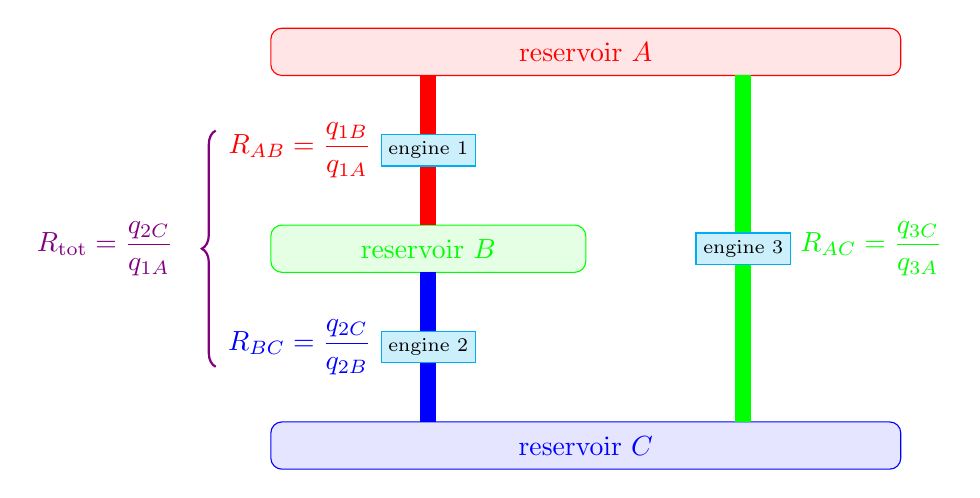
\begin{tikzpicture}
            \draw[blue,fill=blue!10,rounded corners] (0,0) rectangle (8,0.6);
            \node[blue] at (4,0.3) {reservoir \(C\)};

            \draw[green,fill=green!10,rounded corners] (0,2.5) rectangle (4,3.1);
            \node[green] at (2,2.8) {reservoir \(B\)};

            \draw[red,fill=red!10,rounded corners] (0,5) rectangle (8,5.6);
            \node[red] at (4,5.3) {reservoir \(A\)};

            \fill[red] (1.9,3.1) rectangle (2.1,5);
            \draw[cyan,fill=cyan!20] (1.4,3.85) rectangle (2.6,4.25);
            \node at (2,4.05) {\scriptsize engine 1};
            \node[red] at (1.4,4.05)[left]{\(\displaystyle R_{AB}=\frac{q_{1B}}{q_{1A}}\)};

            \fill[blue] (1.9,0.6) rectangle (2.1,2.5);
            \draw[cyan,fill=cyan!20] (1.4,1.35) rectangle (2.6,1.75);
            \node at (2,1.55) {\scriptsize engine 2};
            \node[blue] at (1.4,1.55)[left]{\(\displaystyle R_{BC}=\frac{q_{2C}}{q_{2B}}\)};

            \fill[green] (5.9,0.6) rectangle (6.1,5);
            \draw[cyan,fill=cyan!20] (5.4,2.6) rectangle (6.6,3);
            \node at (6,2.8) {\scriptsize engine 3};
            \node[green] at (6.6,2.8)[right]{\(\displaystyle R_{AC}=\frac{q_{3C}}{q_{3A}}\)};

            \draw [decorate,decoration={brace,amplitude=5pt,mirror},thick,violet] (-0.7,4.3) -- (-0.7,1.3) node[midway,xshift=-4 em]{\(\displaystyle R_{\text{tot}}=\frac{q_{2C}}{q_{1A}}\)};
        \end{tikzpicture}
    \end{figure}

    \subsubsection{Entropy}
    The reason we derived everything above is to introduce the entropy. To do so, we rewrite (\ref{absolute_temperature}) as
    \begin{equation}\label{reversible_heat_temperature}
        \frac{q_A}{T_A}=\frac{q_B}{T_B}\,,
    \end{equation}
    where \(q_A\) is the heat that flows in reversibly at the high temperature \(T_A\), and \(q_B\) is the heat that flows out reversibly at the low temperature \(T_B\). We see therefore that, during a complete cycle, the difference between \(q_A/T_A\) and \(q_B/T_B\) is zero. Recall that, at the end of a cycle, the internal energy of the system has not changed. Now (\ref{reversible_heat_temperature}) tells us that there is also another quantity that we call \textit{entropy} and that we denote by \(S\) that is unchanged when we restore the system to its original state. In the language of thermodynamics, we call \(S\) a \textit{state function}. We do not know what \(S\) is, but we do know how to compute its change. In the above example, the change in \(S\) was given by \(\Delta S=(q_A/T_A)-(q_B/T_B)=0\). In general, the change in entropy of a system due to the reversible addition of an infinitesimal amount of heat \(\delta q_{\text{rev}}\) from a reservoir at temperature \(T\) is
    \begin{equation}\label{entropy}
        \delta S=\frac{\delta q_{\text{rev}}}{T}\,.
    \end{equation}
    We also note that \(S\) is \textit{extensive}. That means that the total entropy of two non-interacting systems is equal to the sum of the entropies of the individual systems. Consider a system with a fixed number of particles \(N\) and a fixed volume \(V\). If we transfer an infinitesimal amount of heat \(\delta q\) to this system, then the change in the internal energy of the system, \(\d{E}\), is equal to \(\delta q\). Therefore
    \begin{equation}
        \left(\pdv{S}{E}\right)_{V,N}=\frac{1}{T}\,.
    \end{equation}

    From these, we can get the most famous, albeit not most intuitively obvious, statement of the second law of thermodynamics:
    \begin{law}[Second law of thermodynamics]
        Any spontaneous change in a system that exchanges neither heat nor particles with its environment can never lead to a decrease of the entropy.
    \end{law}
    Hence, at equilibrium, the entropy of an isolated system is at a maximum.

    \begin{figure}
        \centering
        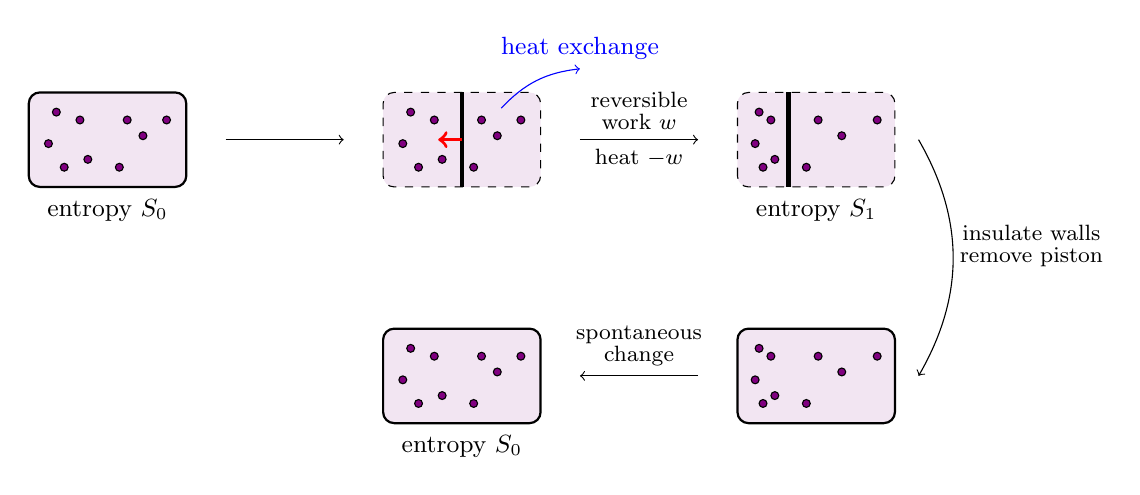
\begin{tikzpicture}
            \draw[fill=violet!10,rounded corners,thick] (0,0) rectangle (2,1.2);
            \node at (1,0.6) {\tikz{
                \draw[fill=violet] (0.5,0.3) circle (0.05);
                \draw[fill=violet] (0.3,0.6) circle (0.05);
                \draw[fill=violet] (0.4,1) circle (0.05);
                \draw[fill=violet] (1.2,0.3) circle (0.05);
                \draw[fill=violet] (1.3,0.9) circle (0.05);
                \draw[fill=violet] (0.8,0.4) circle (0.05);
                \draw[fill=violet] (1.5,0.7) circle (0.05);
                \draw[fill=violet] (1.8,0.9) circle (0.05);
                \draw[fill=violet] (0.7,0.9) circle (0.05);
            }};
            \node at (1,-0.3) {\small entropy \(S_0\)};
            \draw[->] (2.5,0.6)--(4,0.6);
            \draw[fill=violet!10,rounded corners,dashed] (4.5,0) rectangle (6.5,1.2);
            \node at (5.5,0.6) {\tikz{
                \draw[fill=violet] (0.5,0.3) circle (0.05);
                \draw[fill=violet] (0.3,0.6) circle (0.05);
                \draw[fill=violet] (0.4,1) circle (0.05);
                \draw[fill=violet] (1.2,0.3) circle (0.05);
                \draw[fill=violet] (1.3,0.9) circle (0.05);
                \draw[fill=violet] (0.8,0.4) circle (0.05);
                \draw[fill=violet] (1.5,0.7) circle (0.05);
                \draw[fill=violet] (1.8,0.9) circle (0.05);
                \draw[fill=violet] (0.7,0.9) circle (0.05);
            }};
            \draw[very thick] (5.5,0)--(5.5,1.2);
            \draw[->,blue] (6,1) to[bend left=20] (7,1.5)node[above]{\small heat exchange};
            \draw[very thick, red, ->] (5.5,0.6)--(5.2,0.6);
            \draw[->] (7,0.6)--node[above,align=center]{\footnotesize reversible \\[-4pt] \footnotesize work \(w\)}node[below]{\footnotesize heat \(-w\)}(8.5,0.6);

            \draw[fill=violet!10,rounded corners,dashed] (9,0) rectangle (11,1.2);
            \node at (10,0.6) {\tikz{
                \draw[fill=violet] (0.25,0.3) circle (0.05);
                \draw[fill=violet] (0.15,0.6) circle (0.05);
                \draw[fill=violet] (0.2,1) circle (0.05);
                \draw[fill=violet] (0.8,0.3) circle (0.05);
                \draw[fill=violet] (0.95,0.9) circle (0.05);
                \draw[fill=violet] (0.4,0.4) circle (0.05);
                \draw[fill=violet] (1.25,0.7) circle (0.05);
                \draw[fill=violet] (1.7,0.9) circle (0.05);
                \draw[fill=violet] (0.35,0.9) circle (0.05);
            }};
            \draw[ultra thick] (9.65,0)--(9.65,1.2);
            \node at (10,-0.3) {\small entropy \(S_1\)};

            \draw[->] (11.3,0.6) to[bend left=30] (11.3,-2.4);
            \node at (11.7,-0.75)[right,align=center]{\footnotesize insulate walls \\[-4pt] \footnotesize remove piston};

            \draw[fill=violet!10,rounded corners,thick] (9,-3) rectangle (11,-1.8);
            \node at (10,-2.4) {\tikz{
                \draw[fill=violet] (0.25,0.3) circle (0.05);
                \draw[fill=violet] (0.15,0.6) circle (0.05);
                \draw[fill=violet] (0.2,1) circle (0.05);
                \draw[fill=violet] (0.8,0.3) circle (0.05);
                \draw[fill=violet] (0.95,0.9) circle (0.05);
                \draw[fill=violet] (0.4,0.4) circle (0.05);
                \draw[fill=violet] (1.25,0.7) circle (0.05);
                \draw[fill=violet] (1.7,0.9) circle (0.05);
                \draw[fill=violet] (0.35,0.9) circle (0.05);
            }};

            \draw[fill=violet!10,rounded corners,thick] (4.5,-3) rectangle (6.5,-1.8);
            \node at (5.5,-2.4) {\tikz{
                \draw[fill=violet] (0.5,0.3) circle (0.05);
                \draw[fill=violet] (0.3,0.6) circle (0.05);
                \draw[fill=violet] (0.4,1) circle (0.05);
                \draw[fill=violet] (1.2,0.3) circle (0.05);
                \draw[fill=violet] (1.3,0.9) circle (0.05);
                \draw[fill=violet] (0.8,0.4) circle (0.05);
                \draw[fill=violet] (1.5,0.7) circle (0.05);
                \draw[fill=violet] (1.8,0.9) circle (0.05);
                \draw[fill=violet] (0.7,0.9) circle (0.05);
            }};
            \draw[->] (8.5,-2.4)--node[above,align=center]{\footnotesize spontaneous \\[-4pt] \footnotesize change}(7,-2.4);
            \node at (5.5,-3.3) {\small entropy \(S_0\)};
        \end{tikzpicture}
        \caption{To drive a system away from equilibrium, e.g. by changing the density, we need to do work. If we do this work reversibly and maintain the total energy of the system, this entails a loss of heat from the system. Hence \(S_1<S_0\). When we remove the constraint, the system spontaneously returns to equilibrium and its entropy is once again \(S_0\). For spontaneous changes, \(\Delta S>0\).}
    \end{figure}
    
    As an example, let us consider a system with an energy \(E\), volume \(V\) and number of particles \(N\) that is at equilibrium. The entropy of this system is \(S_0(E,V,N)\). Suppose we wish to change something in this system; for instance, we increase the density in one half and decrease it in the other. As the system was at equilibrium, this change does not occur spontaneously; in order to effect this change, we must perform a certain amount of work \(w\), for instance by placing a piston in the system and moving it. Let us perform this work reversibly in such a way that \(E\), the total energy of the system, stays constant, as do \(V\) and \(N\). The first law tells us that we can only keep \(E\) constant if, while we do the work, we allow an amount of heat \(q\) to flow out of the system, such that \(-q=w\). However, when an amount of heat \(-q\) flows out of the system, (\ref{entropy}) tells us that the entropy \(S\) of the system must decrease: \(S_1(E,V,N)<S_0(E,V,N)\).
    
    Having completed the change in the system, we insulate the system thermally from the rest of the world, and we remove the constraint that kept the system in its special constrained state. In our piston example, this might entail making a hole in the piston separating the two parts of the system. Now the system goes back spontaneously and irreversibly to equilibrium. However, since the volume is fixed, no work is done, and since the system is thermally insulated, no heat is transferred. Hence the final energy \(E\) is equal to the original energy, and \(V\) and \(N\) are also unchanged. This means that the system is now back in its original equilibrium state and its entropy is once more equal to \(S_0(E,V,N)\).

    The entropy change during this spontaneous change is equal to \(\Delta S=S_0-S_1\). But, as \(S_1<S_0\), it follows that \(\Delta S > 0\).

    \subsection{The Third Law}
    From this point on, we can derive all of thermodynamics, except one law --- the so-called third law of thermodynamics.
    \begin{law}[Third law of thermodynamics]
        At \(T=0\), the entropy of the equilibrium state of a pure, perfectly crystalline substance equals zero.
    \end{law}
    The third law is not nearly as fundamental as the first two, and in any case, as discussed in the main text, statistical mechanics gives us a more direct interpretation of its meaning.

    \subsection{Fundamental Equations}
    From the first law of thermodynamics, we write, in infinitesimal form
    \begin{equation}
        \d{E}_{\text{rev}}=\dbar q_{\text{rev}}+\dbar w_{\text{rev}}\,.
    \end{equation}
    If the system only does reversible \(PV\) work, then \(\dbar w_{\text{rev}}=-P\d{V}\). For reversible processes, the \textit{Clausius inequality}, \(\d{S}\ge\dbar q/T\) is an equality (\ref{entropy}); this is a statement of the second law of thermodynamics. Thus we can write \(\d{E}_{\text{rev}}=T\d{S}-P\d{V}\). Since the internal energy is a state function, this equation applies between any equilibrium state, not just along reversible pathways. The equation is known as the \textit{fundamental equation} for the internal energy.

    \subsubsection{Legendre Transforms}
    Consider a general function \(f(x,y)\), whose total differential is
    \begin{equation}
        \d{f}=\left(\pdv{f}{x}\right)_y\d{x}+\left(\pdv{f}{y}\right)_x\d{y}=u\d{x}+v\d{y}\,.
    \end{equation}
    Since \(u\) is the derivative of \(f\) with respect to \(x\), we say that \(u\) and \(x\) are \textit{conjugate variables}. Then, consider the function \(F=f-(ux)\), whose differential is
    \begin{equation}
        \d{F}=\d{f}-\d{(ux)}=v\d{y}-x\d{u}\,.
    \end{equation}
    The function \(F\) is known as the \textit{Legendre transform} of \(f\). Evidently, \(F\) remains a function of \(y\), but is now a function of \(u\), the conjugate pair of \(x\), rather than of \(x\) itself.

    To see how this formalism can be applied to thermodynamics, consider the \textit{enthalpy}. When you were first introduced to it in Part IA, we said that we wanted a state function corresponding to the heat flow at constant pressure. But how do we know how to define it? The enthalpy is the appropriate measure of ``energy'' for a system at constant pressure rather than constant volume, so we would like to convert \(E=E(S,V)\) into \(H=H(S, P)\) so that \(P\) is a natural variable of our function \(H\) that we can control, and \(V\) is a derived property. The enthalpy is the Legendre transform of \(E\), defined as
    \begin{equation}
        H=E+PV
    \end{equation}
    so that
    \begin{equation}
        \d{H}=T\d{S}+V\d{P}\,.
    \end{equation}
    Similarly, we may change the natural variable from \(S\) to \(T\) for internal energy and enthalpy, giving \textit{Helmholtz free energy} \(A=A(T,V)\) and \textit{Gibbs free energy} \(G=G(T,P)\) defined by Legendre transforms
    \begin{align}
        A&=E-TS\,,\\
        G&=H-TS\,,
    \end{align}
    so that we have the fundamental equations
    \begin{align}
        \d{A}&=-S\d{T}-P\d{V}\\
        \d{G}&=-S\d{T}+V\d{P}\,.
    \end{align}

    The above relations are for the cases where the number of particles \(N\) is fixed. If the number of particles can also change, we need to add a further term \(+\mu\d{N}\) to the above fundamental equations, where \(\mu\) is the \textit{chemical potential}. This allows us to define further Legendre transforms to change the natural variables from \(N\) to \(\mu\). The one we are interested in is the \textit{Grand potential}
    \begin{equation}
        \Phi=E-TS-N\mu\,,
    \end{equation}
    so that
    \begin{equation}
        \d{\Phi}=-S\d{T}-P\d{V}-N\d{\mu}\,.
    \end{equation}

    This completes the definition of the five most common \textit{thermodynamic potentials}: \(E,H,A,G,\Phi\). More thermodynamic potentials can be defined by doing further Legendre transforms, but they are of less interest.

    \subsubsection{Maxwell Relations}
    Schwarz's theorem guarantees that if \(f=f(x,y,\dots)\) have continuous second partial derivatives, then
    \begin{equation}
        \pdv{}{x}\left(\pdv{f}{y}\right)=\pdv{}{y}\left(\pdv{f}{x}\right)\,.
    \end{equation}
    Since the fundamental equations are exact differentials, we can apply the Schwarz's theorem to our thermodynamic potentials. For example, from the fundamental equation of the internal energy
    \begin{equation}
        \d{E}=T\d{S}-P\d{V}+\mu\d{N}\,,
    \end{equation}
    we have
    \begin{equation}
        \left[\pdv{}{V}\left(\pdv{E}{S}\right)_V\right]_{S}=\left[\pdv{}{S}\left(\pdv{E}{V}\right)_S\right]_{V}\,,
    \end{equation}
    which gives the relation
    \begin{equation}
        \left(\pdv{T}{V}\right)_{S}=-\left(\pdv{P}{S}\right)_{V}\,.
    \end{equation}
    We can get a lot more relations like this from the fundamental equations of different thermodynamic potentials, using the symmetry of partial derivatives with respect to different variables. They are called the \textit{Maxwell relations}. They are not worth memorising as they can be easily derived.

    \subsubsection{Euler Relations}
    Since all natural variables of the internal energy \(E\) are extensive quantities,
    \begin{equation}
        \alpha E(N,V,S)=E(\alpha N, \alpha V, \alpha S)
    \end{equation}
    for \(\alpha\in\mathbb{R}\). The total differential is now
    \begin{equation}
        \d{(\alpha E)}=\left(\pdv{(\alpha E)}{(\alpha N)}\right)_{\alpha V,\alpha S}\d{(\alpha N)}+\left(\pdv{(\alpha E)}{(\alpha V)}\right)_{\alpha N,\alpha S}\d{(\alpha V)}+\left(\pdv{(\alpha E)}{(\alpha S)}\right)_{\alpha N, \alpha V}\d{(\alpha S)}\,.
    \end{equation}
    Differentiating both sides with respect to \(\alpha\) gives
    \begin{align}
        \left(\pdv{(\alpha E)}{\alpha}\right)_{N,V,S}&=\left(\pdv{(\alpha E)}{(\alpha N)}\right)_{\alpha V,\alpha S}\left(\pdv{(\alpha N)}{\alpha}\right)_{N,V,S}\notag\\
        &\quad +\left(\pdv{(\alpha E)}{(\alpha V)}\right)_{\alpha N,\alpha S}\left(\pdv{(\alpha V)}{\alpha}\right)_{N,V,S}\notag\\
        &\quad +\left(\pdv{(\alpha E)}{(\alpha S)}\right)_{\alpha N, \alpha V}\left(\pdv{(\alpha S)}{\alpha}\right)_{N,V,S}\,.
    \end{align}
    Simplify this derivative and set \(\alpha=1\) gives
    \begin{align}
        E&=\left(\pdv{E}{N}\right)_{V,S}N+\left(\pdv{E}{V}\right)_{N,S}V+\left(\pdv{E}{S}\right)_{N,V}S\notag\\
        &=\mu N-PV+TS\,.
    \end{align}
    This is the \textit{Euler relation}.\footnote{It was not discovered by Euler in an investigation of thermodynamics, which did not exist in his day. It is called the Euler relation just because Euler's theorem on homogeneous functions leads to it.}

    Substituting the Euler relation into the expressions for the other main potentials gives
    \begin{align}
        A&=-PV+\mu N\\
        H&=TS+\mu N\\
        G&=\mu N\\
        \Phi&=-PV\,.
    \end{align}
    This is essentially why we said the chemical potential \(\mu\) is equal to the Gibbs energy per particle.

    We may differentiate \(G=\mu N\) to get \(\d{G}=N\d{\mu}+\mu\d{N}\). From the fundamental equation \(\d{G}=-S\d{T}+V\d{P}+\mu\d{N}\), we can get the \textit{Gibbs--Duhem relation}
    \begin{equation}
        N\d{\mu}=V\d{P}-S\d{T}\,.
    \end{equation}

    \section{From Quantum to Classical}\label{Chap:Quantum_to_Classical}
    It is possible to derive the classical partition function directly from the quantum partition function without resorting to hand-waving. It will also show us why the factor of \(1/h\) sits outside the partition function. The derivation is a little tedious, but worth seeing. (Similar techniques are useful in later courses when you first meet the path integral). To make life easier, let's consider a single particle moving in one spatial dimension. It has position operator \(\hat{x}\), momentum operator \(\hat{p}\) and Hamiltonian
    \begin{equation}
        \hat{H}=\frac{\hat{p}^2}{2m}+V(\hat{x})\,.
    \end{equation}
    If \(\ket{n}\) is the energy eigenstate with energy \(E_n\), the quantum partition function is
    \begin{equation}
        Q=\sum_n \ee^{-\beta E_n}=\sum_n\expval{\ee^{-\beta\hat{H}}}{n}\,,
    \end{equation}
    where the exponential of an operator \(\hat{X}\) is defined via the expansion
    \begin{equation}
        \ee^{\hat{X}}=\sum_{n=0}^{\infty}\frac{\hat{X}^n}{n!}\,.
    \end{equation}
    In what follows, we'll make liberal use of the fact that we can insert the identity operator anywhere in this expression. We have the resolution of the identities in the position eigenstates \(\ket{x}\) and the momentum eigenstates \(\ket{p}\):
    \begin{equation}
        1=\int\dd{x}\ket{x}\bra{x} \text{ and } 1=\int\dd{p}\ket{p}\bra{p}\,.
    \end{equation}
    We insert two copies of the identity built from position eigenstates into our partition function to get
    \begin{align}
        Q&=\sum_n\mel{n}{\int\dd{x}}{x}\mel{x}{\ee^{-\beta\hat{H}}\int\dd{x'}}{x'}\braket{x'}{n}\notag \\
        &=\int\dd{x}\dd{x'}\mel{x}{\ee^{-\beta\hat{H}}}{x'}\sum_n\braket{x'}{n}\braket{n}{x}\,.
    \end{align}
    And now \(\sum_n\ket{n}\bra{n}\) is the identity, while \(\ket{x'}\bra{x}=\delta(x-x')\), so
    \begin{equation}
        Q=\int\dd{x}\expval{\ee^{-\beta\hat{H}}}{x}\,.
    \end{equation}
    We see that the result is to replace the sum over energy eigenstates with a sum (or integral) over position eigenstates. If you wanted, you could play the same game and get the sum over any complete basis of eigenstates of your choosing. This means that we can write the partition function in a basis independent fashion as
    \begin{equation}
        Q=\tr \ee^{-\beta\hat{H}}\,.
    \end{equation}

    So far, our manipulations could have been done for any quantum system. Now we want to use the fact that we are taking the classical limit. This comes about when we try to factorize \(\ee^{-\beta H}\) into a momentum term and a position term --- the trouble is that this isn't always possible when there are matrices (or operators) in the exponent. The Hamiltonian \(\hat{H}\) is the sum of a kinetic part \(\hat{T}\) and a potential part \(\hat{V}\).  The kinetic energy eigenstates are also the momentum eigenstates, but potential energy eigenstates are the position eigenstates, so \(\hat{H}=\hat{T}+\hat{V}\) is not diagonal in either basis i.e. \(\hat{T}\) and \(\hat{V}\) does not commute. In fact, we have
    \begin{equation}
        \ee^{\hat{A}}\ee^{\hat{B}}=\ee^{\hat{A}+\hat{B}+\frac{1}{2}[\hat{A},\hat{B}]+\dots}\,.
    \end{equation}
    For us \([x,p]=i\hbar\). This means that if we're willing to neglect terms of order \(\hbar\) --- which is the meaning of taking the classical limit --- then we can write
    \begin{equation}
        \ee^{-\beta\hat{H}}=\ee^{-\beta \hat{T}}\ee^{-\beta \hat{V}}=\ee^{-\beta\hat{p}^2/2m}\ee^{-\beta V(\hat{x})}\,.
    \end{equation}
    We can now start to replace some of the operators in the exponent, like \(V(\hat{x})\), with functions \(V(x)\). (Note the subtle but important notational difference!)
    \begin{align}
        Q&=\int\dd{x}\expval{\ee^{-\beta V(\hat{x})}\ee^{-\beta\hat{p}^2/2m}}{x}\notag\\
        &=\int\dd{x}\dd{x'}\dd{r}\dd{r'}\mel{x}{\ee^{-\beta\hat{V}(\hat{x})}}{x'}\braket{x'}{p}\mel{p}{\ee^{-\beta\hat{p}^2/2m}}{p'}\braket{p'}{x}\notag \\
        &=\int\dd{x}\dd{p}\mel{x}{\ee^{-\beta\hat{V}(\hat{x})}}{x}\braket{x}{p}\mel{p}{\ee^{-\beta\hat{p}^2/2m}}{p}\braket{p}{x}\notag \\
        &=\int\dd{x}\dd{p}\abs{\braket{x}{p}}^2 \ee^{-\beta p^2/2m}\ee^{-\beta V(x)}\,,
    \end{align}
    where we have used the fact that all matrix elements are diagonal. We have that
    \begin{equation}
        \braket{x}{p}=\frac{1}{\sqrt{2\pi\hbar}}\ee^{\ii px/\hbar}
    \end{equation}
    is the wavefunction of the momentum eigenstate, so
    \begin{equation}
        Q=\frac{1}{h}\int\dd{x}\dd{p}\ee^{-\beta H(x,p)}\,.
    \end{equation}

    \section{Pressure from Clausius Virial}
    Very often, there is not just one way of deriving a particular result. In the main text, we derived an expression for the pressure of interacting particles in terms of the inter-particle forces directly from the partition function by using a scaling argument. We show here a derivation using a completely different line of reasoning, originally proposed by Clausius.

    Consider a system of \(N\) particles in a volume \(V\) at total energy \(E\). Define the \textit{virial} of the system to be
    \begin{equation}
        \mathcal{V}\coloneqq\sum_{i=1}^{N}\vb{r}_i\vdot\vb{p}_i\,.
    \end{equation}
    This is one half of the time derivative of the moment of inertia \(I\) of the system since
    \begin{equation}
        \frac{1}{2}\pdv{I}{t}=\frac{1}{2}\sum_{i=1}^{N}m_i\pdv{}{t}\vb{r}_i\vdot\vb{r}_i=\sum_{i=1}^{N}m_i\vb{r}_i\vdot\dot{\vb{r}}_i=\mathcal{V}\,.
    \end{equation}
    Since the particles are constrained in a container, and the total kinetic energy is bounded by \(E\), \(\mathcal{V}\) is also bounded both above and below, by \(\mathcal{V}_{\text{max}}\) and \(\mathcal{V}_{\text{min}}\). At long times \(\tau\to\infty\), the time average of the time derivative of \(\mathcal{V}\), denoted by \(\dot{\mathcal{V}}\), vanishes:
    \begin{equation}
        \overline{\dot{\mathcal{V}}}=\frac{1}{\tau}\int_{0}^{\tau}\dot{\mathcal{V}}(t)\dd{t}=\frac{\mathcal{V}(\tau)-\mathcal{V}(0)}{\tau}\to 0\text{ as }\tau\to\infty\,.
    \end{equation}

    We can also evaluate this time derivative explicitly:
    \begin{equation}
        \overline{\dot{\mathcal{V}}}=\sum_{i=1}^{N}\overline{\dot{\vb{r}}_i\vdot\vb{p}_i}+\overline{\vb{r}_i\vdot\dot{\vb{p}}_i}=0\,.
    \end{equation}
    We have \(\dot{\vb{r}}_i=\vb{p}_i/m_i\) and \(\dot{\vb{p}}_i=\vb{f}_i\) by Newton's second law, where \(\vb{f}_i\) is the force on the particle \(i\), so we can write
    \begin{equation}
        \sum_{i=1}^{N}\frac{\overline{p_i^2}}{m_i}+\overline{\vb{r}_i\vdot\vb{f}_i}=0\,.
    \end{equation}
    The first term on the left is simply twice the kinetic energy of the system. Using the equipartition theorem, we can write this as \(3Nk_BT\). We thus find that
    \begin{equation}
        3Nk_B T+\sum_{i=1}^{N}\overline{\vb{r}_i\vdot\vb{f}_i}=0\,.
    \end{equation}

    The force \(\vb{f}_i\) acting on a particle can originate either from the intermolecular interactions or interactions with the wall of the container. Let us consider the contribution to the virial due to the interaction with a surface element \(\d{\vb{S}}\) of the wall of the container. We denote the position of this surface element by \(\vb{r}_S\). Whenever a particle collides with this surface element, its coordinate must be given by \(\vb{r}_S\). The contribution to the force virial arising from collisions with this surface element is thus given by
    \begin{equation}
        \overline{\left(\sum_{i=1}^{N}\vb{r}_i\vdot\vb{f}_i\right)^{(\d{\vb{S}})}}=\sum_{i=1}^{N}\overline{\vb{r}_S\vdot\vb{f}_i^{(\d{\vb{S}})}}=\vb{r}_S\vdot\sum_{i=1}^{N}\overline{\vb{f}_i^{(\d{\vb{S}})}}=\vb{r}_S\vdot\overline{\vb{F}_\text{tot}^{\d{\vb{S}}}}\,.
    \end{equation}
    \(\overline{\vb{F}_\text{tot}^{\d{\vb{S}}}}\) is the average total force exerted on the particles by the wall of the container --- by Newton's third law, this is also the force exerted on the container wall by the particles. This is exactly the force causing the pressure! Therefore we have
    \begin{equation}
        \overline{\left(\sum_{i=1}^{N}\vb{r}_i\vdot\vb{f}_i\right)^{(\d{\vb{S}})}}=\vb{r}_S\vdot(-P)\d{\vb{S}}\,.
    \end{equation}
    We can now integrate over the entire surface of the container to obtain
    \begin{equation}
        \sum_{i=1}^{N}\overline{\vb{r}_i\vdot\vb{f}_i}=-P\int\dd{\vb{S}}\vdot\vb{r}_S\,.
    \end{equation}
    Using the divergence theorem, we can write
    \begin{equation}
        -P\int\dd{\vb{S}}\vdot\vb{r}_S=-P\int\dd{V}(\div\vb{r})=-3PV\,.
    \end{equation}
    Therefore,
    \begin{equation}
        3Nk_B T+\sum_{i=1}^{N}\overline{\vb{r}_i\vdot\vb{f}_i^{\text{inter}}}-3PV=0\,.
    \end{equation}
    We get the same result
    \begin{equation}
        P=\frac{Nk_B T}{V}+\frac{1}{3V}\eval{\sum_{i=1}^{N}\vb{r}_i\vdot\vb{f}_i}\,,
    \end{equation}
    where notice that we have replaced the time average by a Boltzmann-weighted average over states at constant \(N\), \(V\) and \(T\).

    \section{Ising and Lattice-Gas Model Equivalence}\label{Chap:Ising_Lattice_Gas}
    The Ising model for a lattice of interacting magnetic spins is amongst the most widely used models in physics because many other models can be mapped onto it. As an example, we consider the relation between the Ising model and a lattice gas. The lattice gas model is a simple model used to describe the liquid-vapour transition. Let us first consider the Ising model, in which neighbouring parallel spins have an interaction energy \(-J\), whilst anti-parallel spins have an interaction energy \(+J\). We denote the value of the spin on lattice site \(i\) by \(s_i\in\{\pm 1\}\). The Ising Hamiltonian in the presence of a magnetic field \(B\) is given by
    \begin{equation}
        H_{\text{Ising}}=-\frac{J}{2}\sum_{i=1}^{N}\sum_{\langle i,j\rangle}s_is_j-B\sum_{i=1}^{N}s_i\,.
    \end{equation}
    The partition function of the Ising model can be written as
    \begin{equation}\label{Q_ising}
        Q_{\text{Ising}}=\sum_{(s_k)_{k=1}^{N}}\exp\left[-\beta\left(-\frac{J}{2}\sum_{i=1}^{N}\sum_{\langle i,j\rangle}s_is_j-B\sum_{i=1}^{N}s_i\right)\right]\,,
    \end{equation}
    where \((s_k)_{k=1}^{N}\) denote all possible arrangements of spin values \((s_1,\dots,s_N)\).

    Now consider a gas on a lattice with \(N\) sites, where there can be at most one particle per lattice site. Neighbouring particles have an interaction energy \(-\epsilon\). The Hamiltonian is
    \begin{equation}
        H_{\text{LG}}=-\frac{\epsilon}{2}\sum_{i=1}^{N}\sum_{\langle i,j\rangle}n_in_j\,,
    \end{equation}
    where \(n_i\in\{0,1\}\) denotes the number of particles on site \(i\). The partition function is
    \begin{equation}
        Q_{\text{LG}}(M)=\sum_{(n_k)_{k=1}^{N}|_M}\exp\left[-\beta\left(-\frac{\epsilon}{2}\sum_{i=1}^{N}\sum_{\langle i,j\rangle}n_in_j\right)\right]\,,
    \end{equation}
    where \(M\) is the number of particles and \((n_k)_{k=1}^{N}|_M\) is the arrangement of occupation numbers that satisfy \(\sum_i n_i=M\). It turns out to be more convenient to consider the grand partition function \(\Xi\) instead to remove this awkward constraint.
    \begin{align}
        \Xi&=\sum_{M=0}^{N}\sum_{(n_k)_{k=1}^{N}|_M}\exp\left[-\beta\left(-\frac{\epsilon}{2}\sum_{i=1}^{N}\sum_{\langle i,j\rangle}n_in_j\right)\right]\ee^{\beta\mu M} \notag \\
        &=\sum_{(n_k)_{k=1}^{N}}\exp\left[-\beta\left(-\frac{\epsilon}{2}\sum_{i=1}^{N}\sum_{\langle i,j\rangle}n_in_j-\mu\sum_{i=1}^{N}n_i\right)\right]\,. \label{Xi_lattice_gas}
    \end{align}
    This looks remarkably similar to the canonical partition function of the Ising model (\ref{Q_ising}) --- it seems that we only need to change the letters and (\ref{Xi_lattice_gas}) will become (\ref{Q_ising}). But there is actually an important difference: \(s_i\) takes value in \(\{\pm 1\}\), while \(n_i\) takes value in \(\{0,+1\}\). We have to identify \(s=2n-1\) to make the exact mapping between the two cases. On doing so, we also need to identify
    \begin{equation}
        J=\frac{\epsilon}{4} \text{ and }B=\frac{\mu}{2}+\frac{q\epsilon}{4}\,.
    \end{equation}
    After doing so, the grand partition function of this lattice gas will be exactly the same as the canonical partition function of an Ising model in a magnetic field. This probably makes the universality we introduced in the main text less shocking than it first seems.

    \section{More on Interacting Gases}\label{Chap:Cluster_Expansion}
    In this section, we will re-do some of our previous calculations in a more unified approach, and extend the results to the beautiful and important cluster expansions.\footnote{This section is extremely mathematically demanding. This is included in my notes because of my personal interests. This is not in the official notes.}
    \subsection{Mayer \texorpdfstring{\(\bm{f}\)}{f} Functions and Second Virial Coefficients}
    The Hamiltonian of the interacting gas is
    \begin{equation}
        H=\sum_{i=1}^{N}\frac{p_i^2}{2m}+\sum_{i>j}U(r_{ij})\,.
    \end{equation}
    We would like to find a general method calculating the coefficients for the \textit{virial expansion}
    \begin{equation}
        \frac{p}{k_B T}=\frac{N}{V}+B_2(T)\frac{N^2}{V^2}+B_3(T)\frac{N^3}{V^3}+\dots
    \end{equation}
    As we've seen before, the partition function is
    \begin{align}
        Q(N,V,T)&=\frac{1}{h^{3N}N!}\int\prod_{i=1}^{N}\dd[3]{\vb{p}_i}\dd[3]{\vb{r}_i}\ee^{-\beta H}\notag\\
        &=\frac{1}{\Lambda^{3N}N!}\int\prod_{i}\dd[3]{\vb{r}_i}\ee^{-\beta\sum_{j<k}U(r_{jk})}\,.
    \end{align}
    We still need to do the integral over positions, which looks hard. The interactions mean that the integrals don't factor in any obvious way.

    An obvious thing to try is the Taylor expansion, which should better be called a \textit{cumulant expansion} in this context.
    \begin{equation}
        \ee^{-\beta\sum_{j<k}U(r_{jk})}=1-\beta\sum_{j<k}U(r_{jk})+\frac{\beta^2}{2}\sum_{j<k,l<m}U(r_{jk})U(r_{lm})+\dots
    \end{equation}
    Unfortunately, this is not very useful. We want each term to be smaller than the preceding one. But as \(r_{ij}\to 0\), the potential \(U(r_{ij})\to\infty\), which does not look promising for an expansion parameter.

    We will instead work with the following quantity called the \textit{Mayer \(f\) function}.
    \begin{equation}
        f(r)\coloneqq \ee^{-\beta U(r)}-1\,.
    \end{equation}
    This is a nicer expansion parameter. When the particles are far, \(f(r)\to 0\) and when particles are close, \(f(r)\to -1\).

    Let us define
    \begin{equation}
        f_{ij}=f(r_{ij})\,,
    \end{equation}
    then we can write the partition function as
    \begin{align}
        Q(N,V,T)&=\frac{1}{\Lambda^{3N}N!}\int\prod_{i}\dd[3]{\vb{r}_i}\prod_{j>k}(1+f_{jk})\notag\\
        &=\frac{1}{\Lambda^{3N}N!}\int\prod_{i}\dd[3]{\vb{r}_i}\left(1+\sum_{j>k}f_{jk}+\sum_{j>k,l>m}f_{jk}f_{lm}+\dots\right)\,.
    \end{align}
    The first term simply gives a factor of the volume \(V\) for each integral, so we get \(V^N\). The second term has a sum, each element of which is the same. They all look like
    \begin{equation}
        \int\prod_{i=1}^{N}\dd[3]{\vb{r}_i}f_{12}=V^{N-2}\int\dd[3]{\vb{r}_1}\dd[3]{\vb{r}_2}f(r_{12})=V^{N-1}\int\dd[3]{\vb{r}}f(r)\,,
    \end{equation}
    where, in the last equality, we have changed the integration variables from \(\vb{r}_1\) and \(\vb{r}_2\) to the centre of mass \(\vb{R}=\frac{1}{2}(\vb{r}_1+\vb{r}_2)\) and the separation \(\vb{r}=\vb{r}_1-\vb{r}_2\). You might worry that the limits of integration change in the integral over \(\vb{r}\), but the integral over \(f(r)\) only picks up contributions from atomic size distances and this is only actually a problem close to the boundaries of the system where it is negligible.

    There is a term like this for each pair of particles, so there are in total \(\frac{1}{2}N(N-1)\approx\frac{1}{2}N^2\) terms. Then ignoring terms \(O(f^2)\), the partition function is given approximately by
    \begin{align}
        Q(N,V,T)&=\frac{V^N}{\Lambda^{3N}N!}\left(1+\frac{N^2}{2V}\int\dd[3]{\vb{r}}f(r)+\dots\right)\notag\\
        &=Q_{\text{ideal}}\left(1+\frac{N}{2V}\int\dd[3]{\vb{r}}f(r)+\dots\right)^N\,,
    \end{align}
    where we promoted one power of \(N\) from the front of the integral to an overall exponent. Massaging the expression in this way ensures that the free energy is proportional to the number of particles as one would expect:
    \begin{equation}\label{intgasf}
        A=-k_BT\ln Q=A_\text{ideal}-Nk_BT\ln\left(1+\frac{N}{2V}\int\dd[3]{\vb{r}}f(r)\right)\,.
    \end{equation}
    From this expression for the free energy, it is clear that we are indeed performing an expansion in density of the gas since the correction term is proportional to \(N/V\). This form of the free energy will give us the second virial coefficient \(B_2(T)\).

    We can be somewhat more precise about what it means to be at low density in which our expression is valid. The exact form of the integral \(\int \dd[3]{\vb{r}}f(r)\) depends on the potential, but for both the Lennard Jones potential and the hard-core repulsion the integral is approximately \(\int\dd[3]{\vb{r}}f(r)\sim r_0^3\), where \(r_0\) some measure of the length scale of the potential (We will compute this later). For the expansion to be valid, we want each term with an extra power of \(f\) to be smaller than the preceding one. That means that the second term in the argument of the log should be smaller than \(1\). In other words,
    \begin{equation}
        \frac{N}{V}\ll\frac{1}{r_0^3}\,.
    \end{equation}
    We have a name for the substance packed as closely as in the right hand side --- we call them \textit{liquids}. Our expansion is valid for densities of the gas that are much lower than that of the liquid state.
    \subsection{van der Waals Equation of State}
    We can use the free energy \cref{intgasf} to compute the pressure of the gas. Expanding the log gives
    \begin{equation}
        P=-\pdv{A}{V}=\frac{Nk_BT}{V}\left(1-\frac{N}{2V}\int\dd[3]{\vb{r}}f(r)+\dots\right)\,.
    \end{equation}
    As expected, the pressure deviates from that of an ideal gas. We can characterise this by writing
    \begin{equation}\label{intgaseqstate}
        \frac{PV}{Nk_BT}=1-\frac{N}{2V}\int\dd[3]{\vb{r}}f(r)\,.
    \end{equation}
    To understand this, we need to calculate the integral. But first, let us look at two trivial examples.
    \begin{itemize}[topsep=0pt]
        \item Repulsion. Suppose that \(U(r)>0\) for all \(r\) with \(U(\infty)=0\). Then \(f<0\) and so the pressure will increase.
        \item Attraction. If \(U(r)<0\) then \(f>0\) and so the pressure will decrease.
    \end{itemize}

    Let's try this with some different potentials. We can define a hard core potential with van der Waals attraction
    \begin{equation}
        U(r)=\begin{cases}
            \infty & r< r_0 \\
            -U_0\left(\frac{r_0}{r}\right)^6 & r\ge r_0\,.
        \end{cases}
    \end{equation}
    The integral of the Mayer \(f\) function is
    \begin{equation}
        \int\dd[3]{\vb{r}}f(r)=\int_{0}^{r_0}\dd[3]\vb{r}(-1)+\int_{r_0}^{\infty}\dd[3]{\vb{r}}\left(\ee^{\beta U_0(r_0/r)^6}-1\right)\,.
    \end{equation}
    We will approximate the second integral in the high temperature limit with \(\beta U_0\ll 1\), where \(\ee^{\beta U_0(r_0/r)^6}\approx 1+\beta U_0(r_0/r)^6\). Then
    \begin{align}
        \int\dd[3]{\vb{r}}f(r)&=-4\pi\int_{0}^{r_0}\dd{r}r^2+\frac{4\pi U_0}{k_BT}\int_{r_0}^{\infty}\dd{r}\frac{r_0^6}{r^4}\notag\\
        &=\frac{4\pi r_0^3}{3}\left(\frac{U_0}{k_BT}-1\right)\,.
    \end{align}
    Insert this into \cref{intgaseqstate}, we have
    \begin{equation}
        \frac{PV}{Nk_BT}=1-\frac{N}{V}\left(\frac{a}{k_BT}-b\right)\,,
    \end{equation}
    where \(a\) and \(b\) are constants defined by
    \begin{equation}
        a=\frac{2\pi r_0^3 U_0}{3}\;\;,\quad b=\frac{2\pi r_0^3}{3}\,.
    \end{equation}
    We can recognise that this is indeed the second virial coefficient.

    We can rearrange this equation to a more useful form
    \begin{equation}
        k_BT=\frac{V}{N}\left(P+\frac{N^2}{V^2}a\right)\left(1+\frac{N}{V}b\right)^{-1}\,.
    \end{equation}
    As we are working in an expansion in density, we can do another Taylor expansion to get
    \begin{equation}\label{vanderwaals}
        k_BT=\left(P+\frac{N^2}{V^2}a\right)\left(\frac{V}{N}-b\right)\,.
    \end{equation}
    This again gives the famous van der Waals equation of state. This equation is valid at low densities and high temperatures.

    It seems that the equation we obtained (\ref{intgaseqstate}) can be used to compute the equation of state for any potential between atoms. However, there are limitations. The integral only converges for the long-range potentials in the form \(1/r^n\) when \(n\ge 4\). This means that the techniques described above do not work for long-range potentials with fall-off \(1/r^3\) or slower. This includes the important case of \(1/r\) Coulomb interactions.

    \subsection{The Cluster Expansion}
    We will now develop the full expansion and explain how to compute the higher virial coefficients.
    
    Let us go back to our first expression of the partition function in terms of \(f\).
    \begin{align}
            Q(N,V,T)&=\frac{1}{\Lambda^{3N}N!}\int\prod_{i}\dd[3]{\vb{r}_i}\prod_{j>k}(1+f_{jk})\notag\\
            &=\frac{1}{\Lambda^{3N}N!}\int\prod_{i}\dd[3]{\vb{r}_i}\left(1+\sum_{j>k}f_{jk}+\sum_{j>k,l>m}f_{jk}f_{lm}+\dots\right)\,. \label{intgaspf}
    \end{align}
    Above we effectively related the second virial coefficient to the term linear in \(f\): this is the essence of the equation of state \cref{intgaseqstate}. One might think that terms quadratic in \(f\) give rise to the third virial coefficient and so on. But we will see that the expansion is more subtle than that.

    The expansion in \cref{intgaspf} includes terms of the form \(f_{ij}f_{kl}f_{mn}\dots\), where the indices denote pairs of atoms, \((i,j)\) and \((k,l)\) and so on. These pairs may have atoms in common or they may all be different. However, the same pair never appears twice in a given term as you may check by going back to the first line in \cref{intgaspf}.
    
    We will introduce a diagrammatic method to keep track of all the terms in the sum. To each term of the form \(f_{ij}f_{kl}f_{mn}\dots\) we associate a picture using the following rules:
    \begin{itemize}[topsep=0pt]
        \item Draw \(N\) atoms (We actually need pictures with much less than \(N\sim 10^{23}\) atoms).
        \item Draw a line to connect each pair of atoms that appear as indices.
    \end{itemize}
    This allows us to never repeat the same pair of indices.

    For example, if \(N=4\), we may have the following pictures for different terms in the expansion:
    \begin{equation}\begin{aligned}
        f_{12}&=\tikz[baseline=1em]{
        \fourpoints
        \draw[thick] (0,0) -- (1,0);
    } & f_{12}f_{34}&=\tikz[baseline=1em]{
        \fourpoints
        \draw[thick] (0,0) -- (1,0);
        \draw[thick] (0,1) -- (1,1);
    }\\
    f_{12}f_{23}&=\tikz[baseline=1em]{
        \fourpoints
        \draw[thick] (0,0) -- (1,0);
        \draw[thick] (0,1) -- (1,0);
    } & f_{12}f_{23}f_{13}&=\tikz[baseline=1em]{
        \fourpoints
        \draw[thick] (0,0) -- (1,0);
        \draw[thick] (0,1) -- (1,0);
        \draw[thick] (0,0) -- (0,1);
    }\,.
    \end{aligned}\end{equation}
    We call these diagrams \textit{graphs}. Each possible graph appears exactly once in the partition function \cref{intgaspf}. In other words, the partition function is a sum over all graphs. We still have to do the integrals over all positions \(r_i\). We will denote the integral over graph \(G\) to be \(W[G]\). Then the partition function is
    \begin{equation}
        Q(N,V,T)=\frac{1}{\Lambda^{3N}N!}\sum_G W[G]\,.
    \end{equation}
    Nearly all the graphs that we can draw will have disconnected components. For example, those graphs that correspond to just a single \(f_{ij}\) will have two atoms connected and the remaining \(N-2\) sitting alone. Those graphs that correspond to \(f_{ij}f_{kl}\) fall into two categories: either they consist of two pairs of atoms (like the second example above) or, if \((i,j)\) shares an atom with \((k,l)\), there are three linked atoms (like the third example above). Importantly, the integral over positions \(\vb{r}_i\) then factorises into a product of integrals over the positions of atoms in disconnected components. This is illustrated by an example with \(N=5\) atoms
    \begin{equation}
        W\left[\tikz[baseline=1em]{
        \threepointslb
        \draw[thick] (0,0) -- (1,0);
        \draw[thick] (0,0) -- (0.5,1);
        \draw[thick] (1,0) -- (0.5,1)
    }\tikz[baseline=1em]{
        \draw[fill = black] (0,0) circle (0.05)node[left]{\small 4};
        \draw[fill = black] (0,1) circle (0.05)node[left]{\small 5};
        \draw[thick] (0,0) -- (0,1);
    }\;\;\right]=\left(\int\dd[3]{\vb{r}_1}\dd[3]{\vb{r}_2}\dd[3]{\vb{r}_3}f_{12}f_{23}f_{31}\right)\left(\int\dd[3]{\vb{r}_4}\dd[3]{\vb{r}_5}f_{45}\right)\,.
    \end{equation}
    We call the disconnected components of the graph \textit{clusters}. If a cluster has \(\ell\) atoms, we will call it an \(\ell\)-cluster. The \(N=5\) example above has a single 3-cluster and a single 2-cluster. In general, a graph \(G\) will split into \(m_\ell\) \(\ell\)-clusters. Clearly, we must have
    \begin{equation}\label{clusterconstrain}
        \sum_{\ell=1}^{N}m_\ell \ell=N\,.
    \end{equation}
    The key idea is that we will organise the expansion in such a way that the \((\ell+1)\)-clusters are much less important than the \(\ell\)-clusters. Then we do not need to draw all \(N\sim 10^{23}\) atoms in the graph.

    To see how this works, let us focus on the 3-clusters for now. There are 4 different ways that we can have a 3-cluster:

    \begin{center}
        \hfill\tikz{
            \threepointslb
            \draw[thick] (0,0) -- (1,0);
            \draw[thick] (1,0) -- (0.5,1);
        }\hfill\tikz{
            \threepointslb
            \draw[thick] (0,0) -- (1,0);
            \draw[thick] (0,0) -- (0.5,1);
        }\hfill\tikz{
            \threepointslb
            \draw[thick] (0,0) -- (0.5,1);
            \draw[thick] (1,0) -- (0.5,1);
        }\hfill\tikz{
            \threepointslb
            \draw[thick] (0,0) -- (1,0);
            \draw[thick] (1,0) -- (0.5,1);
            \draw[thick] (0,0) -- (0.5,1);
        }\hfill\(\,\)
    \end{center}
    Each of these 3-clusters will appear in a graph with any other combination of clusters among the remaining \(N-3\) atoms. But since clusters factorise in the partition function, we know that \(Q\) must include a factor
    \begin{equation}
        U_3=\int\dd[3]{\vb{r}_1}\dd[3]{\vb{r}_2}\dd[3]{\vb{r}_3}\left(\tikz[baseline=0.9em]{
            \threepointslb
            \draw[thick] (0,0) -- (1,0);
            \draw[thick] (1,0) -- (0.5,1)
        }+\tikz[baseline=0.9em]{
            \threepointslb
            \draw[thick] (0,0) -- (1,0);
            \draw[thick] (0,0) -- (0.5,1)
        }+\tikz[baseline=0.9em]{
            \threepointslb
            \draw[thick] (0,0) -- (0.5,1);
            \draw[thick] (1,0) -- (0.5,1)
        }+\tikz[baseline=0.9em]{
            \threepointslb
            \draw[thick] (0,0) -- (1,0);
            \draw[thick] (1,0) -- (0.5,1);
            \draw[thick] (0,0) -- (0.5,1);
        }\right)\,.
    \end{equation}
    \(U_3\) contains terms of order \(f^2\) and \(f^3\). It turns out that this is the correct way to arrange the expansion: not in terms of the number of lines in the diagram, which is equal to the power of \(f\), but instead the number of atoms that they connect. The partition function will similarly contain factors associated to all other \(\ell\)-clusters. We define the corresponding integrals as
    \begin{equation}
        U_\ell\equiv\int\prod_{i=1}^{\ell}\dd[3]{\vb{r}_i}\sum_{G\in\{\ell\text{-cluster}\}}G\,.
    \end{equation}
    Notice that \(U_1\) is simply the integral over space, so \(U_1=V\). The full partition function must be a product of \(U_\ell\)'s. The tricky part is to get all the combinatoric factors right to make sure that you count each graph exactly once. The sum over graphs \(G\) that appears in the partition function turns out to be
    \begin{equation}\label{sumgraph}
        \sum_{G}W[G]=N!\sum_{(m_\ell)}\prod_{\ell}\frac{U_\ell^{m_\ell}}{(\ell!)^{m_\ell}m_\ell!}\,.
    \end{equation}
    Where the sum over \((m_\ell)\) means to take the sum over all possible \((m_1,m_2,\dots,m_N)\) under the constraint (\ref{clusterconstrain}), and the product \(N!/\prod_\ell m_\ell!(\ell!)^{m_\ell}\) counts the number of ways to split the particles into \(m_\ell\) \(\ell\)-clusters, while ignoring the different ways to internally connect each cluster: this is taken into account in the integral \(U_\ell\).

    Let us make a couple checks to make sure that we have got the right answer. First consider \(N=4\) atoms splitting into two \(2\)-clusters (i.e. \(m_2=2\)). There are three such diagrams.
    \begin{equation}
        f_{12}f_{34}=\tikz[baseline=1em]{
        \fourpoints
        \draw[thick] (0,0) -- (1,0);
        \draw[thick] (0,1) -- (1,1);
    }\;\;,\quad f_{13}f_{24}=\tikz[baseline=1em]{
        \fourpoints
        \draw[thick] (0,0) -- (0,1);
        \draw[thick] (1,0) -- (1,1);
    }\;\;,\quad f_{14}f_{23}=\tikz[baseline=1em]{
        \fourpoints
        \draw[thick] (0,0) -- (1,1);
        \draw[thick] (0,1) -- (1,0);
    }\,.
    \end{equation}
    Each of these gives the same answer when integrated, namely \(U_2^2\) so the final result should be \(3U_2^2\).We can check this against the relevant terms in \cref{sumgraph}, which are \(4!U_2^2/2!^22!=3U_2^2\) as expected.

    Another check: \(N=5\) atoms with \(m_2=m_3=1\). All diagrams come in the
    combinations
    \begin{equation}
        U_3U_2=\int\prod_{i=1}^{5}\dd[3]{\vb{r}_i}\left(\tikz[baseline=0.6em,scale=0.7]{
        \threepointsnolb
        \draw[thick] (0,0) -- (1,0);
        \draw[thick] (1,0) -- (0.5,1)
    }\quad\tikz[baseline=0.6em,scale=0.7]{
        \draw[fill = black] (0,0) circle (0.07);
        \draw[fill = black] (0,1) circle (0.07);
        \draw[thick] (0,0) -- (0,1);
    }\;\;+\;\tikz[baseline=0.6em,scale=0.7]{
        \threepointsnolb
        \draw[thick] (0,0) -- (1,0);
        \draw[thick] (0,0) -- (0.5,1)
    }\quad\tikz[baseline=0.6em,scale=0.7]{
        \draw[fill = black] (0,0) circle (0.07);
        \draw[fill = black] (0,1) circle (0.07);
        \draw[thick] (0,0) -- (0,1);
    }\;\;+\;\tikz[baseline=0.6em,scale=0.7]{
        \threepointsnolb
        \draw[thick] (0,0) -- (0.5,1);
        \draw[thick] (1,0) -- (0.5,1)
    }\quad\tikz[baseline=0.6em,scale=0.7]{
        \draw[fill = black] (0,0) circle (0.07);
        \draw[fill = black] (0,1) circle (0.07);
        \draw[thick] (0,0) -- (0,1);
    }\;\;+\;\tikz[baseline=0.6em,scale=0.7]{
        \threepointsnolb
        \draw[thick] (0,0) -- (1,0);
        \draw[thick] (0,0) -- (0.5,1);
        \draw[thick] (1,0) -- (0.5,1);
    }\quad\tikz[baseline=0.6em,scale=0.7]{
        \draw[fill = black] (0,0) circle (0.07);
        \draw[fill = black] (0,1) circle (0.07);
        \draw[thick] (0,0) -- (0,1);
    }\;\right)
    \end{equation}
    together with graphs that are related by permutations. The permutations are fully determined by the choice of the two atoms that sit in the pair: there are 10 such choices. The answer should therefore be \(10U_3U_2\). Comparing to \cref{sumgraph}, we have \(5!U_3U_2/3!2!=10U_3U_2\) as required.

    The end result for the partition function is therefore
    \begin{equation}
        Q(N,V,T)=\frac{1}{\Lambda^{3N}}\sum_{(m_\ell)}\prod_{\ell}\frac{U_\ell^{m_\ell}}{(\ell!)^{m_\ell}m_\ell!}\,.
    \end{equation}
    The problem with computing this sum is that we still have to work out the different ways that we can split \(N\) atoms into different clusters. In other words, we still have to obey the constraint \cref{clusterconstrain}. It will be much easier if we do not have to worry about this. Then we could just sum over any \(m_\ell\). This is exactly what we can do if we work in the grand canonical ensemble where \(N\) is not fixed. The grand partition function is
    \begin{equation}
        \Xi(\mu,V,T)=\sum_N z^N Q(N,V,T)\,,
    \end{equation}
    where \(z\coloneqq \ee^{\beta\mu}\) is the \textit{fugacity}. Then we can write
    \begin{align}
        \Xi(\mu,V,T)&=\sum_N z^N Q(N,V,T)\notag\\
        &=\sum_{m_\ell=0}^{\infty}\prod_{\ell=1}^{\infty}\left(\frac{z}{\Lambda^3}\right)^{m_\ell \ell}\frac{1}{m_\ell!}\left(\frac{U_\ell}{\ell!}\right)^{m_1}\notag\\
        &=\prod_{\ell=1}^{\infty}\exp\left(\frac{U_\ell z^\ell}{\Lambda^{3\ell}\ell!}\right)\,.
    \end{align}
    Define
    \begin{equation}
        b_\ell=\frac{\Lambda^3}{V}\frac{U_\ell}{\ell!\Lambda^{3\ell}}\,.
    \end{equation}
    Notice in particular that \(U_1=V\) so this definition gives \(b_1=1\). Then we can write the grand partition function as
    \begin{equation}\label{cluster_expansion_exp_sum}
        \Xi(\mu,V,T)=\prod_{\ell=1}^{\infty}\exp\left(\frac{V}{\Lambda^3}b_\ell z^\ell\right)=\exp\left(\frac{V}{\Lambda^3}\sum_{\ell=1}^{\infty}b_\ell z^\ell\right)\,.
    \end{equation}
    Something interesting happened here. The sum over all the diagrams got rewritten as the exponential over the sum of all the clusters. This is a general lesson which also carries over to many places --- like when we are dealing with the Ising model later, or even in fancy stuff like quantum field theory when dealing with the Feynman diagrams.

    Back to the main plot of the story, we can now compute the pressure
    \begin{equation}
        \frac{PV}{k_BT}=\ln\Xi=\frac{V}{\Lambda^3}\sum_{\ell=1}^{\infty}b_\ell z^\ell\,,
    \end{equation}
    and the number of particles
    \begin{equation}\label{intnumpar}
        \frac{N}{V}=\frac{z}{V}\pdv{}{z}\ln\Xi=\frac{1}{\Lambda^3}\sum_{\ell=1}^{\infty}\ell b_\ell z^\ell\,.
    \end{equation}
    Dividing the two gives us the equation of state
    \begin{equation}\label{clustereqstate}
        \frac{PV}{Nk_BT}=\frac{\sum_\ell b_\ell z^\ell}{\sum_\ell \ell b_\ell z^\ell}\,.
    \end{equation}
    The only downside is that the equation of state is expressed in terms of \(z\). To massage it into the form of the virial expansion, we need to invert \cref{intnumpar} to get \(z\) in terms of the particle density \(N/V\). Equating \cref{clustereqstate} with the virial equation (and defining \(B_1=1\)), we have
    \begin{align}
        \sum_{\ell=1}^{\infty}b_\ell z^\ell&=\sum_{\ell=1}^{\infty}B_\ell \left(\frac{N}{V}\right)^{\ell-1}\sum_{m=1}^{\infty}m b_m z^m\notag\\
        &=\sum_{\ell=1}^{\infty}\frac{B_\ell}{\Lambda^{3(\ell-1)}}\left(\sum_{n=1}^{\infty}n b_n z^n\right)^{\ell-1}\sum_{m=1}^{\infty}m b_m z^m\notag\\
        &=\left[1+\frac{B_2}{\Lambda^3}(z+2b_2z^2+3b_3z^3+\dots)+\frac{B_3}{\Lambda^6}(z+2b_2z^2+3b_3z^3+\dots)+\dots\right]\notag\\
        &\qquad\times [z+2b_2z^2+3b_3z^3+\dots]\,,
    \end{align}
    where we have used both \(B_1=1\) and \(b_1=1\). Expanding out the left- and right-hand sides to order \(z^3\) gives
    \begin{equation}
        z+b_2z^2+b_3z^3=z+\left(\frac{B_2}{\Lambda^3}+2b_2\right)z^2+\left(3b_3+\frac{4b_2B_2}{\Lambda^3}+\frac{B_3}{\Lambda^6}\right)z^3+\dots
    \end{equation}
    Comparing the terms and recollecting the definitions of \(b_\ell\) in terms of \(U_\ell\) gives the second virial coefficient
    \begin{equation}
        B_2=-\Lambda^3b_2=-\frac{U_2}{2V}=-\frac{1}{2V}\int\dd[3]{\vb{r}_1}\dd[3]{\vb{r}_2}f(\vb{r}_1-\vb{r}_2)=-\frac{1}{2}\int\dd[3]{\vb{r}}f(r)\,.
    \end{equation}
    This reproduces the result (\ref{intgaseqstate}) we found before.

    We now also have an expression for the third coefficient
    \begin{equation}
        B_3=\Lambda^6(4b_2^2-2b_3)
    \end{equation}
    where we still have nasty integrals to do before we have a concrete result\dots

    \section{Some Exact Results on the Ising Model}\label{Chap:Exact_Ising}
    In this section, we will describe some exact results for the Ising model using techniques that do not rely on the mean field approximation.\footnote{Again, this section is extremely mathematically demanding. It is included in my notes because of my personal interests. It is not in the official notes.} Many of the results that we derive have broader implications for systems beyond the Ising model.

    There is an exact solution for the Ising model in \(d=1\) dimension and, when \(B=0\), in \(d=2\) dimensions. Here we will describe the \(d=1\) solution but not the full \(d=2\) solution because it is infamously complicated. We will, however, derive a number of results for the \(d=2\) Ising model which, while falling short of the full solution, nonetheless provides important insights into the physics.

    \subsection{The Ising Model in \texorpdfstring{\(\bm{d=1}\)}{d=1} Dimension}
    We start with the \textit{Ising chain}, the Ising model on a one-dimensional line. Here we will see that the mean field approximation fails miserably, giving qualitatively incorrect results: the exact results show that there are no phase transitions in the Ising chain. We will write the energy in a slightly unusual form
    \begin{equation}
        E=-J\sum_{i=1}^{N}s_i s_{i+1}-\frac{B}{2}\sum_{i=1}^{N}(s_i + s_{i+1})\,.
    \end{equation}
    We will impose periodic boundary conditions, so the spins live on a circular lattice with \(s_{N+1}\equiv s_1\). The partition function is then
    \begin{equation}\label{one_D_Ising_partition_function}
        Q=\sum_{s_1=\pm 1}\dots\sum_{s_N=\pm 1}\prod_{i=1}^{N}\exp\left(\beta J s_i s_{i+1}+\frac{\beta B}{2}(s_i+s_{i+1})\right)\,.
    \end{equation}
    The crucial observation that allows us to solve the problem is that this partition function can be written as a product of matrices. We adopt notation from quantum mechanics and define the \(2\times 2\) matrix,
    \begin{equation}\label{transfer_matrix}
        \mel{s_i}{T}{s_{i+1}}\coloneqq\exp\left(\beta Js_i s_{i+1}+\frac{\beta B}{2}(s_i+s_{i+1})\right)\,.
    \end{equation}
    The row of the matrix is specified by the value of \(s_i=\pm 1\) and the column by \(s_{i+1}=\pm 1\). \(\mathsf{T}\) is known as the \textit{transfer matrix} and, in more conventional notation, is given by
    \begin{equation}
        \mathsf{T}=\begin{pmatrix}
            \ee^{\beta J+\beta B} & \ee^{-\beta J} \\
            \ee^{-\beta J} & \ee^{\beta J-\beta B}
        \end{pmatrix}\,.
    \end{equation}
    The sums over the spins \(\sum_{s_i}\) and product over lattice sites \(\prod_i\) in the partition function (\ref{one_D_Ising_partition_function}) simply tell us to multiply the matrices defined in (\ref{transfer_matrix}) and the partition function becomes
    \begin{equation}
        Q=\mel{s_1}{T}{s_2}\mel{s_2}{T}{s_3}\dots\mel{s_N}{T}{s_1}=\tr T^N\,,
    \end{equation}
    where the trace arises because we have imposed periodic boundary conditions. To complete the story, we need only compute the eigenvalues of \(T\) to determine the partition function. A quick calculation shows that the two eigenvalues of \(T\) are
    \begin{equation}
        \lambda_\pm = \ee^{\beta J}\cosh\beta B\pm\sqrt{\ee^{2\beta J}\cosh^2\beta B-2\sinh 2\beta J}\,,
    \end{equation}
    where, clearly, \(\lambda_-<\lambda_+\). The partition function is then
    \begin{equation}
        Q=\lambda_+^N + \lambda_-^N =\lambda_+^N \left(1+\frac{\lambda_-^N}{\lambda_+^N}\right)\approx\lambda_+^N
    \end{equation}
    for very large \(N\).

    The partition function \(Q\) contains many quantities of interest. In particular, we can use it to compute the magnetisation as a function of temperature when \(B=0\). This, recall, is the quantity which is predicted to undergo a phase transition in the mean field approximation, going abruptly to zero at some critical temperature. In the \(d=1\) Ising model, the magnetisation is given by
    \begin{equation}
        \eval{s}_0=\frac{1}{N\beta}\left.\pdv{\ln Q}{B}\right|_{B=0}=\frac{1}{\lambda_+\beta}\left.\pdv{\lambda_+}{B}\right|_{B=0}=0\,.
    \end{equation}
    We see that the true physics for \(d=1\) is very different than that suggested by the mean field approximation. When \(B=0\), there is no magnetisation! While the \(J\) term in the energy encourages the spins to align, this is completely overwhelmed by thermal fluctuations for any value of the temperature.

    There is a general lesson in this calculation: thermal fluctuations always win in one-dimensional systems. They never exhibit ordered phases and, for this reason, never exhibit phase transitions. The mean field approximation is bad in one dimension.

    \subsection{2D Ising Model}
    Let's now turn to the Ising model in \(d=2\) dimensions. We'll work on a square lattice and set \(B=0\). Rather than trying to solve the model exactly, we'll have more modest goals. We will compute the partition function in two different limits: high temperature and low temperature.
    \subsubsection{Low Temperature Limit and Peierls Droplets}
    The partition function is given by the sum over all states, weighted by \(\ee^{-\beta E}\). At low temperatures, this is always dominated by the lowest lying states. For the Ising model, we have\footnote{From now on, we will directly use \(\sum_{\langle ij\rangle}\) (without the comma) to denote the sum over all neighbouring pairs which we used to denote as \(\sum_i\sum_{\langle i,j\rangle}\) to reduce the cluttering of notations.}
    \begin{equation}
        Q=\sum_{(s_i)}\exp\left(\beta J\sum_{\langle ij\rangle}s_i s_j\right)\,.
    \end{equation}
    The low temperature limit is \(\beta J\to\infty\), where the partition function can be approximated by the sum over the first few lowest energy states. All we need to do is list these states.

    The ground states are easy. There are two of them: spins all up or spins all down. For example, the ground state with spins all up looks like
    \begin{figure}[ht!]
        \centering
        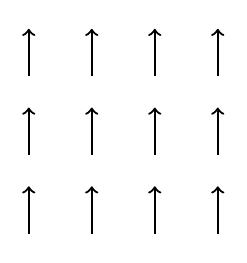
\begin{tikzpicture}
            \foreach \x in {0,...,3}{
                \foreach \y in {0,1,2}{
                    \draw[->,thick] (0.8*\x,\y-0.3)--(0.8*\x,\y+0.3);
                }
            }
        \end{tikzpicture}
    \end{figure}
    \\Each of these ground states has energy \(E=E_0=-2NJ\).

    The first excited states arise by flipping a single spin. Each spin has \(q=4\) nearest neighbours --- denoted by red lines in the example below --- each of which leads to an energy cost of \(J-(-J)=2J\). The energy of the first excited states is therefore \(E_1=E_0+8J\).
    \begin{figure}[ht!]
        \centering
        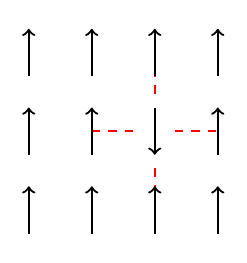
\begin{tikzpicture}
            \draw[dashed,thick,red] (1.6,0)--(1.6,2);
            \draw[dashed,thick,red] (0.8,1)--(2.4,1);
            \foreach \x in {0,...,3}{
                \foreach \y in {0,1,2}{
                    \draw[->,thick] (0.8*\x,\y-0.3)--(0.8*\x,\y+0.3);
                }
            }
            \fill[white] (1.4,0.6) rectangle (1.8,1.4);
            \draw[<-,thick] (1.6,0.7)--(1.6,1.3);
        \end{tikzpicture}
    \end{figure}
    \\There are, of course, \(N\) different spins that we can flip and, correspondingly, the first energy level has a degeneracy of \(N\).

    To proceed, we introduce a diagrammatic method to list the different states. We draw only the broken bonds which connect two spins with opposite orientation and, as in the diagram above, denote these by red lines. We further draw the flipped spins as red dots, the unflipped spins as blue dots. The energy of the state is determined simply by the number of red lines in the diagram. Pictorially, we write the first excited state as
    \begin{figure}[ht!]
        \centering
        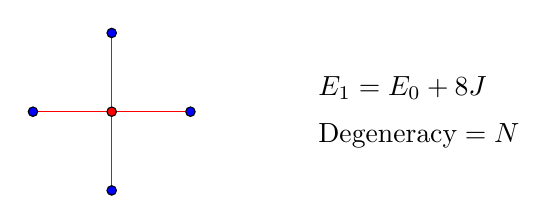
\begin{tikzpicture}
            \draw[red] (-1,0)--(1,0);
            \draw[red] (0,-1)--(0,1);
            \draw[fill=red] (0,0) circle (0.06);
            \draw[fill=blue] (1,0) circle (0.06);
            \draw[fill=blue] (-1,0) circle (0.06);
            \draw[fill=blue] (0,1) circle (0.06);
            \draw[fill=blue] (0,-1) circle (0.06);
            \node at (2.5,0.3)[right]{\(E_1=E_0+8J\)};
            \node at (2.5,-0.3)[right]{\(\text{Degeneracy}=N\)};
        \end{tikzpicture}
    \end{figure}

    The next lowest state has six broken bonds. It takes the form
    \begin{figure}[ht!]
        \centering
        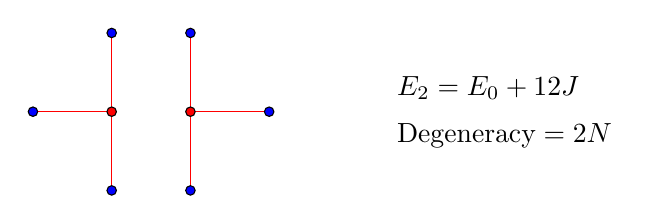
\begin{tikzpicture}
            \draw[red] (0,-1)--(0,1);
            \draw[red] (1,-1)--(1,1);
            \draw[red] (-1,0)--(0,0);
            \draw[red] (1,0)--(2,0);
            \foreach \x in {0,1}{
                \draw[fill=red] (\x,0) circle (0.06);
                \draw[fill=blue] (\x,-1) circle (0.06);
                \draw[fill=blue] (\x,1) circle (0.06);
                \draw[fill=blue] (3*\x-1,0) circle (0.06);
            }
            \node at (3.5,0.3)[right]{\(E_2=E_0+12J\)};
            \node at (3.5,-0.3)[right]{\(\text{Degeneracy}=2N\)};
        \end{tikzpicture}
    \end{figure}
    where the extra factor of \(2\) in the degeneracy comes from the two possible orientations (vertical and horizontal) of the graph.

    Things are more interesting for the states which sit at the third excited level. These have 8 broken bonds. The simplest configuration consists of two, disconnected, flipped spins
    \begin{equation}\label{disconnected_ising_graph}
        \tikz{
            \foreach \x in {0,1}{
                \draw[red] (3*\x-1,0)--(3*\x+1,0);
                \draw[red] (3*\x,-1)--(3*\x,1);
                \draw[fill=red] (3*\x,0) circle (0.06);
                \draw[fill=blue] (3*\x+1,0) circle (0.06);
                \draw[fill=blue] (3*\x-1,0) circle (0.06);
                \draw[fill=blue] (3*\x,1) circle (0.06);
                \draw[fill=blue] (3*\x,-1) circle (0.06);
            }
            \node at (5.5,0.3)[right]{\normalsize \(E_3=E_0+16J\)};
            \node at (5.5,-0.3)[right]{\normalsize \(\text{Degeneracy}=\frac{1}{2}N(N-5)\)};
        }
    \end{equation}
    The factor of \(N\) in the degeneracy comes from placing the first graph; the factor of \(N-5\) arises because the flipped spin in the second graph can sit anywhere apart from on the five vertices used in the first graph. Finally, the factor of \(1/2\) arises from the interchange of the two vertices.
    
    There are also three further graphs with the same energy \(E_3\). These are
    \begin{figure}[ht!]
        \centering
        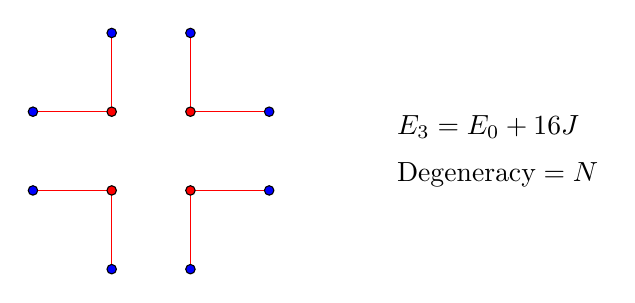
\begin{tikzpicture}
            \foreach \i in {1,-1}{
                \foreach \j in {1,-1}{
                    \draw[red] (0.5*\i,0.5*\j)--(1.5*\i,0.5*\j);
                    \draw[red] (0.5*\i,0.5*\j)--(0.5*\i,1.5*\j);
                    \draw[fill=red] (0.5*\i,0.5*\j) circle (0.06);
                    \draw[fill=blue] (1.5*\i,0.5*\j) circle (0.06);
                    \draw[fill=blue] (0.5*\i,1.5*\j) circle (0.06);
                }
            }
            \node at (3,0.3)[right]{\(E_3=E_0+16J\)};
            \node at (3,-0.3)[right]{\(\text{Degeneracy}=N\)};
        \end{tikzpicture}
    \end{figure}
    and
    \begin{figure}[ht!]
        \centering
        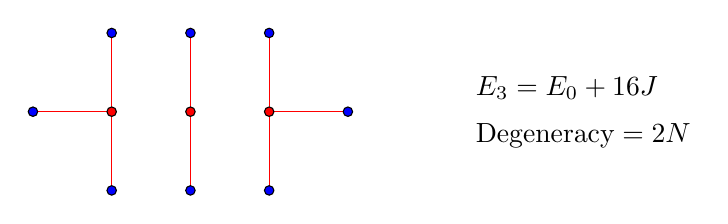
\begin{tikzpicture}
            \draw[red] (-1,0)--(0,0);
            \draw[red] (2,0)--(3,0);
            \foreach \x in {0,1,2}{
                \draw[red] (\x,-1)--(\x,1);
                \draw[fill=red] (\x,0) circle (0.06);
                \draw[fill=blue] (\x,-1) circle (0.06);
                \draw[fill=blue] (\x,1) circle (0.06);
            }
            \draw[fill=blue] (-1,0) circle (0.06);
            \draw[fill=blue] (3,0) circle (0.06);
            \node at (4.5,0.3)[right]{\(E_3=E_0+16J\)};
            \node at (4.5,-0.3)[right]{\(\text{Degeneracy}=2N\)};
        \end{tikzpicture}
    \end{figure}
    where the degeneracy comes from the two orientations, and finally
    \begin{figure}[ht!]
        \centering
        \begin{tikzpicture}
            \draw[red] (0,-1)--(0,1)--(2,1);
            \draw[red] (-1,0)--(0,0);
            \draw[red] (1,-1)--(1,0)--(2,0);
            \draw[red] (1,1)--(1,2);
            \draw[fill=red] (0,0) circle (0.06);
            \draw[fill=red] (1,0) circle (0.06);
            \draw[fill=red] (1,1) circle (0.06);
            \draw[fill=blue] (0,-1) circle (0.06);
            \draw[fill=blue] (1,-1) circle (0.06);
            \draw[fill=blue] (-1,0) circle (0.06);
            \draw[fill=blue] (2,0) circle (0.06);
            \draw[fill=blue] (2,1) circle (0.06);
            \draw[fill=blue] (1,2) circle (0.06);
            \draw[fill=blue] (0,1) circle (0.06);
            \node at (3.5,0.3)[right]{\(E_3=E_0+16J\)};
            \node at (3.5,-0.3)[right]{\(\text{Degeneracy}=4N\)};
        \end{tikzpicture}
    \end{figure}
    where the degeneracy comes from the four orientations.

    We can of course calculate more excited states but we will stop here. Adding all the graphs above gives us an expansion of the partition function in power of \(\ee^{-\beta J}\ll 1\). This is
    \begin{equation}\label{Ising_low_T_expansion}
        Q=2\ee^{2N\beta J}\left(1+N \ee^{-8\beta J}+2N\ee^{-12\beta J}+\frac{1}{2}(N^2+9N)\ee^{-16\beta J}+\dots\right)\,,
    \end{equation}
    where the overall factor of 2 originates from the two ground states of the system. We'll make use of the specific coefficients in this expansion in \cref{Chap:Kramers_Wannier}. Before we focus on the physics hiding in the low temperature expansion, it's worth making a quick comment that something quite nice happens if we take the log of the partition function and expand \(\ln(1+x)=x-\frac{1}{2}x^2+\dots\), we get
    \begin{equation}
        \ln Q = \ln 2+2N\beta J+N\ee^{-8\beta J}+2N\ee^{-12\beta J}+\frac{9}{2}N\ee^{-16\beta J}+\dots
    \end{equation}
    The thing to notice is that the \(N^2\) term in the partition function has precisely cancelled out and \(\ln Q\) is proportional to \(N\), which is to be expected since the free energy of the system is extensive. Looking back, we see that the \(N^2\) term was associated to the disconnected diagrams in (\ref{disconnected_ising_graph}). There is actually a general lesson hiding here: the partition function can be written as the exponential of the sum of connected diagrams. We saw exactly the same issue arise in the cluster expansion in (\ref{cluster_expansion_exp_sum}).

    \subsubsection*{Peierls Droplets}
    Continuing the low temperature expansion provides a heuristic, but physically intuitive, explanation for why phase transitions happen in \(d\ge 2\) dimensions but not in \(d=1\). As we flip more and more spins, the low energy states become \textit{droplets}, consisting of a region of space in which all the spins are flipped, surrounded by a larger sea in which the spins have their original alignment. The energy cost of such a droplet is roughly
    \begin{equation}
        E\sim 2JL\,,
    \end{equation}
    where \(L\) is the perimeter of the droplet. Notice that the energy does not scale as the area of the droplet since all spins inside are aligned with their neighbours. It is only those on the edge which are misaligned and this is the reason for the perimeter scaling. To understand how these droplets contribute to the partition function, we also need to know their degeneracy. We will now argue that the degeneracy of droplets scales as
    \begin{equation}
        \text{Degeneracy}\sim \ee^{\alpha L}
    \end{equation}
    for some value of \(\alpha\). To see this, consider firstly the problem of a random walk on a 2D square lattice. At each step, we can move in one of four directions. So the number of paths of length \(L\) is
    \begin{equation}
        \#\text{paths}\sim 4^L=\ee^{L\ln 4}\,.
    \end{equation}
    Of course, the perimeter of a droplet is more constrained than a random walk. Firstly, the perimeter can't go back on itself, so it really only has three directions that it can move in at each step. Secondly, the perimeter must return to its starting point after \(L\) steps. And, finally, the perimeter cannot self-intersect. One can show that the number of paths that obey these conditions is
    \begin{equation}
        \#\text{paths}\sim \ee^{\alpha L}\,,
    \end{equation}
    where \(\ln 2<\alpha<\ln 3\). Since the degeneracy scales as \(\ee^{\alpha L}\), the entropy of the droplets is proportional to \(L\).

    The fact that both energy and entropy scale with \(L\) means that there is an interesting competition between them. At temperatures where the droplets are important, the partition function is schematically of the form
    \begin{equation}
        Q\sim \sum_L \ee^{\alpha L}\ee^{-2\beta JL}\,.
    \end{equation}
    For large \(\beta\) (i.e. low temperature) the partition function converges. However, as the temperature increases, one reaches the critical temperature
    \begin{equation}\label{peierls_droplets_tc}
        k_B T_c\approx\frac{2J}{\alpha}
    \end{equation}
    where the partition function no longer converges. At this point, the entropy wins over the energy cost and it is favourable to populate the system with droplets of arbitrary sizes. This is how one sees the phase transition in the partition function. For temperature above \(T_c\), the low-temperature expansion breaks down and the ordered magnetic phase is destroyed.

    We can also use the droplet argument to see why phase transitions don't occur in \(d=1\) dimension. On a line, the boundary of any droplet always consists of just two points. This means that the energy cost to forming a droplet is always \(E=2J\), regardless of the size of the droplet. But, since the droplet can exist anywhere along the line, its degeneracy is \(N\). The net result is that the free energy associated to creating a droplet scales as
    \begin{equation}
        A=2J-k_B T\ln N
    \end{equation}
    and, as \(N\to\infty\), the free energy is negative for any \(T>0\). This means that the system will prefer to create droplets of arbitrary length, randomizing the spins. This is the intuitive reason why there is no magnetic ordered phase in the \(d=1\) Ising model.

    \subsubsection{High Temperature Limit}
    We now turn to the 2D Ising model in the opposite limit of high temperature. Here we expect the partition function to be dominated by the completely random, disordered configurations of maximum entropy. Our goal is to find a way to expand the partition function in \(\beta J\ll 1\).

    We again work with zero magnetic field, \(B=0\) and write the partition function as
    \begin{equation}
        Q=\sum_{(s_i)}\exp\left(\beta J\sum_{\langle ij\rangle}s_i s_j\right)=\sum_{(s_i)}\prod_{\langle ij\rangle}\ee^{\beta Js_i s_j}\,.
    \end{equation}
    There is a useful way to rewrite \(\ee^{\beta Js_is_j}\) which relies on the fact that the product \(s_i s_j\) only takes \(\pm 1\). It doesn't take long to check the following identity:
    \begin{align}
        \ee^{\beta Js_is_j}&=\cosh\beta J+s_i s_j\sinh\beta J\notag \\
        &=\cosh\beta J(1+s_is_j\tanh\beta J)\,.
    \end{align}
    Using this, the partition function becomes
    \begin{align}
        Q&=\sum_{(s_i)}\prod_{\langle ij\rangle}\cosh\beta J(1+s_is_j\tanh\beta J)\notag\\
        &=(\cosh\beta J)^{qN/2}\sum_{(s_i)}\prod_{\langle ij\rangle}(1+s_is_j\tanh\beta J)\,,\label{Ising_high_T_partition_function}
    \end{align}
    where the number of nearest neighbours is \(q=4\) for the 2D square lattice.

    With the partition function in this form, there is a natural expansion which suggests itself. At high temperatures \(\beta J\ll 1\) which, of course, means that \(\tanh\beta J\ll 1\). But the partition function is now naturally a product of powers of \(\tanh\beta J\). This is again somewhat analogous to the cluster expansion for the interacting gas. As in the cluster expansion, we will represent the expansion graphically.

    We need no graphics for the leading order term. It has no factors of \(\tanh \beta J\) and is simply
    \begin{equation}
        Q\approx(\cosh\beta J)^{2N}\sum_{(s_i)}1=2^N(\cosh\beta J)^{2N}\,.
    \end{equation}

    Let's now turn to the leading correction. Expanding the partition function (\ref{Ising_high_T_partition_function}), each power of \(\tanh \beta J\) is associated to a nearest neighbour pair \(\langle i,j\rangle\). We'll represent this by drawing a line on the lattice:
    \begin{equation}
        \tikz[baseline=-0.25 em]{
            \draw (0,0)circle (0.06);
            \draw (1,0)circle (0.06);
            \node at (0,0)[left] {\small \(i\)};
            \node at (1,0)[right] {\small \(j\)};
            \draw (0.06,0)--(0.94,0);
        }=s_is_j\tanh\beta J\,.
    \end{equation}
    But a sum over graphs of these kinds vanishes: each factor of \(\tanh\beta J\) in (\ref{Ising_high_T_partition_function}) also comes with a sum over all spins \(s_i\) and \(s_j\). And these are \(+1\) and \(-1\) which means that they simply sum to zero
    \begin{equation}
        \sum_{s_i,s_j}s_i s_j=+1-1-1+1=0\,.
    \end{equation}
    How can we avoid this? The only way is to make sure that we're summing over an even number of spins on each site, since then we get factors of \(s_i^2=1\) and no cancellations. Graphically, this means that every site must have an even number of lines attached to it. The first correction is then of the form
    \begin{equation}
        \tikz[baseline=0 em]{
            \draw (-0.5,0.5) circle (0.06) node[left]{\small 1};
            \draw (0.5,0.5) circle (0.06) node[right]{\small 2};
            \draw (0.5,-0.5) circle (0.06) node[right]{\small 3};
            \draw (-0.5,-0.5) circle (0.06) node[left]{\small 4};
            \draw (-0.44,0.5)--(0.44,0.5);
            \draw (0.5,0.44)--(0.5,-0.44);
            \draw (-0.44,-0.5)--(0.44,-0.5);
            \draw (-0.5,0.44)--(-0.5,-0.44);
        }=(\tanh\beta J)^4\sum_{(s_i)}s_1s_2\, s_2s_3\, s_3s_4\, s_4s_1=2^4(\tanh\beta J)^4\,.
    \end{equation}
    There are \(N\) such terms since the upper left corner of the square can be on any one of the \(N\) lattice sites (assuming periodic boundary conditions for the lattice). So including the leading term and first correction, we have
    \begin{equation}
        Q=2^N(\cosh\beta J)^{2N}(1+N(\tanh\beta J)^4+\dots)\,.
    \end{equation}

    We can go further. The next terms arise from graphs of length 6 and the only possibilities are rectangles, oriented as either landscape or portrait. Each of them can sit on one of \(N\) sites, giving a contribution
    \begin{equation}
        \tikz[baseline=1 em]{
            \draw (0,0) rectangle (2,1);
            \foreach \x in {0,1,2}{
                \foreach \y in {0,1}{
                    \draw[fill=white] (\x,\y) circle (0.06);
                }
            }
        } \ + \ \tikz[baseline=2.1 em]{
            \draw (0,0) rectangle (1,2);
            \foreach \x in {0,1}{
                \foreach \y in {0,1,2}{
                    \draw[fill=white] (\x,\y) circle (0.06);
                }
            }
        }\ =2N(\tanh\beta J)^6\,.
    \end{equation}

    Things get more interesting when we look at graphs of length 8. We have four different types of graphs. Firstly, there are the trivial, disconnected pair of squares
    \begin{equation}
        \tikz[baseline=1 em]{
            \draw (0,0) rectangle (1,1);
            \foreach \x in {0,1}{
                \foreach \y in {0,1}{
                    \draw[fill=white] (\x,\y) circle (0.06);
                }
            }
            \draw (2,0) rectangle (3,1);
            \foreach \x in {2,3}{
                \foreach \y in {0,1}{
                    \draw[fill=white] (\x,\y) circle (0.06);
                }
            }
        }\ =\frac{1}{2}N(N-5)(\tanh\beta J)^8\,.
    \end{equation}
    Here the first factor of \(N\) is the possible positions of the first square; the factor of \(N-5\) arises because there are 5 locations the second square can't be: overlapping or neighbouring with the first square. Finally, the factor of \(1/2\) comes because the two squares are identical. The other graphs of length 8 are a large square, a rectangle and a corner.
    \begin{equation}
        \tikz[baseline=2.1 em]{
            \draw (0,0) rectangle (2,2);
            \foreach \x in {0,1,2}{
                \foreach \y in {0,1,2}{
                    \draw[fill=white] (\x,\y) circle (0.06);
                }
            }
            \fill[white] (0.9,0.9) rectangle (1.1,1.1);
        } \ =N(\tanh\beta J)^8\,,
    \end{equation}
    \begin{equation}
        \tikz[baseline=1 em]{
            \draw (0,0) rectangle (3,1);
            \foreach \x in {0,1,2,3}{
                \foreach \y in {0,1}{
                    \draw[fill=white] (\x,\y) circle (0.06);
                }
            }
        } \ =2N(\tanh\beta J)^8
    \end{equation}
    and
    \begin{equation}
        \tikz[baseline=2.1 em]{
            \draw (0,0)--(2,0)--(2,2)--(1,2)--(1,1)--(0,1)--(0,0);
            \foreach \x in {0,1,2}{
                \foreach \y in {0,1,2}{
                    \draw[fill=white] (\x,\y) circle (0.06);
                }
            }
            \fill[white] (-0.1,1.9) rectangle (0.1,2.1);
        }\ =4N(\tanh\beta J)^8\,.
    \end{equation}
    Adding all contributions together gives us the first few terms in high temperature expansion of the partition function
    \begin{align}
        Q=2^N(\cosh\beta J)^{2N}\Big(1&+N(\tanh\beta J)^4+2N(\tanh\beta J)^6\notag\\
        &\qquad+\frac{1}{2}(N^2+9N)(\tanh\beta J)^8+\dots\Big)\,.\label{Ising_high_T_expansion}
    \end{align}
    You might have already noticed, everything above are weirdly familiar to everything in the low temperature expansion.

    \subsubsection{Kramers--Wannier Duality}\label{Chap:Kramers_Wannier}
    We have computed the partition function perturbatively in two extreme regimes of low temperature and high temperature. The physics in the two cases is, of course, very different. At low temperatures, the partition function is dominated by the lowest energy states; at high temperatures it is dominated by maximally disordered states. Yet comparing the partition functions at low temperature (\ref{Ising_low_T_expansion}) and high temperature (\ref{Ising_high_T_expansion}) reveals an extraordinary symmetry between them! The two series agree if we exchange
    \begin{equation}\label{Kramers_Wannier_Duality}
        \ee^{-2\beta J}\longleftrightarrow \tanh\beta J\,.
    \end{equation}
    Of course, we've only checked the agreement to the first few orders in perturbation. Below we shall prove that this miracle continues to all orders in perturbation theory. The symmetry of the partition function under the interchange (\ref{Kramers_Wannier_Duality}) is known as \textit{Kramers--Wannier duality}. Before we prove this duality, we will first just assume that it is true and extract some consequences.

    We can express the statement of the duality more clearly. The Ising model at temperature \(\beta\) is related to the same model at temperature \(\tilde{\beta}\), defined as
    \begin{equation}
        \ee^{-2\tilde{\beta}J}=\tanh\beta J\,.
    \end{equation}
    This way of writing things hides the symmetry of the transformation. A little algebra shows that this is equivalent to
    \begin{equation}
        \sinh 2\tilde{\beta}J=\frac{1}{\sinh 2\beta J}\,.
    \end{equation}
    This is a hot-cold duality --- when \(\beta\) is large, \(\tilde{\beta}\) is small. Kramers--Wannier duality is the statement that, when \(B=0\), the partition functions of the Ising model at two temperatures are related by
    \begin{align}
        Q(\beta)&=\frac{2^N(\cosh\beta J)^{2N}}{2\ee^{2N\tilde{\beta} J}}Q(\tilde{\beta})\notag \\
        &=2^{N-1}(\cosh\beta J\sinh\beta J)^N Q(\tilde{\beta})\,.
    \end{align}
    This means that if you know the thermodynamics of the Ising model at one temperature, then you also know the thermodynamics at the other temperature. Notice however, that it does not say that all the physics of the two models is equivalent. In particular, when one system is in the ordered phase, the other typically lies in the disordered phase.

    One immediate consequence of the duality is that we can use it to compute the exact critical temperature \(T_c\). This is the temperature at which the partition function is singular in the \(N\to\infty\) limit. If we further assume that there is just a single phase transition as we vary the temperature, then it must happen at the special self-dual point \(\beta=\tilde{\beta}\). This is
    \begin{equation}
        k_B T=\frac{2J}{\ln(\sqrt{2}+1)}\approx 2.269J\,.
    \end{equation}
    The exact solution of Onsager confirms that this is indeed the transition temperature. It's also worth noting that it's fully consistent with the more heuristic Peierls droplet argument (\ref{peierls_droplets_tc}) since \(\ln 2 < \ln(1+\sqrt{2}) < \ln 3\).

    \subsubsection*{Proving the Kramers--Wannier Duality}
    The key idea that we need can actually be found in the various graphs that we have drawn. You may have realised that the graphs we have drawn in the two expansions are actually the same, albeit drawn differently. For example, consider the two ``corner'' diagrams
    \begin{figure}[ht!]
        \centering
        \begin{tikzpicture}
            \draw[red] (0,-1)--(0,1)--(2,1);
            \draw[red] (-1,0)--(0,0);
            \draw[red] (1,-1)--(1,0)--(2,0);
            \draw[red] (1,1)--(1,2);
            \draw[fill=red] (0,0) circle (0.06);
            \draw[fill=red] (1,0) circle (0.06);
            \draw[fill=red] (1,1) circle (0.06);
            \draw[fill=blue] (0,-1) circle (0.06);
            \draw[fill=blue] (1,-1) circle (0.06);
            \draw[fill=blue] (-1,0) circle (0.06);
            \draw[fill=blue] (2,0) circle (0.06);
            \draw[fill=blue] (2,1) circle (0.06);
            \draw[fill=blue] (1,2) circle (0.06);
            \draw[fill=blue] (0,1) circle (0.06);

            \node at (3.5,0.5) {vs};

            \draw (5,-0.5)--(7,-0.5)--(7,1.5)--(6,1.5)--(6,0.5)--(5,0.5)--(5,-0.5);
            \foreach \x in {5,6,7}{
                \foreach \y in {-0.5,0.5,1.5}{
                    \draw[fill=white] (\x,\y) circle (0.06);
                }
            }
            \fill[white] (4.9,1.4) rectangle (5.1,1.6);
        \end{tikzpicture}
    \end{figure}
    \\The two graphs are \textit{dual}. The red lines in the first graph intersect the black lines in the second as can be seen by placing them on top of each other:
    \begin{figure}[ht!]
        \centering
        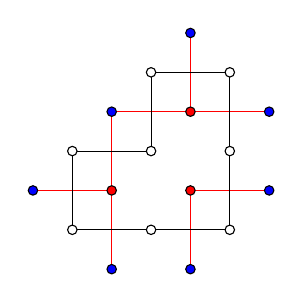
\begin{tikzpicture}
            \draw[red] (0,-1)--(0,1)--(2,1);
            \draw[red] (-1,0)--(0,0);
            \draw[red] (1,-1)--(1,0)--(2,0);
            \draw[red] (1,1)--(1,2);
            \draw[fill=red] (0,0) circle (0.06);
            \draw[fill=red] (1,0) circle (0.06);
            \draw[fill=red] (1,1) circle (0.06);
            \draw[fill=blue] (0,-1) circle (0.06);
            \draw[fill=blue] (1,-1) circle (0.06);
            \draw[fill=blue] (-1,0) circle (0.06);
            \draw[fill=blue] (2,0) circle (0.06);
            \draw[fill=blue] (2,1) circle (0.06);
            \draw[fill=blue] (1,2) circle (0.06);
            \draw[fill=blue] (0,1) circle (0.06);
            \draw (-0.5,-0.5)--(1.5,-0.5)--(1.5,1.5)--(0.5,1.5)--(0.5,0.5)--(-0.5,0.5)--(-0.5,-0.5);
            \foreach \x in {-0.5,0.5,1.5}{
                \foreach \y in {-0.5,0.5,1.5}{
                    \draw[fill=white] (\x,\y) circle (0.06);
                }
            }
            \fill[white] (-0.6,1.4) rectangle (-0.4,1.6);
        \end{tikzpicture}
    \end{figure}
    \\The same pattern occurs more generally: the graphs appearing in the low temperature expansion are in one-to-one correspondence with the dual graphs of the high temperature expansion. Here we will show how this occurs and how one can map the partition functions onto each other.
    
    Let's start by writing the partition function in the form (\ref{Ising_high_T_partition_function}) that we met in the high temperature expansion and presenting it in a slightly different way,
    \begin{align}
        Q(\beta)&=\sum_{(s_i)}\prod_{\langle ij\rangle}(\cosh\beta J+s_i s_j\sinh\beta J)\notag\\
        &=\sum_{(s_i)}\prod_{\langle ij\rangle}\sum_{k_{ij}=0,1}C_{k_{ij}}(\beta J)(s_i s_j)^{k_{ij}}\,,
    \end{align}
    where we have introduced the rather strange variable \(k_{ij}\) associated to each nearest neighbour pair that takes values 0 and 1, together with the functions
    \begin{equation}
        C_0(\beta J)=\cosh\beta J\qquad\text{and}\qquad C_1(\beta J)=\sinh\beta J\,.
    \end{equation}
    The variables in the original Ising model were spins on the lattice sites. The observation that the graphs which appear in the two expansions are dual suggests that it might be profitable to focus attention on the links between lattice sites. Clearly, we have one link for every nearest neighbour pair. If we label these links by \(\ell\), we can trivially rewrite the partition function as
    \begin{equation}
        Q=\sum_{k_\ell=0,1}\prod_{\ell}\sum_{(s_i)}C_{k_\ell}(\beta J)(s_is_j)^{k_\ell}\,.
    \end{equation}
    Notice that the strange label \(k_{ij}\) has now become a variable that lives on the links \(\ell\) rather than the original lattice sites \(i\).

    At this stage, we do the sum over the spins \(s_i\). We've already seen that if a given spin, say \(s_i\), appears in a term an odd number of times, then that term will vanish when we sum over the spin. Alternatively, if the spin \(s_i\) appears an even number of times, then the sum will give 2. We'll say that a given link \(\ell\) is turned on in configurations with \(k_\ell = 1\) and turned off when \(k_\ell = 0\). In this language, a term in the sum over spin \(s_i\) contributes only if an even number of links attached to site \(i\) are turned on. The partition function then becomes
    \begin{equation}\label{ising_constrained_partition_function}
        Q=2^N\left.\sum_{k_\ell}\prod_{\ell}C_{k_\ell}(\beta J)\right|_{\text{constrained}}\,.
    \end{equation}
    Now we have something interesting. Rather than summing over spins on lattice sites, we're now summing over the new variables \(k_\ell\) living on links. This looks like the partition function of a totally different physical system, where the degrees of freedom live on the links of the original lattice. But there's a catch --- that ``constrained'' label on the sum. This is there to remind us that we don't sum over all \(k_\ell\) configurations; only those for which an even number of links are turned on for every lattice site. And that's annoying. It's telling us that the \(k_\ell\) aren't really independent variables. There are some constraints that must be imposed.

    Fortunately, for the 2D square lattice, there is a simple way to solve the constraint. We introduce yet more variables, \(\tilde{s}_i\) which, like the original spin variables, take values \(\pm 1\). However, the \(\tilde{s}_i\) do not live on the original lattice sites. Instead, they live on the vertices of the dual lattice. For the 2D square lattice, the dual vertices are drawn in the figure. The original lattice sites are in white; the dual lattice sites in black.
    \begin{figure}
        \centering
        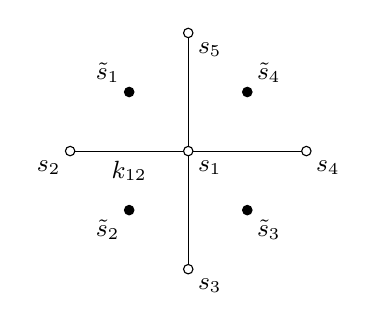
\begin{tikzpicture}
            \draw (-1.5,0)--(1.5,0);
            \draw (0,-1.5)--(0,1.5);
            \draw[fill=white] (0,0) node[below right]{\small\(s_1\)} circle (0.06);
            \draw[fill=white] (-1.5,0) node[below left]{\small\(s_2\)} circle (0.06);
            \draw[fill=white] (0,-1.5) node[below right]{\small\(s_3\)} circle (0.06);
            \draw[fill=white] (1.5,0) node[below right]{\small\(s_4\)} circle (0.06);
            \draw[fill=white] (0,1.5) node[below right]{\small\(s_5\)} circle (0.06);
            \draw[fill=black] (-0.75,0.75) node[above left]{\small\(\tilde{s}_1\)} circle (0.06);
            \draw[fill=black] (-0.75,-0.75) node[below left]{\small\(\tilde{s}_2\)} circle (0.06);
            \draw[fill=black] (0.75,0.75) node[above right]{\small\(\tilde{s}_4\)} circle (0.06);
            \draw[fill=black] (0.75,-0.75) node[below right]{\small\(\tilde{s}_3\)} circle (0.06);
            \node at (-0.75,0)[below]{\small\(k_{12}\)};
        \end{tikzpicture}
    \end{figure}

    The link variables \(k_\ell\) are related to the two nearest (dual) spin variables \(\tilde{s}_i\) as follows:
    \begin{align}
        k_{12}&=\frac{1}{2}(1-\tilde{s}_1\tilde{s}_2)\\
        k_{13}&=\frac{1}{2}(1-\tilde{s}_2\tilde{s}_3)\\
        k_{14}&=\frac{1}{2}(1-\tilde{s}_3\tilde{s}_4)\\
        k_{15}&=\frac{1}{2}(1-\tilde{s}_1\tilde{s}_4)
    \end{align}
    Notice that we've replaced four variables \(k_\ell\) taking values \(0,1\) with four variables \(\tilde{s}_i\) taking values \(\pm1\). Each set of variables gives \(2^4\) possibilities. However, the map is not one-to-one. It is not possible to construct for all values of \(k_\ell\) using the parameterization in terms of \(\tilde{s}_i\). To see this, we need only look at
    \begin{align}
        k_{12}+k_{13}+k_{14}+k_{15}&=2-\frac{1}{2}(\tilde{s}_1\tilde{s}_2+\tilde{s}_2\tilde{s}_3+\tilde{s}_3\tilde{s}_4+\tilde{s}_1\tilde{s}_4)\notag \\
        &=2-\frac{1}{2}(\tilde{s}_1+\tilde{s}_3)(\tilde{s}_2+\tilde{s}_4)\notag \\
        &=0,2\text{ or }4\,.
    \end{align}
    In other words, the number of links that are turned on must be even. But that's exactly what we want! Writing the \(k_\ell\) in terms of the auxiliary spins \(\tilde{s}_i\) automatically solves the constraint that is imposed on the sum in (\ref{ising_constrained_partition_function}). Moreover, it is simple to check that for every configuration \(\{k_\ell\}\) obeying the constraint, there are two configurations of \(\{\tilde{s}_i\}\). This means that we can replace the constrained sum over \(\{k_\ell\}\) with an unconstrained sum over \(\{\tilde{s}_i\}\). The only price we pay is an additional factor of \(1/2\).
    \begin{equation}
        Q(\beta)=\frac{1}{2}2^N\sum_{(\tilde{s}_i)}\prod_{\langle ij\rangle}C_{\frac{1}{2}(1-\tilde{s}_i\tilde{s}_j)}(\beta J)\,.
    \end{equation}
    Finally, we'd like to find a simple expression for \(C_0\) and \(C_1\) in terms of \(\tilde{s}_i\). That's easy enough. We can write
    \begin{align}
        C_k(\beta J)&=\cosh\beta J\exp(k\ln\tanh\beta J)\notag\\
        &=(\sinh\beta J\cosh\beta J)^{1/2}\exp\left(-\frac{1}{2}\tilde{s}_i\tilde{s}_j\ln\tanh\beta J\right)\,.
    \end{align}
    Substituting this into our newly re-written partition function gives
    \begin{align}
        Q(\beta)&=2^{N-1}\sum_{(\tilde{s}_i)}\prod_{\langle ij\rangle}(\sinh\beta J\cosh\beta J)^{1/2}\exp\left(-\frac{1}{2}\tilde{s}_i\tilde{s}_j\ln\tanh\beta J\right)\notag \\
        &=2^{N-1}(\sinh\beta J\cosh\beta J)^{N}\sum_{(\tilde{s}_i)}\exp\left(-\frac{1}{2}\ln(\tanh\beta J)\sum_{\langle ij\rangle}\tilde{s}_i\tilde{s}_j\right)\,.
    \end{align}
    This final form of the partition function in terms of the dual spins \(\tilde{s}_i\) has exactly the same functional form as the original partition function in terms of the spins \(s_i\)! More precisely, we can write
    \begin{equation}
        Q(\beta)=2^{N-1}(\sinh 2\beta J)^N Q(\tilde{\beta})\,,
    \end{equation}
    where
    \begin{equation}
        \ee^{-2\tilde{\beta}J}=\tanh\beta J
    \end{equation}
    as advertised. This is the Kramers--Wannier duality.

    This seems to be too out of a tangent from our main theme, but the concept of \textit{duality} is a major feature in theoretical research. The key idea is that when the temperature gets large there may be a different set of variables in which a theory can be written where it appears to live at low temperature. The same idea often holds in quantum theories, where duality maps strong coupling problems to weak coupling problems.

    The duality in the Ising model is special for two reasons: firstly, the new variables \(\tilde{s}_i\) are governed by the same Hamiltonian as the original variables \(s_i\). We say that the Ising model is \textit{self-dual}. In general, this need not be the case --- the high temperature limit of one system could look like the low-temperature limit of a very different system. Secondly, the duality in the Ising model can be proven explicitly. For most systems, we have no such luck. Nonetheless, the idea that there may be dual variables in other, more difficult theories, is compelling. Commonly studied examples include the exchange particles and vortices in two dimensions, and electrons and magnetic monopoles in three dimensions.

    \section{Lee--Yang Theorem}
    You may have noticed that the flavour of our discussion on phase transitions is a little different from the previous chapter. Our previous philosophy was to regard the partition function as the most important quantity that we can use to derive everything, but when doing phase transitions, we dumped the partition function as soon as we could, preferring instead to work with the macroscopic variable like the free energy. Why didn't we stick with the partition function and examine phase transitions directly?

    The reason is that the approach using the partition function is hard! In this short appendix section, which is somewhat tangential to our main discussion, we will describe how phase transitions manifest themselves in the partition function.

    For concreteness, let's go back to the classical non-ideal gas with pairwise-additive interactions, although the results we derive will be more general. We'll work in the grand canonical ensemble, with the partition function
    \begin{equation}
        \Xi=\sum_N z^N Q(N,V,T)=\sum_{N}\frac{z^N}{N!\Lambda^{3N}}\int\prod_{i}\dd[3]{\vb{r}_i}\ee^{-\beta\sum_{j<k}U(r_{jk})}\,.
    \end{equation}
    To regulate any potential difficulties with short distances, it is useful to assume that the particles have hard cores so that they cannot approach to a distance less than \(r_0\). We model this by requiring that the potential satisfies
    \begin{equation}
        U(r_{jk})=\infty\qquad\text{for }r_{jk}<r_0\,.
    \end{equation}
    But this has an obvious consequence: if the particles have finite size, then there is a maximum number of particles, \(N_V\), that we can fit into a finite volume \(V\). (Roughly this number is \(N_V\sim V/r_0^3\)). But that, in turn, means that the canonical partition function \(Q(N,V,T)=0\) for \(N>N_V\), and the grand partition function \(\Xi\) is therefore a finite polynomial in the fugacity \(z\), of order \(N_V\). But if the partition function is a finite polynomial, there can't be any discontinuous behaviour associated with a phase transition. In particular, we can calculate
    \begin{equation}
        PV=k_B T\ln\Xi\,,
    \end{equation}
    which gives us \(PV\) as a smooth function of \(z\). We can also calculate
    \begin{equation}\label{Xi_derivative}
        N=z\pdv{}{z}\ln\Xi\,,
    \end{equation}
    which gives us \(N\) as a function of \(z\). Eliminating \(z\) between these two functions tells us that pressure \(p\) is a smooth function of density \(N/V\). We're never going to get the behaviour that we derived from the Maxwell construction in which the plot of pressure against density shown in \cref{vdW_loops} exhibits a discontinuous derivative.

    The discussion above is just re-iterating a statement that we've alluded to before: there are no phase transitions in a finite system. To see the discontinuous behaviour, we need to take the limit \(V\to\infty\). A theorem due to Lee and Yang gives us a handle on the analytic properties of the partition function in this limit.

    The surprising insight of Lee and Yang is that if you're interested in phase transitions, you should look at the zeros of \(\Xi\) in the complex \(z\)-plane.\footnote{This probably isn't too surprising if you stare at the definition of canonical partition function long enough and suddenly realise that \(Q(N,V,T)\) is the (discrete) Laplace transform of \(\Omega(N,V,E)\).} Let's first look at these when \(V\) is finite. Importantly, at finite \(V\) there can be no zeros on the positive real axis, \(z>0\). This follows from the definition of \(\Xi\) where it is a sum of positive quantities. Moreover, from (\ref{Xi_derivative}), we can see that \(\Xi\) is a monotonically increasing function of \(z\) because we necessarily have \(N>0\). Nonetheless, \(\Xi\) is a polynomial in \(z\) of order \(N_V\) so it certainly has \(N_V\) zeros somewhere in the complex \(z\)-plane. Since \(\Xi^*(z)=\Xi(z^*)\), these zeros must either sit on the real negative axis or come in complex conjugate pairs.

    However, the statements above rely on the fact that \(\Xi\) is a finite polynomial. As we take the limit \(V\to\infty\), the maximum number of particles that we can fit in the system diverges, \(N_V\to\infty\), and \(\Xi\) is now defined as an infinite series. But infinite series can do things that finite ones can't. The Lee-Yang theorem says that as long as the zeros of \(\Xi\) continue to stay away from the positive real axis as \(V\to\infty\), then no phase transitions can happen. But if one or more zeros happen to touch the positive real axis, life gets more interesting.

    \begin{thm}[Lee--Yang Theorem]
        The quantity
        \begin{equation}
            \Theta\coloneqq\lim_{V\to\infty}\left[\frac{1}{V}\ln\Xi(z,V,T)\right]
        \end{equation}
        exists for all \(z>0\). The result is a continuous, non-decreasing function of \(z\) which is independent of the shape of the box (up to some sensible assumptions such as \(\text{Surface Area}/V\sim V^{-1/3}\) which ensures that the box isn't some stupid fractal shape).

        Moreover, let \(R\) be a fixed, volume independent, region in the complex \(z\) plane which contains part of the real, positive axis. If \(R\) contains no zero of \(\Xi(z,V,T)\) for all \(z\in R\), then \(\Theta\) is an analytic function of \(z\) for all \(z\in R\). In particular, all derivatives of \(\Theta\) are continuous.
    \end{thm}

    In other words, there can be no phase transitions in the region \(R\) even in the \(V\to\infty\) limit. The last result means that, as long as we are safely in a region \(R\), taking derivatives with respect to \(z\) commutes with taking the limit \(V\to\infty\). In other words, we are allowed to use (\ref{Xi_derivative}) to write the particle density \(\rho=N/V\) as
    \begin{equation}
        \lim_{V\to\infty}\rho=\lim_{V\to\infty}z\pdv{}{z}\left(\frac{P}{k_B T}\right)=z\pdv{\Theta}{z}\,.
    \end{equation}
    However, if we look at points \(z\) where zeros appear on the positive real axis, then \(\Theta\) will generally not be analytic. If \(\partial\Theta/\partial z\) is discontinuous, then the system is said to undergo a first order phase transition. More generally, if \(\partial^m\Theta/\partial z\) is discontinuous for \(m=n\), but continuous for all \(m<n\), then the system undergoes an \(n^{\text{th}}\) order phase transition.

    \section{Landau--Ginzburg Theory}\label{Chap:Landau_Ginzburg}
    Landau's theory of phase transition focuses only on the average quantity, the order parameter. It ignores the fluctuations of the system, assuming that they are negligible. Here we sketch a generalisation which attempts to account for these fluctuations. It is known as Landau--Ginzburg theory.

    The idea is to stick with the concept of order parameter \(m\), but now we allow the order parameter to vary in space so it becomes a function \(m(\vb{r})\). Let us restrict ourselves to the situation where there is a symmetry \(m\to -m\) so we only need to consider even powers in the expansion of the free energy. We add to these a gradient term whose role is to capture the fact that there is some stiffness in the system --- it costs energy to vary the order parameter from one point to another. (For the example of the Ising model, this is simply the statement that nearby spins want to be aligned). The (truncated) free energy is then given by
    \begin{equation}\label{Landau_Ginzburg_free_energy}
        A[m(\vb{r})]=\int\dd[d]{\vb{r}}[a(T)m^2+b(T)m^4+c(T)(\grad m)^2]\,.
    \end{equation}
    Notice that we start with terms quadratic in the gradient: a term linear in the gradient would violate the rotational symmetry of the system.

    We again require that the free energy is minimised. But now \(A\) is a functional --- it is a function of the function \(m(\vb{r})\). If you have learned variational principles, the stationary points will be given by the Euler--Lagrange equations. If you have not, long story short, we consider varying the function \(m(\vb{r})\) by \(\delta m(\vb{r})\). The variation of the free energy will then be
    \begin{align}
        \delta A&=\int\dd[d]{\vb{r}}[2am\delta m+4bm^3\delta m+2c\grad m\vdot\grad\delta m]\notag \\
        &=\int\dd[d]{\vb{r}}[2am+4bm^3-2c\laplacian m]\delta m\,,
    \end{align}
    where we used integration by parts. The minimum energy occurs when \(\delta A=0\) for any \(\delta m\) to the first order, and so
    \begin{equation}\label{Landau_Ginzburg}
        c\laplacian m=am+2bm^3\,.
    \end{equation}
    The simplest solution to this equation have \(m\) constant, reducing us back to Landau theory. However, allowing for the possibility of spatial variation in \(m\) opens up the possibility for us to search for some more interesting solutions.

    \subsection{Domain Walls}
    Suppose we have \(T<T_c\), the critical temperature, so there exists two degenerate ground states, \(m=\pm m_0\). We could cook up a situation in which one half of space, say \(x<0\), lives in the ground state \(m=-m_0\) while the other half of space, \(x>0\) lives in \(m=+m_0\). This is exactly analogous to the liquid--gas phase separation where we have a half liquid and a half gas. The two regions in which spins point up or down are called \textit{domains}. The place where these regions meet is called the \textit{domain wall}.

    We would like to understand the structure of the domain wall. How does the system interpolate between these two states? The transition can't happen instantaneously because that would result in the gradient term \((\grad m)^2\) giving an infinite contribution to the free energy. But neither can the transition linger too much because any point at which \(m(\vb{r})\) differs significantly from the value \(\pm m_0\) costs free energy from the \(m^2\) and \(m^4\) terms. There must be an equilibrium between these two effects.

    To describe the system with two domains, \(m(\vb{r})\) must vary, but it need only change in one direction: \(m=m(x)\). The equation (\ref{Landau_Ginzburg}) then reduces to an ordinary differential equation
    \begin{equation}
        \dv[2]{m}{x}=\frac{am}{c}+\frac{2bm^3}{c}\,.
    \end{equation}
    Remember we are below phase transition temperature, so \(a<0\). We then have
    \begin{equation}
        m=m_0\tanh\left(\sqrt{\frac{-a}{2c}}x\right)\,,
    \end{equation}
    where \(m_0=\sqrt{-a/2b}\) is the constant ground state solution for the spin. As \(x\to\pm\infty\), the \(\tanh\) function tends towards \(\pm 1\) which means that \(m\to\pm m_0\), so this solution indeed interpolates between the two domains as required. We learn that the width of the domain wall is given by \(\sqrt{-2c/a}\). Outside this region, the magnetisation relaxes exponentially quickly back to the ground state values.

    We can also compute the cost in free energy due to the presence of the domain wall. To do this, we substitute the solution back into the free energy expression. The cost is not proportional to the volume of the system, but instead proportional to the area of the domain wall. This means that if the system has a linear size \(L\) then the free energy of the ground state scales as \(L^d\) while the free energy required by the wall scales only as \(L^{d-1}\). It is simple to find the parametric dependence of this domain wall energy without doing any integrals; the energy per unit area scales as \(\sqrt{-ca^3/b}\). Notice that as we approach the critical point, and \(a\to 0\), the two vacua are closer, the width of the domain wall increases and its energy decreases.

    \subsection{Correlations}
    One of the most important applications of Landau--Ginzburg theory is to understand the correlations between fluctuations of the system at different points in space. Suppose that we know that the system has an unusually high fluctuation away from the average at some point in space, let's say the origin \(\vb{r}=\vb{0}\). What is the effect of this on nearby points?

    There is a simple way to answer this question that requires us only to solve the differential equation (\ref{Landau_Ginzburg}). However, there is also a more complicated way to derive the same result which has the advantage of stressing the underlying physics and the role played by fluctuations. We'll start by deriving the correlations in the simple manner. We'll then see how it can also be derived using the more technical machinery.

    We assume that the system sits in a given ground state, say \(m=+m_0\), and imagine a small perturbation around this. We write the magnetisation as
    \begin{equation}
        m(\vb{r})=m_0+\delta m(\vb{r})\,.
    \end{equation}
    If we substitute this into equation (\ref{Landau_Ginzburg}) and keep only terms linear in \(\delta m\), we find
    \begin{equation}
        c\laplacian\delta m+2a\delta m=0\,,
    \end{equation}
    where we have substituted \(m_0^2=-a/2b\). We now perturb the system. This can be modelled by putting a delta-function source at the origin, so that the above equation becomes
    \begin{equation}
        c\laplacian\delta m+2a\delta m=\frac{1}{2c}\delta(\vb{r})\,,
    \end{equation}
    where the strength of the delta function is chosen merely to make the equation somewhat nicer. It is straightforward to solve the asymptotic behaviour of this equation.\footnote{The same type of equation will arise in the Debye--H\"{u}ckel model of screening.} Neglecting constant factors, it is
    \begin{equation}
        \delta m(\vb{r})\sim\frac{\ee^{-r/\xi}}{r^{(d-1)/2}}\,.
    \end{equation}
    This tells us how the perturbation decays as we move away from the origin. This equation has several names, reflecting the fact that it arises in many contexts. In liquids, it is usually called the \textit{Ornstein--Zernicke correlation}. It also arises in particle physics as the \textit{Yukawa potential}. The length scale \(\xi\) is called the \textit{correlation length}
    \begin{equation}
        \xi=\sqrt{\frac{-c}{2a}}\,.
    \end{equation}
    It provides a measure of the distance it takes for correlations to decay. Notice that as we approach the critical point, \(a\to 0\) and the correlation length diverges. This provides yet another hint that we need more powerful tools to understand the physics at the critical point. We will now take the first step towards developing these tools.

    \subsection{Fluctuations}
    The main motivation to allow the order parameter to depend on space is to take into account the effect of fluctuations. To see how we can do this, we first need to think a little more about the meaning of the quantity \(A[m(\vb{r})]\) and what we can use it for.

    To understand this point, it is best if we go back to basics. We know that the true free energy of the system can be equated with the log of the partition function. The Landau--Ginzburg functional \(A[m(\vb{r})]\) is closely related to the true free energy, but it is not quite the same thing as we will see shortly. To avoid confusion, we will call the true free energy \(F\). Since \(F=-k_B T\ln Q\), we can write
    \begin{equation}
        \ee^{-\beta F}=Q=\sum_n \ee^{-\beta E_n}\,.
    \end{equation}
    We would like to understand the right way to view the functional \(A[m(\vb{r})]\) in this framework. Here we give a heuristic and fairly handwaving argument. A fuller treatment involves the idea of the renormalisation group, which you will learn if you decide to study statistical field theory.

    \begin{figure}
        \centering
        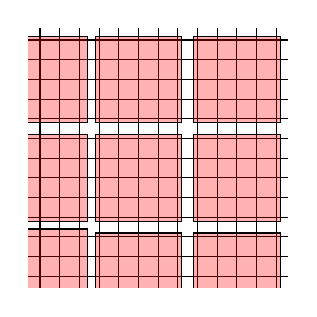
\begin{tikzpicture}
            \foreach \i in {0,...,12}{
                \draw (-0.15,0.25*\i)--(3.15,0.25*\i);
                \draw (0.25*\i,-0.15)--(0.25*\i,3.15);
            }
            \draw[fill=red,fill opacity=0.3] (-0.15,3.05)--(0.6,3.05)--(0.6,1.95)--(-0.15,1.95);
            \draw[fill=red,fill opacity=0.3] (-0.15,1.8)--(0.6,1.8)--(0.6,0.7)--(-0.15,0.7);
            \fill[red,opacity=0.3] (-0.15,-0.15) rectangle (0.6,0.6);
            \draw (-0.15,0.6)--(0.6,0.6)--(0.6,-0.15);
            \draw[fill=red,fill opacity=0.3] (0.7,1.95) rectangle (1.8,3.05);
            \draw[fill=red,fill opacity=0.3] (1.95,1.95) rectangle (3.05,3.05);
            \draw[fill=red,fill opacity=0.3] (0.7,0.7) rectangle (1.8,1.8);
            \draw[fill=red,fill opacity=0.3] (1.95,0.7) rectangle (3.05,1.8);
            \draw[fill=red,fill opacity=0.3] (0.7,-0.15)--(0.7,0.55)--(1.8,0.55)--(1.8,-0.15);
            \draw[fill=red,fill opacity=0.3] (1.95,-0.15)--(1.95,0.55)--(3.05,0.55)--(3.05,-0.15);
        \end{tikzpicture}
        \caption{Coarse graining in the Ising model lattice to define \(m(\vb{x})\).}
    \end{figure}

    The idea is that each microstate \(\ket{n}\) of the system can be associated to some specific function of the spatially varying order parameter \(m(\vb{r})\). To illustrate this, we'll talk in the language of the Ising model although the discussion generalises to any system. For the Ising model of \(N\) lattice points, we can divide the lattice into uniform blocks, each consisting of a number of lattice sites (say \(N'\) lattice points per box) but its scale should be smaller than any other length scales in our model (in particular, it should be smaller than the correlation length). This step is called \textit{coarse graining}. For each box, we can evaluate its average magnetisation \(m(\vb{r})=\frac{1}{N'}\sum_i s_i\), where \(\vb{r}\) is the centre of the box. Clearly this function is defined only at discrete points, if the number of boxes \(N/N'\) is big enough, we can effectively treat \(\vb{r}\) as being continuous. Moreover, at each \(\vb{r}\), \(m(\vb{r})\) is quantised in units of \(1/N'\), so we also need to take \(N'\) big enough so \(m(\vb{r})\) can effectively take any value between \(1\) and \(-1\).
    
    In this way, we get a map from the microstates to the magnetisation function, \(\ket{n}\to m(\vb{r})\). But due to the averaging process, this map is clearly not one-to-one. In this way, many microstates map onto the same average magnetisation. Summing over just these microstates provides a first principle construction of the \(A[m(\vb{r})]\):
    \begin{equation}\label{Landau_Ginzburg_free_energy_microstates}
        \ee^{-\beta A[m(\vb{r})]}=\sum_{n\mid m(\vb{r})}\ee^{-\beta E_n}\,.
    \end{equation}
    Of course, we didn't actually perform this procedure to get to (\ref{Landau_Ginzburg_free_energy}): we simply wrote it down the most general form in the vicinity of a critical point with a bunch of unknown coefficients \(a(T)\), \(b(T)\) and \(c(T)\). But if we were up for a challenge, the above procedure tells us how we could go about figuring out those functions from first principles. More importantly, it also tells us what we should do with the Landau--Ginzburg free energy. Because in (\ref{Landau_Ginzburg_free_energy_microstates}) we have only summed over those states that correspond to a particular value of \(m(\vb{r})\). To compute the full partition function, we need to sum over all states. But we can do that by summing over all possible values of \(m(\vb{r})\). In other words,
    \begin{equation}\label{partition_function_functional_integral}
        Q=\int\mathcal{D}m(\vb{r})\, \ee^{-\beta A[m(\vb{r})]}\,.
    \end{equation}
    This is a tricky beast: it is a functional integral. We are integrating over all possible functions \(m(\vb{r})\), which is the same thing as performing an infinite number of integrations. (Actually because the order parameter \(m(\vb{r})\) arose from an underlying lattice and are suitably smooth on short distance scales in our case, the problem is somewhat mitigated).

    The result (\ref{partition_function_functional_integral}) is physically very nice, albeit mathematically somewhat daunting. It means that we should view the Landau--Ginzburg free energy as an effective Hamiltonian for a continuous variable \(m(\vb{r})\), so that by integrating over all possible \(m(\vb{r})\), we get the partition function. It arises from performing the partition function sum over much of the microscopic information, but still leaves us with a final sum, or integral, over fluctuations in an averaged quantity, namely the order parameter.

    To complete the problem, we need to perform the functional integral (\ref{partition_function_functional_integral}). This is hard. Here ``hard'' means that the majority of the unsolved problems in theoretical physics can be boiled down to performing integrals of this type. Yet the fact it's hard shouldn't dissuade us, since there is a wealth of rich and beautiful physics hiding in the path integral, including the deep reason behind universality. You will explore this if you study statistical field theory.


    \section{An Introduction to Linear-Response Theory}\label{Chap:Intro_to_Linear_Response}
    We have derived a number of links between equilibrium properties and transport coefficients, specifically diffusion. We investigated how the approach of a system to equilibrium (diffusion of a particle) and the fluctuations at equilibrium (the root mean square distance travelled by a particle) turns out to be very closely related (by the Einstein relation). In fact, this relation is not limited to diffusion: there is a general set of relations known as \textit{Onsager reciprocal relations}, that express how ratios of flows and forces are related in near-equilibrium systems. We can extend out discussion slightly and formalise the link between equilibrium statistical mechanics and transport coefficients using what is known as the linear-response theory, and derive the relation between the mobility and the diffusion coefficient in another way still.

    We first note that the thermal average of an observable \(X\) is
    \begin{equation}
        \eval{X}=\frac{\int\dd{\Gamma}\ee^{-\beta H(\Gamma)X(\Gamma)}}{\int\dd{\Gamma}\ee^{-\beta H(\Gamma)}}\,,
    \end{equation}
    where we have denoted a point in the phase space by \(\Gamma=(\vb{p}_1,\dots,\vb{p}_N,\vb{r}_1,\dots,\vb{r}_N)\), and \(H=K+U\) is the total Hamiltonian. Now consider a small, linear perturbation \(\lambda B\), so that the perturbed Hamiltonian can be written as \(H=H^{(0)}+\lambda B\), where \(B\) is some field to be defined later and \(\lambda\) is its strength. We can then decompose the thermal average of \(X\) into its unperturbed part \(\eval{X}_0\) and a change due to the perturbation \(\Delta X\) such that
    \begin{equation}
        \eval{X}=\eval{X_0}+\eval{\Delta X}=\frac{\int\dd{\Gamma}\ee^{-\beta(H^{(0)}+\lambda B)}X}{\int\dd{\Gamma}\ee^{-\beta(H^{(0)}+\lambda B)}}\,.
    \end{equation}
    Now suppose \(\eval{X}\) is analytic in \(\lambda\), so that we can write
    \begin{equation}
        \eval{X}=\eval{X}_0+\left(\pdv{\eval{X}}{\lambda}\right)_{\lambda=0}\lambda+\frac{1}{2}\left(\pdv[2]{\eval{X}}{\lambda}\right)_{\lambda=0}\lambda^2+\dots
    \end{equation}
    We will focus on the linear response, i.e. the first order correction in the language of perturbation theory, and write
    \begin{equation}
        \eval{\Delta X}=\left(\pdv{\eval{X}}{\lambda}\right)_{\lambda=0}\lambda+O(\lambda^2)\,.
    \end{equation}
    We can find out an explicit expression for this simply by differentiating \(\eval{X}\) and get
    \begin{align}
        \pdv{\eval{X}}{\lambda}&=\frac{\int\dd{\Gamma}\pdv{}{\lambda}\ee^{-\beta(H^{(0)}+\lambda B)}X}{\int\dd{\Gamma}\ee^{-\beta(H^{(0)}+\lambda B)}}-\frac{\int\dd{\Gamma}\ee^{-\beta(H^{(0)}+\lambda B)}X}{[\int\dd{\Gamma}\ee^{-\beta(H^{(0)}+\lambda B)}]^2}\int\dd{\Gamma}\pdv{}{\lambda}\ee^{-\beta(H^{(0)}+\lambda B)}\notag \\
        &=-\beta\frac{\int\dd{\Gamma}\ee^{-\beta(H^{(0)}+\lambda B)}BX}{\int\dd{\Gamma}\ee^{-\beta(H^{(0)}+\lambda B)}}+\beta\frac{\int\dd{\Gamma}\ee^{-\beta(H^{(0)}+\lambda B)}X}{\int\dd{\Gamma}\ee^{-\beta(H^{(0)}+\lambda B)}}\frac{\int\dd{\Gamma}\ee^{-\beta(H^{(0)}+\lambda B)}B}{\int\dd{\Gamma}\ee^{-\beta(H^{(0)}+\lambda B)}}\notag\\
        &=-\beta[\eval{BX}-\eval{B}\eval{X}]\,.
    \end{align}
    We can evaluate this at \(\lambda=0\) to obtain the linear response to the perturbation
    \begin{equation}
        \eval{\Delta X}=-\beta\lambda[\eval{BX}_0-\eval{B}_0\eval{X}_0]+O((\beta\lambda B)^2)\,.
    \end{equation}

    As an example, let's consider the response of the polarisation \(\vb{P}\) of a system to a weak static electric field \(E_x\). The perturbative Hamiltonian is \(-E_xP_x\), so
    \begin{equation}
        \eval{\Delta P_x}=-\beta E_x[-\eval{P_xP_x}_0+\eval{P_x}_0\eval{P_x}_0]=\beta E_x[\eval{P_x^2}_0-\eval{P_x}_0^2]\,.
    \end{equation}
    The response to the external electric field therefore scales as \(\eval{P_x^2}_0-\eval{P_x}_0^2\). This is nothing other than the variance of the spontaneous polarisation without the electric field, which is a measure of the fluctuations of this property in the system at equilibrium. This is in fact quite a general result: the larger the spontaneous fluctuations a mechanical observable, the larger the response to an external field that is coupled to this observable.

    Let's now focus on a more general case of a system that we have equilibrated with an active perturbation with Hamiltonian \(H=H^{(0)}+\lambda B\), but we switch off this perturbation at time \(t=0\). For notational simplicity, we will assume that in the absence of the field, \(\eval{X}_0=0\). If this were not the case, we could simply define a new variable suitably shifted so that its average is zero, and we are not losing generality here. In classical mechanics, the motion is deterministic, and in the absence of an external force, the value of a mechanical observable at time \(t\) depends on the initial conditions, say at \(t=0\). Hence, we may evaluate the thermal average at time \(t\) using the integral of the phase space at \(t=0\),
    \begin{equation}
        \eval{\Delta X(t)}=\frac{\dd{\Gamma(0)}\ee^{-\beta(H^{(0)}+\lambda B)}X(t)}{\int\dd{\Gamma(0)}\ee^{-\beta(H^{(0)}+\lambda B)}}\,,
    \end{equation}
    where the Hamiltonian is evaluated at \(t=0\), where \(B=B(0)\) is at full strength. The remaining steps are exactly the same as above, and we get
    \begin{equation}
        \eval{\Delta X(t)}=-\beta\lambda[\eval{B(0)X(t)}_0-\eval{B(0)}_0\eval{X(t)}_0]\,.
    \end{equation}
    Since we have assumed that in the absence of the field, \(\eval{X}_0=0\), we are left with
    \begin{equation}\label{response_per_switched_on}
        \eval{\Delta X(t)}=-\beta\lambda\eval{B(0)X(t)}_0=-\beta\lambda C_{XB}(t)\,,
    \end{equation}
    where \(C_{XB}(t)\coloneqq\eval{B(0)X(t)}_0\) is the correlation function relating the mechanical property \(X\) at time \(t\) to the perturbative field \(B\) at times \(t=0\). For example, in the case of the weak electric field we considered above, when the field is on, there is a net polarisation \(P_x(0)\), but the field is switched off, then polarisation decays to zero as \(\eval{P_x(t)}=\beta E_x\eval{P_x(0)P_x(t)}\), where \(\eval{P_x(0)P_x(t)}\) is the dipole autocorrelation function.

    Finally, in order to make a link to the Einstein--Smoluchowski relation, we need to go one step further. Suppose that we write our perturbed Hamiltonian as \(H=H^{(0)}+\lambda(t)B\), where \(\lambda(t)\) is some function of time that governs the extent to which the perturbation is switched on. In general, we can write the response of the mechanical property \(X\) to the linear order in \(\lambda\) as
    \begin{equation}
        \eval{\Delta X(t)}=\int_{-\infty}^{\infty}\dd{t'}\chi_{XB}(t,t')\lambda(t')\,,
    \end{equation}
    where the response function \(\chi_{XB}(t,t')\) is to be determined. There are two properties we require of this function:
    \begin{itemize}
        \item The response must be \textit{causal}, i.e. the system cannot respond to the perturbation before it has been applied. Hence the correlation function must be zero if we are looking at correlations with some future behaviour of the system, i.e \(\chi(t,t')=0\) if \(t<t'\). We can take this into account by integrating in \(t'\) from \(-\infty\) to \(t\) only, so
        \begin{equation}
            \eval{\Delta X(t)}=\int_{-\infty}^{t}\dd{t'}\chi_{XB}(t,t')\lambda(t')\,.
        \end{equation}
        \item The response must be \textit{stationary}, i.e. if we apply the perturbation at a later stage, the response simply occurs correspondingly later. In other words, the response can only depend on the time difference \(t-t'\), rather than the absolute time, so
        \begin{equation}
            \eval{X(t)}=\int_{-\infty}^{t}\dd{t'}\chi_{XB}(t-t')\lambda(t')\,.
        \end{equation}
    \end{itemize}

    Assuming that we are dealing with the same case as above, i.e. that \(\lambda(t)=\lambda\) for \(t<0\) and \(0\) otherwise, we can shift the upper limit from \(t\) down to zero. Using the substitution \(\tau=t-t'\) and swapping the limits of integration, we then have
    \begin{equation}\label{observable_int_response}
        \eval{\Delta X(t)}=\lambda\int_{t}^{\infty}\dd{\tau}\chi_{XB}(\tau)\,.
    \end{equation}
    We can equate this with (\ref{response_per_switched_on}) to get
    \begin{equation}
        \beta\eval{B(0)X(t)}_{0}=-\int_{t}^{\infty}\dd{\tau}\chi_{XB}(\tau)\,.
    \end{equation}
    We can differentiate both sides with respect to \(t\) to get
    \begin{equation}\label{response_function}
        \chi_{XB}(t)=\begin{cases}
            \beta\eval{B(0)\dot{X}(t)}_0 & \text{if }t>0 \\
            0 & \text{otherwise.}
        \end{cases}
    \end{equation}
    Notice that since time-correlation functions are stationary,
    \begin{equation}
        0=\pdv{}{t}\eval{B(t)X(t+t')}=\eval{\dot{B}(t)X(t+t')}+\eval{B(t)\dot{X}(t+t')}\,,
    \end{equation}
    we can alternatively write (\ref{response_function}) as
    \begin{align}
        \chi_{XB}(t)&=\begin{cases}
            -\beta\eval{\dot{B}(0)X(t)}_0 & \text{if }t>0 \\
            0 & \text{otherwise.}
        \end{cases}\notag\\
        &=-\beta H(t)\eval{\dot{B}(0)X(t)}_0\,,
    \end{align}
    where \(H(t)\) is the Heaviside step function that ensures the causality condition is satisfied.

    Finally, we are in the position to consider the diffusion again. Suppose we have applied some force to move the molecules in a non-random direction. If a particle is moving under the influence of a force \(F_x\), then \(H=H^{(0)}-F_x x\), so in the notation used so far, \(B=x\) and \(\lambda=-F_x\). Suppose again that the force acts until a steady state is reached at \(t=0\), at which point it is switched off. The drift velocity \(v_x(t)\) averages to zero (\(\eval{v_x}_0=0\)) in the absence of an external force, satisfying one of the assumptions we have previously made. Moreover, it is a mechanical observable, so we can write its average in terms of (\ref{observable_int_response}) as
    \begin{equation}
        \eval{\Delta v_x(t)}=\eval{v_x(t)}=-F_x\int_{t}^{\infty}\dd{\tau}\chi_{v_x x}(\tau)\,.
    \end{equation}
    Since \(\chi_{v_x x}=-\beta\eval{\dot{x}(0)v_x(t)}_0=-\beta\eval{v_x(0)v_x(t)}\) for \(t>0\), we have
    \begin{equation}
        \eval{v_x(t)}=\beta F_x\int_{t}^{\infty}\dd{\tau}\eval{v_x(0)v_x(\tau)}\,.
    \end{equation}
    Comparing this to the phenomenological steady-state velocity when a force is applied (i.e. at time \(t=0\)), \(\eval{v_x(0)}=uF_x\), where \(u\) is the mobility, gives
    \begin{equation}
        u=\beta\int_{0}^{\infty}\dd{\tau}\eval{v_x(0)v_x(\tau)}\,.
    \end{equation}
    Using the Green--Kubo relation, we obtain the Einstein--Smoluchowski relation \(u=\beta D\).

    We have thus derived the Einstein--Smoluchowski relation in another way, this time approaching the problem from an explicit out-of-equilibrium approach. In \cref{Chap:Einstein_Smoluchowski}, we obtained the same result from a consideration of steady-state fluxes. We thus have another, more formal way of justifying Onsager's regression hypothesis that spontaneous fluctuations and the approach from a non-equilibrium state towards equilibrium are indistinguishable.

    The formalism introduced here entails many steps to obtain results that we were able to find considerably more simply in lectures. We shall leave our discussion of near-equilibrium behaviour at this stage, and so the machinery we have developed in this appendix will not be especially helpful to us in this course. More broadly, however, linear-response theory is a rather useful tool in statistical mechanics and allied fields. One could for example look at the energy dissipation caused by a perturbation, where it is possible to show that the shape of the infra-red absorption spectrum is determined by the dipole correlation function; in fact, every spectroscopic technique probes a correlation function. You will see numerous further examples of linear-response theory in Part III.
\end{document}